\documentclass[12pt]{article}
\usepackage[a4paper,left=2cm,right=2cm,top=2.5cm,bottom=2.5cm]{geometry} 
\usepackage[utf8]{inputenc}
\usepackage[american]{babel}
\usepackage[backend=biber,style=apa]{biblatex}
\usepackage[onehalfspacing]{setspace}
\usepackage{paralist}
\usepackage{bm}
\usepackage[hidelinks]{hyperref}
\usepackage{amsmath}
\usepackage{amssymb}
\usepackage{amsthm}
\usepackage{cancel}
\usepackage{bbm}
\usepackage{csquotes}
\usepackage[shortlabels]{enumitem}
\usepackage[printonlyused]{acronym}
\usepackage{nomencl}
\usepackage{etoolbox}
\usepackage{graphicx}
\usepackage{caption}
\usepackage{subcaption}
\usepackage{wrapfig}
\usepackage{sidecap}
\usepackage{multirow}
\usepackage{makecell}

% Define some more commands for acronyms
\makeatletter
\newif\if@in@acrolist
\AtBeginEnvironment{acronym}{\@in@acrolisttrue}
\newrobustcmd{\LU}[2]{\if@in@acrolist#1\else#2\fi}
\newcommand{\AC}[1]{{\@in@acrolisttrue\ac{#1}}}
\newcommand{\ACL}[1]{{\@in@acrolisttrue\acl{#1}}}
\newcommand{\ACF}[1]{{\@in@acrolisttrue\acf{#1}}}
\newcommand{\ACFI}[1]{{\@in@acrolisttrue\acfi{#1}}}
\makeatother

% Create nomenclature
\makenomenclature

% Set margin for wrapfig
\setlength{\columnsep}{20pt}

% Set margin for makecell
\renewcommand\cellgape{\Gape[4pt]}

% Captions position for sidecap
\sidecaptionvpos{figure}{c}

% Declare citation style
\DeclareLanguageMapping{american}{american-apa}
\DefineBibliographyStrings{american}{andothers={et\ al\adddot}}

% Set path to references file
\bibliography{literature}

% Adjust paragraph and text spacings
\setlength\parindent{0pt}
\setlength{\parskip}{8pt}
\renewcommand{\arraystretch}{1.5}
\renewcommand{\baselinestretch}{1.5}
\captionsetup[table]{font={footnotesize,stretch=1.1}}
\captionsetup[figure]{font={footnotesize,stretch=1.1}}
\captionsetup[subfigure]{font={footnotesize,stretch=1.1}}

\setlist{nosep}

% New commands
\newcommand{\N}{\mathbb{N}}
\newcommand{\R}{\mathbb{R}}
\newcommand{\Pb}{\mathbb{P}}
\newcommand{\E}{\mathbb{E}}
\newcommand{\Var}{\text{Var}}
\newcommand{\IP}{\text{IP}}
\newcommand{\STDP}{\text{STDP}}
\newcommand{\MSE}{\text{MSE}}
\newcommand{\Nsim}{N_{\text{sim}}}
\newcommand{\mini}{\text{min}}
\newcommand{\plastic}{\text{plastic}}
\newcommand{\noplastic}{\text{noplastic}}
\newcommand{\evo}{\text{evoked}}
\newcommand{\test}{\text{test}}
\newcommand{\compare}{\text{compare}}
\newcommand{\Tnoplastic}{T_{\text{noplastic}}}
\newcommand{\Tevo}{T_{\text{evoked}}}
\newcommand{\Ttest}{T_{\text{test}}}
\newcommand{\chunk}{\text{chunk}}
\newcommand{\DKL}{D_{\text{KL}}(\bm\pi\|\bm\pi')}

\newcommand{\starsNS}{\footnotesize (ns)}
\newcommand{\starsS}{\footnotesize ($*$)}
\newcommand{\starsSS}{\footnotesize ($**$)}
\newcommand{\starsSSS}{\footnotesize ($***$)}

% Theorems
\newtheorem{theorem}{Theorem}
\newtheorem{corollary}{Corollary}
\newtheorem{lemma}{Lemma}
\newtheorem{definition}{Definition}

\begin{document}

\thispagestyle{empty}

\begin{spacing}{1.1}
\begin{center}

\Large Humboldt-Universität zu Berlin

%\setlength{\parskip}{0.8em}
%\normalsize Department of Mathematics

\setlength{\parskip}{6em}
\LARGE \textbf{Does intrinsic plasticity prefer regularity?\\ A Markov chain Monte Carlo perspective on a self-organizing recurrent neural network}

\setlength{\parskip}{4em}
\normalsize A thesis submitted for the degree of:\\ Master of Science (M.Sc) in Statistics

\setlength{\parskip}{1.5em}
\normalsize submitted by

\setlength{\parskip}{1.5em}
\Large \textbf{Carlo Michaelis}

\setlength{\parskip}{0.5em}
\normalsize born on 29th of September 1989 in Dieburg

\setlength{\parskip}{4em}

First supervisor: Prof. Dr. Vladimir Spokoiny

\setlength{\parskip}{0.3em}
Second supervisor: Dr. Christian Tetzlaff

\vfill

The thesis is published under the following license:\\ \href{https://creativecommons.org/licenses/by/4.0/}{Attribution 4.0 International (CC BY 4.0)}

\end{center}
\end{spacing}
\newpage

\section*{Selbstständigkeitserklärung}

Ich versichere hiermit, dass ich die vorliegende Arbeit selbständig verfasst und keine anderen als die im Literaturverzeichnis angegebenen Quellen benutzt habe.\\ 
Alle Stellen, die wörtlich oder sinngemäß aus veröffentlichten oder noch nicht veröffentlichten Quellen entnommen sind, sind als solche kenntlich gemacht.\\
Die Zeichnungen oder Abbildungen in dieser Arbeit sind von mir selbst erstellt worden oder mit einem entsprechenden Quellennachweis versehen.\\ 
Diese Arbeit ist in gleicher oder ähnlicher Form noch bei keiner anderen Prüfungsbehörde eingereicht worden.

\vspace{3em}
\noindent Berlin, 29.01.2018\\ Carlo Michaelis
\newpage

\section*{Abstract}

The self-organizing recurrent neural network (SORN) is a promising approach in modeling brain processes. It extends randomly initialized reservoir networks with binary threshold neurons by three biologically motivated plasticity mechanisms: spike-timing-dependent plasticity, synaptic normalization and intrinsic plasticity. It was already shown that SORN outperforms static reservoir networks and is able to reproduce numerous experimental findings. In particular, recent findings show that spontaneous activity has a special role in this deterministic network. As former approaches used specific input patterns, in this thesis, input patterns were generalized and sampled from systematically chosen Markov chains. Results show that the performance of the network depends on the structure of the Markov chain. If chains contain some less probable and irregular states, their performance is lower and closer to results from static reservoir networks. Finally, it was hypothesized that intrinsic plasticity is the cause for this behavior, due to arising spontaneous activity in less active neurons. It was concluded that SORN does not outperform static reservoir networks in every case and that the performance is not necessarily independent from the chosen input pattern. It remains to be shown if this effect does also occur in natural networks.

\newpage

\tableofcontents
\newpage

\phantomsection
\addcontentsline{toc}{section}{List of Figures}
\listoffigures
\newpage

\phantomsection
\addcontentsline{toc}{section}{List of Tables}
\listoftables
\newpage

\phantomsection
\addcontentsline{toc}{section}{Abbrevations}
\section*{List of abbreviations}
\begin{acronym}[RM-SORN]
\acro{ann}[ANN]{\LU{A}{a}rtificial neural network}
\acro{erp}[ERP]{\LU{E}{e}vent-related potential}
\acro{esn}[ESN]{Echo State Networks}
\acro{glm}[GLM]{\LU{G}{g}eneralized linear model}
\acro{iid}[i.i.d.]{\LU{I}{i}ndependent and identically distributed}
\acro{ip}[IP]{\LU{I}{i}ntrinsic plasticity}
\acro{istdp}[iSTDP]{\LU{I}{i}nhibitory spike-timing-dependent plasticity}
\acro{lsm}[LSM]{Liquid State Machines}
\acro{ltd}[LTD]{\LU{L}{l}ong-term depression}
\acro{ltp}[LTP]{\LU{L}{l}ong-term potentiation}
\acro{mcmc}[MCMC]{Markov chain Monte Carlo}
\acro{mmn}[MMN]{\LU{M}{m}ismatch negativity}
\acro{mse}[MSE]{\LU{M}{m}ean squared error}
\acro{rmsorn}[RM-SORN]{\LU{R}{r}eward-modulated self-organizing recurrent neural network}
\acro{rnn}[RNN]{\LU{R}{r}ecurrent neural networks}
\acro{sn}[SN]{\LU{S}{s}ynaptic normalization}
\acro{sorn}[SORN]{\LU{S}{s}elf-organizing recurrent neural network}
\acro{std}[STD]{\LU{S}{s}hort-term depression}
\acro{stdp}[STDP]{\LU{S}{s}pike-timing-dependent plasticity}
\acro{stp}[STP]{\LU{S}{s}hort-term potentiation}
\end{acronym}

\newpage

\phantomsection
\addcontentsline{toc}{section}{Nomenclature}
\printnomenclature

\section{Introduction}

In order to come closer to an understanding of the the human mind and behavior, many methods emerged in the last decades. In the late 19th century Wilhelm Wundt founded the first psychological institute in Leipzig, based on empirical research, which was the starting point of todays psychology. Some few years later, \textcite{waldeyer1891ueber} published a review about the \emph{neuron doctrine}. He supported Ramón y Cajal and August Forel suggesting that nerve-cells are the basic units of the nervous system and introduced the term \emph{neuron} \parencite{finger2001origins}. Like Max Planck was introducing the idea that energy could be quantized in 1900 in ``\emph{an act of despair ... I was ready to sacrifice any of my previous convictions about physics.}'' \parencite{baddeley2008physics}, also the theory of the neuron doctrine required a non-continuous assumption. Similar to Planck, Forel, who introduced the neuron doctrine, was struggling with the idea that the nervous system could be discrete. In his biography he stated:

\begin{quote}
It was as though the scales had fallen from my eyes. I asked myself the question: But why do we always look for anastomoses? Could not the mere intimate contact of the protoplasmic processes of the nerve-cells effect the functional connection of nervous conduction just as well as absolute continuity? [...] All the data supported the theory of simple contact. \parencite{finger2001origins}
\end{quote}

As well as the quantum theory was the beginning of modern physics, the neuron doctrine built the framework for the neuroscience as we know it today. A significant stage of development was the invention of computers in the 1940s and the fast acceleration in computational power, described by Moore's law \parencite{moore1998cramming}. Since then, it was possible to use computers for simulations. Theoretical models about the functions of synapses, neurons or networks could be tested and compared to experimental findings. When in the 1980s some few disciplines in this area grew, in 1985 Eric Schwartz was requested to organize a conference bringing researchers together. On top of the conference a book with the title \emph{Computational Neuroscience} was published, collecting contributions from the participants \parencite{schwartz1993computational}.

Even if computational neuroscience is an efficient way to verify theories about the nervous system, it still depends on experimental findings. Only if computational models behave like living organisms the results are confirmed. But once a model has proven its reliability, one is able to explore even more properties very cheaply. It is even possible to test specific behavior which is very hard or even impossible to obtain in classical experiments, like resetting the brain activity or including some artificial components.

Most people would probably agree that insights into the function of our mind and behavior, especially learning and memory, is important for our individual life and our society. For example to fight mental disorders and to improve education. One could argue that fighting mental disorders and education is only necessary \emph{because} we started to understand ourself and developed technologies, ending in alienation from our social and natural roots. However, it probably depends on the way the knowledge is used. Tenzin Gyatso (the 14th Dalai Lama) put it in a nutshell, when he said:

\begin{quote}
By coming to a better understanding of the workings of the mind, we can learn to tackle our disturbing emotions and mental afflictions, something we can't do with either weapons or money.
\end{quote}

\subsection{Learning and memorization of arbitrary patterns}

Learning and memory are the main subjects of neuroscience, since both of them are highly dynamic and flexible, especially in mammals like the human being. Both are connected, since learning includes storing of information and changing memory is due to learning. On a neuronal level, synapses play a major role in encoding information through long-term plasticity and short-term plasticity. In general, plasticity is the driving force of changes on neuronal level.

In psychology, many different memory and learning types were classified. The main important classification is temporal, and separates between long-term memory, working memory, short-term memory and sensory memory. Learning, on the other hand, can be classified in pre-attentive (unconscious) and attentive (unconscious and conscious), where the former is mostly connected to sensory memory \parencite{schroger1997detection}. It is also possible to separate between non-associative learning, where just one stimulus leads to habituation and sensitization, and associative learning, where the connection between two or more stimuli is learned.

In this thesis a neural model, called \acf{sorn}, with about $200$ neurons is used to learn specific input patterns. Even though it is possible to store information for a longer time in the network, due to implemented synaptic plasticity, in most applications the network is build to store and test information on a sensory or short-term level. The learned patterns are sampled from a distribution, where the current step depends on the former step. This corresponds to associative learning, since transition probabilities need to be learned between different states representing stimuli. It is also very likely that the behavior of \acs{sorn} is similar to results from pre-attentive learning.

\acs{sorn} was developed in 2009 by \textcite{lazar2009sorn} with the goal to have a simplified network, which simulates basic synaptic and neuronal mechanisms. At that time there were already a lot of networks in use in machine learning, but they are focused on specific technological applications. Biologically, they are not plausible in most cases. There were already so called \emph{reservoir networks}, but the synaptic connections, the weights, are randomly initialized and do not change while training. The idea came up to combine a reservoir network with plasticity, meaning that the weights (the strength of the synapses) are learned during a training phase. The task was to find a combination of plasticity rules which allow a stable network behavior, running at the edge of chaos \parencite{bertschinger2004real}. In her doctoral thesis, \textcite{lazarphd2009self} discusses the approach in relation to \acs{sorn} in detail.

In the last years, a lot of studies used \acs{sorn} and showed that it can reproduce a lot of experimental findings \parencite{lazar2009sorn, zheng2013network, aswolinskiy2015rm, hartmann2015s}. After the network has proven its ability in replicating specific biological behavior using certain learning patterns, the question arises if the learning patterns can be generalized. For that purpose Markov chains are used to generate the input patterns.

There are several goals of this research:

\begin{itemize}
\item Can \acs{sorn} learn arbitrary input patterns, modeled as Markov chains?
\item Are there differences in the performance between different patterns?
\item Whatever behavior will be observed, is it possible to find experimental findings supporting the observations? Or is the observation limited to \acs{sorn}?
\item Is it possible to find an explanation for the behavior of the network?
\end{itemize}

\subsection{Structure of the thesis}

In the following sections, first, the basics of neurophysiology, especially plasticity, will be explained. Afterwards, artificial neural networks in general and the specific \acf{sorn} are introduced. The theoretical part closes with an introduction to \acf{mcmc}.

In the methods section, more details about \acs{sorn} are explained, including the properties of the used network, how it is trained and statistics to evaluate outcomes of the network. The methods will directly lead to the results, where in the beginning the main observation is presented, showing that the performance depends on the chosen Markov chain. In the following subsections a so called \acs{ip}-hypothesis is stated and tested.

Afterwards, results are discussed regarding their biological plausibility and implication. Furthermore, on basis of the findings, further research ideas are presented. In the appendix, extending analysis were done to support some statements from the methods and results sections.


\section{Neurons and synapses}
\label{seq:ns}

A \emph{neuron} is a cell type which occurs in all eumetazoa and therefore in most multicellular organisms. It can process and transmit electrical and chemical signals. So called \emph{synapses} are connections between neurons. Together they form neural networks. The organisms use these networks to process information.

\subsection{Structure of a typical neuron}

A typical neuron consists of:

\begin{itemize}
\item Soma (cell body): The main part of the cell, containing the organelles
\item Dendrites: Branched projection of the soma
\item Axon: Long slender projection of the soma, which has some branches in the end
\end{itemize}

\begin{figure}[!b]
	\centering
	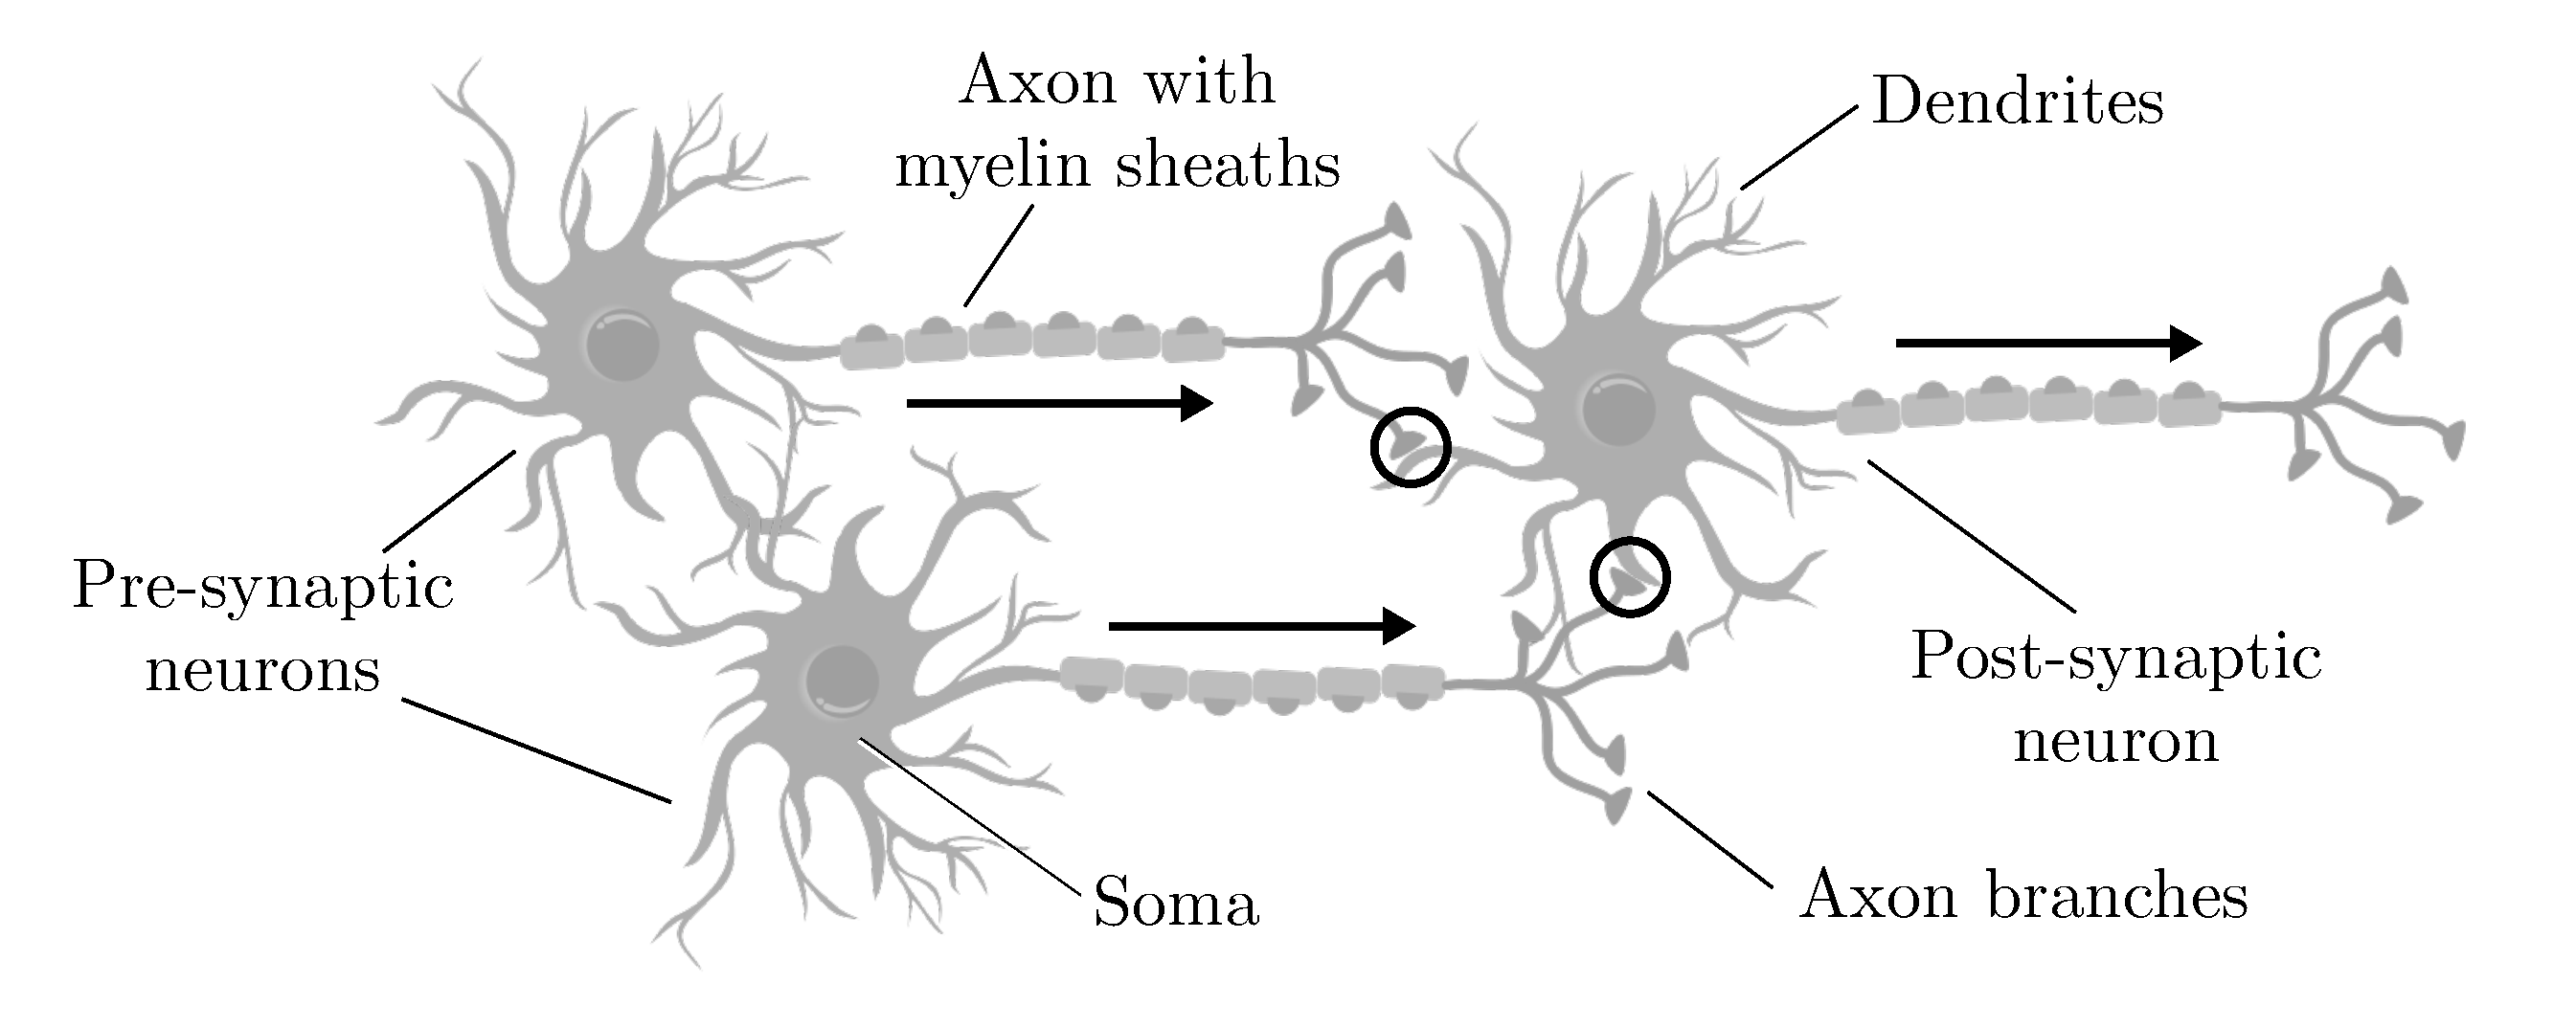
\includegraphics[width=0.8\textwidth]{neurons_plasticity/neurons}
	\caption[Structure of a typical neuron]{Three neurons showing the typical structure with soma, axon and dendrites. The synapses between presynaptic neurons and the postsynaptic neuron are highlighted with circles. The direction of the conduction is shown by arrows.\\ Adapted from: \emph{Set Of Neuron Vector.} (2017, December 16). Retrieved from https://www.vecteezy.com/vector-art/115973-set-of-neuron-vector}
	\label{fig:neurons}
\end{figure}

The dendrites and  the axon are called \emph{neurites}, which are projections from the cell body. The branches of the axon of one neuron are connected to another neurons dendrites. The connection points between the neurons are called synapses. In figure \ref{fig:neurons} a schematic representation of three neurons is shown where soma, dendrites and axon are indicated. The synapses are highlighted by circles.

\subsection{Action potential of a typical neuron}
\label{sec:act-pot}

According to \textcite{deetjen2005repetitorium}, a typical cell has a membrane potential of about $-70\,mV$ at its axon hillock, it is called the \emph{resting potential}. If the cell gets some electrical stimulation, which brings the membrane potential up to a \emph{threshold potential} of at least $-55\,mV$, the \emph{depolarisation} of the membrane potential starts, due to changes in the concentration of $Na^+$ and $K^+$ ions inside and outside of the cell. This is triggered by changes in the permeability of voltage-gated ion channels in the membrane of the neuron. The potential grows to about $40\,mV$, the \emph{action potential} or \emph{spike}. The action potential spreads over the neuron, mainly along the axon. If the axon is covered with myelin sheaths the propagation of the signal is called \emph{saltatory conduction}, which is faster than conduction without myelin sheaths.

The signals are transmitted nearly binary, where the threshold potential decides if the current activation is enough to transmit a signal or not. That principle is called \emph{all-or-none law}. The height of the threshold can vary, depending on two factors. First, directly after an activation potential was fired from the neuron, there is a short period, where the cell is not excitable at all (\emph{absolute refractory period}), which equals a threshold of infinity. After that, there is a period where the neuron is excitable again, but where the threshold is higher than normal (\emph{relative refractory period}). Both is due to ongoing recovery processes of ions in the cell. Second, the threshold is influenced by the extracellular concentration of ions, where also $Ca^{2+}$ plays an important role \parencite{deetjen2005repetitorium}.

\subsection{Structure and behavior of a typical synapse}
\label{sec:synapse}

The end of the axon or a branch of the axon of one cell (\emph{pre-synaptic cell}) is connected to the dentride of another cell (\emph{post-synaptic cell}). The cell membranes are called \emph{pre-synaptic membrane} and \emph{post-synaptic membrane} respectively. Both are shown in figure \ref{fig:synapse}.

Synapses can occur as a \emph{chemical synapse} or as an \emph{electrical synapse}. Chemical synapses transmit signals via chemical substances (\emph{neurotransmitter}), since the gap between the pre-synaptic and post-synaptic cell is $12\,nm$ to $20\,nm$ \parencite{savtchenko2007optimal} and cannot be bridged by electrical activation. The neurotransmitters need some time to reach the post-synaptic cell. Simulations show that it takes about $0.5\,ms$ until $50\%$ of the distributed transmitters receive the post-synaptic neuron, assuming a synaptic gap of $20\,nm$ \parencite{clements1996transmitter}. Electrical synapse are nearly directly connected with a gap of just $2\,nm - 3\,nm$ \parencite{peracchia1977gap}. They are connected by gap junction proteins, called \emph{connexins}, and can transmit electrical signals directly. In those synapses is nearly no delay in transmission compared to chemical synapses.

\begin{figure}[t]
	\centering
	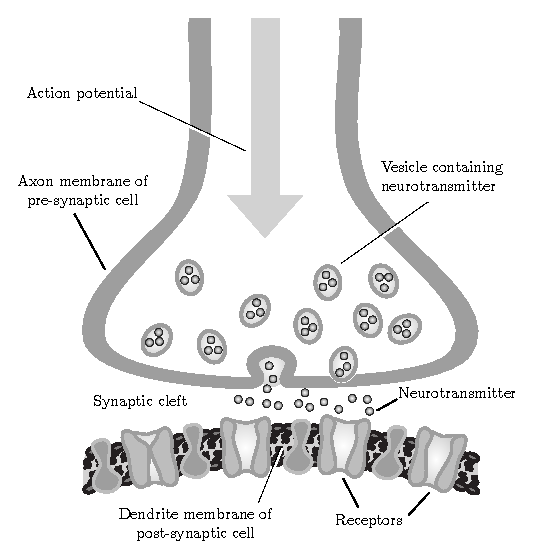
\includegraphics[width=0.6\textwidth]{neurons_plasticity/synapse}
	\caption[Structure of a typical synapse]{Structure of a typical chemical synapse. Because of an incoming potential, vesicles move to the synaptic cleft and release the containing neurotransmitter. The neurotransmitter will connect to the receptors in the membrane of the post-synaptic neuron. This causes a flow of ions in the post-synaptic membrane, changing its potential.\\ Adapted from: \textcite[p. 73]{schandry2007biologische}}
	\label{fig:synapse}
\end{figure}

In chemical synapses the pre-synaptic membrane contains the neurotransmitter, collected in \emph{vesicles}. If a potential arrives at the synapse, the vesicles move to the pre-synaptic membrane. The vesicles merge with the membrane and the neurotransmitters are released into the \emph{synaptic cleft}, the space between the pre-synaptic membrane and the post-synaptic membrane. At the post-synaptic membrane are receptors and ion channels, often they are joined to a \emph{receptor-channel-complex}. If they are combined to such a complex, the receptor is called \emph{ionotropic receptor}. The neurotransmitter binds to the ion channel and changes its structure which allows an exchange of ions. Since the neurotransmitter operates like a key which opens a lock, where the lock is the ion channel, this mechanism is called \emph{key-lock principle}. Since both parts (receptor and ion channel) are in one place, the reaction is fast \parencite[p. 40]{deetjen2005repetitorium}. In the other case, receptor and ion channels are separated and the receptor is called \emph{metabotropic receptor}. The neurotransmitter connects to a receptor, but this time the receptor releases a messenger substance called \emph{second messenger}. This second messenger finally opens an ion channel. The effect is slower, since it takes some time until the reaction inside the post-synaptic cell is ready and the ion channels are opened. A simplified scheme of a chemical synapse is shown in figure \ref{fig:synapse}.

\subsection{Inhibitory and excitatory neurons}
\label{sec:inhib-excit}

The signals, reaching the neuron via the synapses, can be \emph{inhibitory} or \emph{excitatory}. Inhibitory synapses reduce the potential and decrease the chance to reach the threshold potential that leads to an action potential. They mainly operate with GABA ($\gamma$-Aminobutyric acid), Glycine, Serotonin or Dopamin as neurotransmitter. Excitatory synapses rise the potential and therefore increase the chance to start an action potential. They mainly use Acetylcholine or Noradrenalin. Both types of synapses have different chemical mechanisms to change the potential. According to \emph{Dale's principle}, a neuron has either only inhibitory or excitatory axonal synapses \parencite{dale1935pharmacology, eccles1976electrical}. There are exceptions from this rule, but in most cases the principle holds \parencite{sossin1990dale}. If a neuron has inhibitory outgoing synapses, it is called an \emph{inhibitory neuron}. In case of excitatory synapses it is called \emph{excitatory neuron}.

The incoming signals from all connected synapses --- which can be several thousands \parencite[p. 89]{schandry2007biologische} --- sum up to an overall potential at the soma of the post-synaptic neuron. The summation can be spatial or temporal. \emph{Spatial summation} means that the potential is rising if many different synapses are active at the same time. \emph{Temporal summation} describes a process where at a synapse many signals are coming in a row and sum up to a higher overall potential. The time gap between the signals can be very different, depending on the type of synapse. In some synapse it is necessary, that the signals must be closer than $20\,ms$ to each other to have a summing effect, in some synapses a gap of $1\,s$ can still influence the potential \parencite[p. 92]{schandry2007biologische}.

In many artificial networks the neuron $i$ is modeled with a specific activation $a_i$ at a time, which is linearly dependent from incoming signals. In that case spatial summation can be modeled with

\begin{equation}
\label{eq:activation}
a_i = \sum_{j=1}^{n_i} w_{ij} z_{j} - t_i,
\end{equation}

where $n_i$ is the number of potential input signals (number of synapses), $z_{j}$ the activation of the single sources and $w_{ij}$ the weights from the pre-synaptic neuron to the post-synaptic neuron. $t_i$ is the threshold of the post-synaptic neuron.

The transmission of a signal from one neuron to another is modeled with an \emph{activation function} $\sigma(a_i)$ that modulates the intensity and can decide if the neuron is sending a signal or not. To model the binary output of a biological network an indicator function can be used, like the \emph{Heaviside step function}

\nomenclature{$\sigma(a_i)$}{Activation function}

\begin{equation}
\label{eq:heavi}
\sigma(a_i) = \Theta(a_i) = \begin{cases}
\;0, & a_i < 0\\
\;1, & a_i \ge 0
\end{cases}.
\end{equation}

If the activation $\sum_{j=1}^{n_i} w_{ij} z_{j}$, coming from the pre-synaptic neurons, is higher than the threshold $t_i$, the Heaviside function is equal to one and an action potential of the post-synaptic neuron is simulated.

In many cases it is necessary to calculate derivations of the activation function (e.g. for the backpropagation algorithm, which is widely used in machine learning). In that case smooth approximations like the sigmoid function can be used. Statistically the activation function $\sigma$ is the inverse of the link function in a \acfi{glm} and therefore the part that brings non-linearity to the model, since $a_i$ is a linear function. In case of the sigmoid function, the activation function at every neuron is equal to a logistic regression. Further details regarding the mathematical model are given in section \ref{sec:ann}.

\subsection{Classifications of neurons}

In general, neurons can be classified by their function \parencite[p. 39]{schandry2007biologische}.

\begin{itemize}
\item \emph{Sensory neurons}: Receives information from a sensory cell
\item \emph{Motor neurons}: The axon is connected to a muscle
\item \emph{Interneurons}: The most common type, which receives from and sends information to other neurons
\end{itemize}

In artificial neural networks the \emph{input} can be seen as sensory neurons in living beings, where the whole network structure is equivalent to the interneurons. The \emph{readout} of a network is analog to the current state of the interneurons. The \emph{output} is similar to the motor neurons which could, for instance in robotics, control some electric motors.

Neurons can also be classified morphologically.

\begin{enumerate}
\item \emph{Unipolar neuron}: Has just one neurite, mostly one axon
\item \emph{Bipolar neuron}: Has two neurites, one axon and one dendrite
\item \emph{Multipolar neuron}: Has many neurites, one axon and many dendrites
\item \emph{Anaxonic neuron}: Axon and dendrites cannot be differentiated
\end{enumerate}

\begin{wrapfigure}{r}{0.45\textwidth}
	\centering
	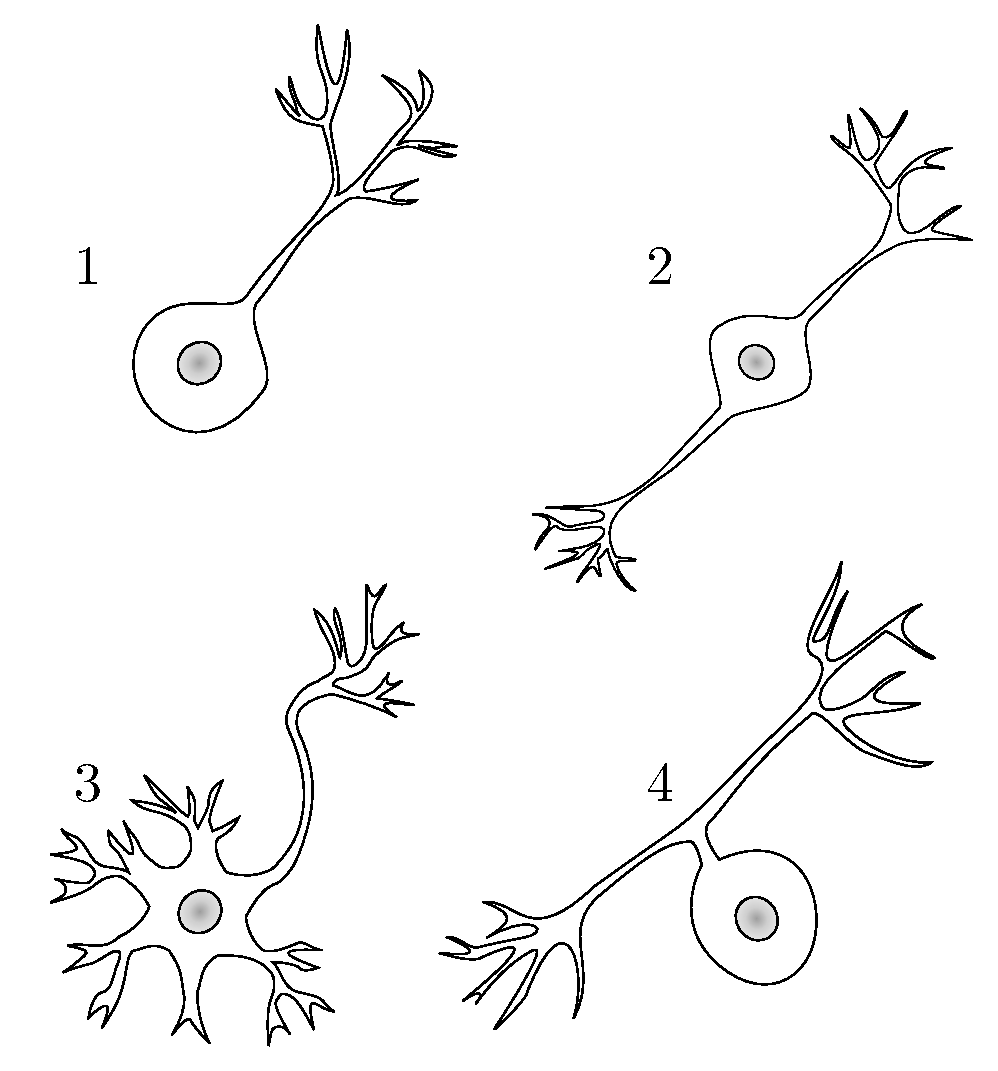
\includegraphics[width=0.45\textwidth]{neurons_plasticity/neuron_types}
	\caption[Morphological classification of neurons]{Morphological classification of neurons: (1) Unipolar neuron, (2) Bipolar neuron, (3) Multipolar neuron and (4) Anaxonic neuron.\\ Adapted from: \emph{Neuron.} (2017, December 16). Retrieved from https://en.wikipedia.org/wiki/Neuron}
    \vspace{10pt}
    \label{sec:neuron-types}
\end{wrapfigure}

All four types are are shown in figure \ref{sec:neuron-types}. There are many specialized cells like for example purkinje cells, which are large multiplolar interneurons in cerebellum, or pyramidal cells, which are multipolar interneurons in many areas of the brain. Pyramidal cells, for example, are the main source for measurements using electroencephalography \parencite{kirschstein2009source}.

In many artificial networks, like the one which is used in this thesis, the input is designed with a neuron which has just an axon with some projections, the output has just dendrites. Inbetween are multipolar or rarely bipolar neurons, which form the characterizing part of the artificial neural network. As well as in the brains of living beings, the most common neuron in artificial neural networks is modeled with the multipolar neuron.


\section{Plasticity}
\label{sec:plasticity}

Plasticity or more specific \emph{neuroplasticity}, when it comes to brains, is the ability of the brain to change its neuronal structure depending on experience. It can be separated in \emph{functional plasticity} and \emph{structural plasticity}.

\begin{itemize}
\item Functional plasticity: Changes in synaptic transmission characteristics due to changes in amount of neurotransmitter or receptors
\item Structural plasticity: Changes in structure of the neuron, like growing or shrinking of axons, dendrites, synapses or even whole neurons
\end{itemize}

Furthermore, \emph{synaptic plasticity} describes all processes related to synapses, like changes in transmission characteristics and growing or shrinking of synapses. Regarding synaptic plasticity one can distinguish between \emph{pre-synaptic plasticity} and \emph{post-synaptic plasticity}. Pre-synaptic plasticity means, that the amount of released neurotransmitters or the time for readmission of neurotransmitters changes. Post-synaptic plasticity changes the sensibility for a given amount of neurotransmitters. For example the amount of receptors (ion channels) can be adapted. Furthermore, plasticity can vary in duration. \emph{Short-term plasticity} changes the transmission characteristic of the synapses in a scale of milliseconds to minutes, while \emph{long-term plasticity} has an effect for hours, or even years. Both can be separated in so called depression --- \acf{std} and \acf{ltd} --- which means a decrease in connectivity, and potentiation --- \acf{stp} and \acf{ltp} --- which means an increase in connectivity between the synapses.

Second messengers (see above in section \ref{sec:synapse}) play an important role in synaptic plasticity \parencite{skrebitskiui1999synaptic}. Metabotropic receptors can not only start mechanisms to open ion channels, they can also start processes to change the behavior of receptors, channels or neurotransmitters.

In artificial neural networks the synaptic transmission characteristic can be modeled as a weight $w_{ij}$ between neuron $i$ and neuron $j$, as already used in equation \eqref{eq:activation}. If there is no connection between two neurons, it holds that $w_{ij} = 0$. Functional plasticity corresponds to a change in $w_{ij} \in (0,1]$, indicated as $\Delta w_{ij}$, whereby structural plasticity sets the weight to zero or non-zero.

\subsection{Hebb's rule}

A rule that simplifies a functional plasticity mechanism is the \emph{Hebb rule}. Biologically, synapses strengthen their connection if the firing of neuron $j$ and the firing of neuron $i$ is close together. In that case the weight $w_{ij}$ will increase.

\begin{figure}[!b]
	\centering
	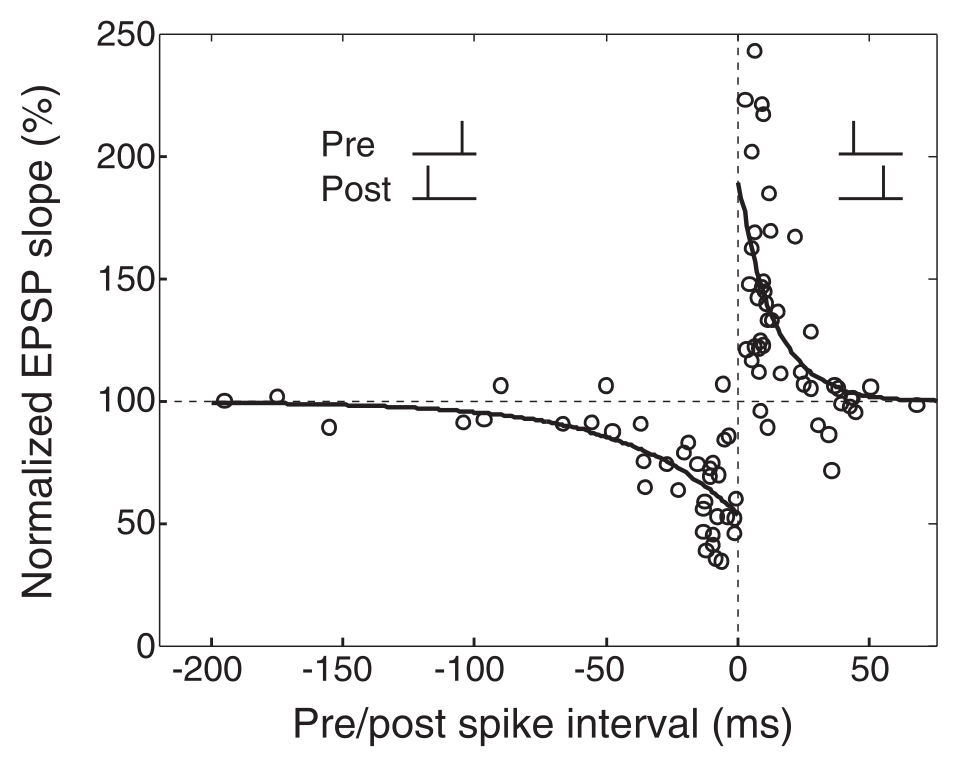
\includegraphics[width=0.6\textwidth]{neurons_plasticity/stdp.png}
	\caption[Spike-timing-dependent plasticity]{Spike-timing-dependent plasticity \parencite[figure 1]{dan2006spike}. The closer the post-synaptic neuron spikes before the pre-synaptic neuron spikes, the higher will be the \emph{decrease} in weight and vice versa.}
	\label{fig:stdp}
\end{figure}

For artificial neural networks holds therefore

\begin{equation}
\Delta w_{ij} = \eta \cdot z_j \cdot a_i,
\end{equation}

where $\eta$ is a learning rate. A high learning rate results in fast but inaccurate convergence, while a low learning rate results in slow but accurate convergence.

\subsection{Spike-timing-dependent plasticity}

The \acfi{stdp} is a causal type of Hebb's rule, depending on temporal correlations between the spikes of pre-synaptic and post-synaptic neurons \parencite{sjostrom2010spike}. Spikes arriving repeatedly at the pre-synapses, some time before or after an action potential at the post-synaptic neuron, lead to long-term plasticity. In case that spikes arrive shortly before an action potential of the post-synaptic neuron, it leads to \acl{ltp}. In case that spikes arrive shortly after an action potential of the post-synaptic neuron, it leads to \acl{ltd}. The time scale where plasticity occurs, varies between different types of synapses. In most cases it is of the order of milliseconds \parencite{dan2006spike}. An illustration of the \acs{stdp} is shown in figure \ref{fig:stdp}.

\begin{wrapfigure}{R}{0.45\textwidth}
	\centering
	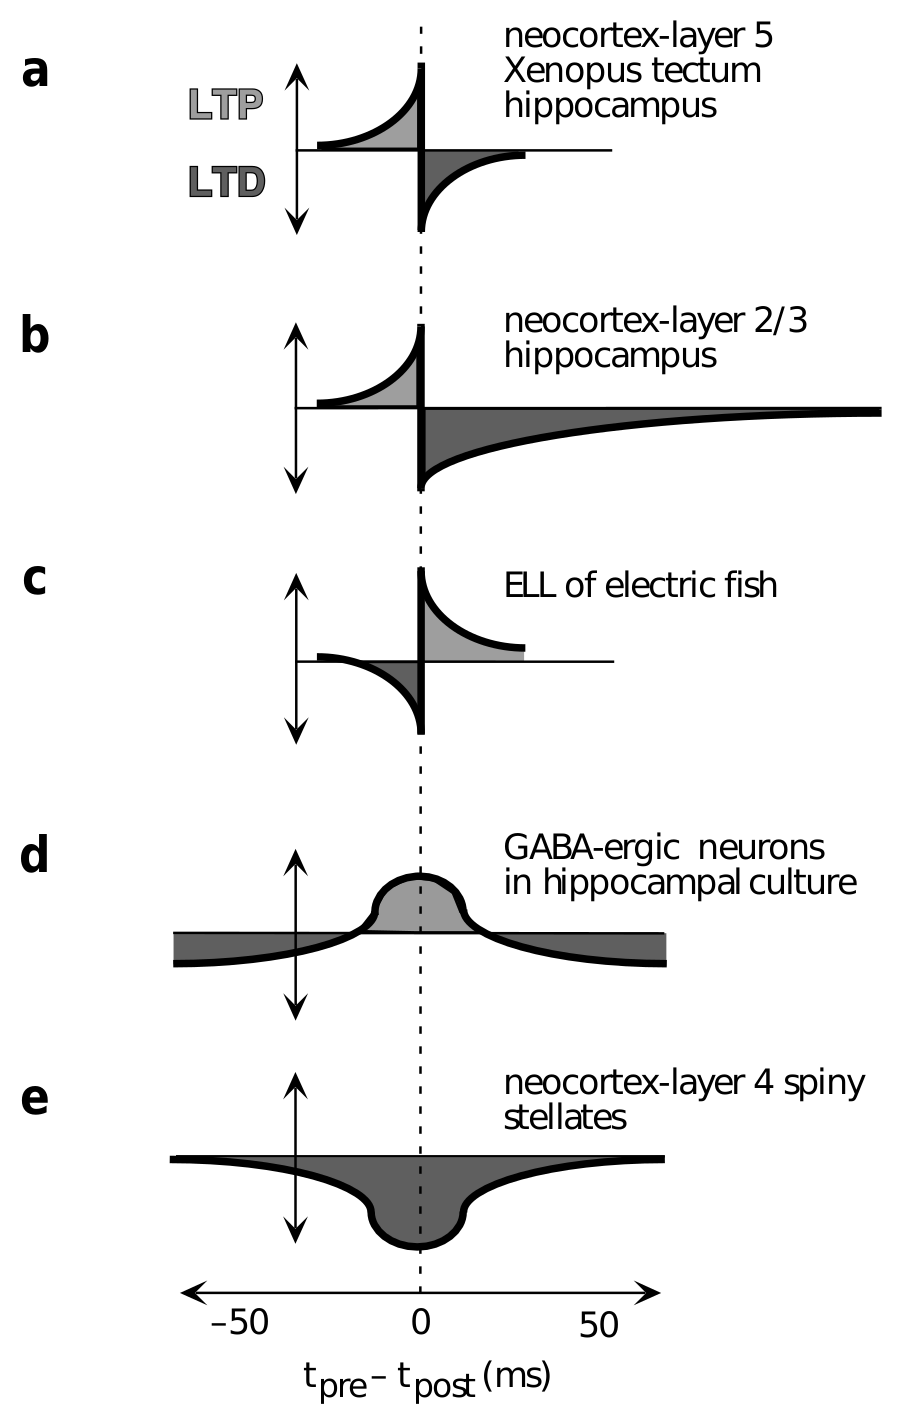
\includegraphics[width=0.45\textwidth]{neurons_plasticity/learning-window.png}
	\caption[Learning windows]{\ac{stdp} learning windows \parencite[figure 2]{abbott2000synaptic}.}
    \label{fig:learning-windows}
    \vspace{-10pt}
\end{wrapfigure}

A mathematically formulation of the \ac{stdp} was done by \textcite{sjostrom2010spike} and more specific by \textcite{kempter1999hebbian}. Consider a post-synaptic neuron with activity $x_i(t)$ and a pre-synaptic neuron with activity $x_j(t)$. Assume many spikes at the post-synaptic neuron, counted by $l \in \{ 1,...,n_l \}$, where $n_l$ is the total number of spikes. $t_i^l$ indicates the time for every spike at neuron $i$ with $x_i(t_i^l) = 1$. Furthermore, the number of spikes of the pre-synaptic neurons is counted by $k \in \{ 1,...,n_k \}$, where $n_k$ is the total number of spikes. $t_j^k$ indicates the points in time at which the pre-synaptic neuron is firing with $x_j(t_j^k) = 1$.

The \emph{learning window} is a function $f(\Delta t)$, where $\Delta t = t_j^k - t_i^l$. It can be defined in various ways, some are shown in figure \ref{fig:learning-windows}. Using the learning window, the change of the weight can be defined as

\begin{equation}
\label{eq:stdp-orig}
\Delta w_{ij} = \sum_{k=1}^{n_k} \sum_{l=1}^{n_l} f(\Delta t) = \sum_{k=1}^{n_k} \sum_{l=1}^{n_l} f(t_j^k - t_i^l).
\end{equation}

$f(\Delta t)$ is often chosen as an exponential function \parencite{sjostrom2010spike}. It could be shown, that an exponential learning window is able to model experimental findings \parencite{zhang1998critical}. It can be defined as

\begin{equation}
f(\Delta t) = \begin{cases}
\;A_+ \exp(-\Delta t / \tau_+), & x > 0\\
\;-A_- \exp(\Delta t / \tau_-), & x < 0
\end{cases},
\end{equation}

where $A_+$ and $A_-$ are parameters to choose. $\tau_+$ and $\tau_-$ are time constants and often chosen as $\tau_+ = \tau_- = 10\,ms$.

If, for the exponential learning window, $t_j^k$ and $t_i^l$ are close to each other most of the time, which means that pre- and post-synaptic neurons spiking in succession, there will be a change in the weight between those neurons, depending on the sign. The more often those neurons fire close to each other, the higher will be the sum and the change of the weight. The principle of the exponential learning window is shown in figure \ref{fig:learning-windows}a.

For simulations of neural networks which are focused on more high level network based research, \ac{stdp} is often modeled more simple. One simplified version, where the weight only depends on the spiking between two discrete time steps, will be introduced in section \ref{sec:sorn}.

\subsection{Homeostatic plasticity}

A network just processing Hebb's rule would soon end in a destabilized state. If \acs{ltp} becomes dominant, the synapses in the network will increase unbounded. If \acs{ltd} becomes dominant, the synapses will decrease to zero at some point. Hence, the synaptic activity in the network is diverging and therefore needs constraints \parencite{miller1994role, abbott2000synaptic}. In figure \ref{fig:homeo} the stability problem is shown for a simplified example. A small feed forward network with $5$ layers is only able to propagate an input signal if the gain is close to $1$. If it is higher than $1$, the activity `explodes' and the sinusoidal input signal cannot be represented in the last layer. Otherwise, if the gain is lower than $1$, the signal `dies out' and is not able to reach the last layer. The same holds for recurrent networks, where the problem of propagation happens in time, compared to propagation in space regarding the layers in a feed forward structure \parencite{turrigiano2004homeostatic}. In machine learning this problem is known as the \emph{exploding and vanishing gradient problem} \parencite{pascanu2013difficulty}.

\acs{stdp} can allow some more stability than Hebb's rule alone \parencite{abbott2000synaptic}, depending on the learning window, which leads to more precise \acs{ltp} and \acs{ltd}. The ability, how much \acs{stdp} is able to stabilize the network, depends on the parameters of $f(\Delta t)$.

However, biologically, one can observe a whole set of different constraints which appear in natural neural networks in order to maintain a specific target firing rate. They are reviewed for example by \textcite{turrigiano2004homeostatic}, \textcite{turrigiano2008self}, \textcite{pozo2010unraveling} and \textcite{turrigiano2012homeostatic} and summarized at Scholarpedia by \textcite{williams2013homeostatic}. The main goal of those processes is to keep a specific activity in the network. It acts as a set point or baseline for the overall activity. If some areas in the network are going up in activity for some time, the networks reacts with a re-normalization of the whole activity, where the relative connections between the neurons stay the same. It is important to note that those mechanisms operate in a decentralized way, where every neuron adjusts for itself. There cannot be any centralized power, controlling the overall activity. This kind of plasticity is called \emph{homeostatic plasticity}. There are several different complex mechanisms of homeostatic plasticity and some of them are still not fully understood. However, those mechanisms can be classified by:

\begin{figure}[t]
	\centering
	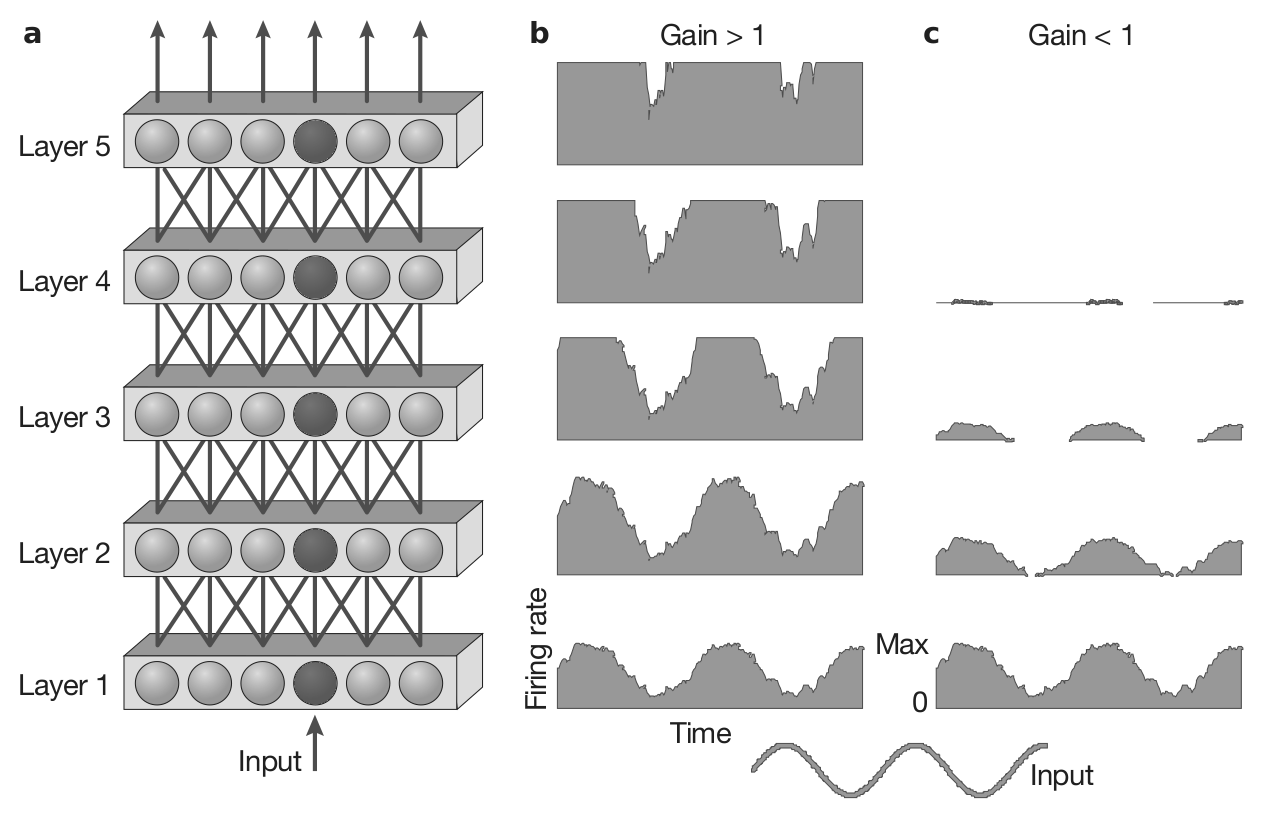
\includegraphics[width=0.6\textwidth]{neurons_plasticity/homeostatic-problem.png}
	\caption[Instability of networks]{Instability of networks for a simplified case \parencite[figure 1]{turrigiano2004homeostatic}. \textbf{a)} A small feed forward network with $5$ layers, the activity of the dark neuron is shown in b and c. \textbf{b)} If the gain is higher than $1$, the activity `explodes' and the sinusoidal input signal cannot be represented in the last layer. \textbf{c)} If the gain is lower than $1$, the signal `dies out' and is not able to reach the last layer.}
	\label{fig:homeo}
\end{figure}

\begin{itemize}
\item Type: Intrinsic (affecting the neuron) or synaptic (pre-synaptic and post-synaptic)
\item Spatial: More global (all synapses connected to a neuron) and more local or quasi-local (single synapse or small groups of synapses connected to a neuron)
\item Temporal: Fast (seconds to hours) and slow (hours to days)
\end{itemize}

\subsection{Synaptic normalization}
\label{sec:synaptic-scaling}

One important class of synaptic homeostatic plasticity is \emph{synaptic scaling}, where incoming synaptic connections to a neuron are normalized to a target weight. While adjusting the weights, their relative strengths are maintained. \textcite{turrigiano2008self} summarizes that neurons use calcium-dependent sensors to detect changes in their own firing rates. Depending on those changes the number of receptors at the synapses will be regulated. Note that the more local the mechanisms are and the fewer synapses are involved, the more the synaptic scaling mechanism will interact with \ac{ltd} and \ac{ltp} mechanisms, like \ac{stdp}.

While the normalizing process is highly complex in natural networks, in artificial systems it is relatively simple to perform. For example, in a simplified more global rule, every weight connected to a neuron $i$ is just normalized with all incoming weights from neurons $j$, using

\begin{equation}
\label{eq:sn}
w_{ij}(t) \leftarrow \frac{w_{ij}(t)}{\sum_{j=1}^N w_{ij}(t)},
\end{equation}

\nomenclature{$w_{ij}$}{Weight between neuron $i$ and neuron $j$}

where $w_{ij}(t)$ is the weight between neuron $i$ and $j$ at time $t$. Due to the mathematical process of normalization, it is also called \emph{synaptic normalization}.

\subsection{Intrinsic plasticity}
\label{sec:ip}

\ACFI{ip} is a process, which is local and intrinsic, since it only affects the conduction inside of a single neuron. In \acs{ip} no synapse and therefore, when modeling artificial networks, no weight is affected. There are several different types of \acl{ip} and many of them are not fully understood \parencite{cudmore2008intrinsic}. In principal, the neuron regulates biophysical properties of ion channels in the membrane. \textcite{awatramani2005modulation} showed that a small depolarization of about $10\,ms$ (resulting in a potential between $-60\,mV$ and $-65\,mV$), induced by a change of the extracellular concentration of calcium ions, enhances the probability of transmitter release up to $2$-fold.

\begin{wrapfigure}{R}{0.45\textwidth}
	\centering
	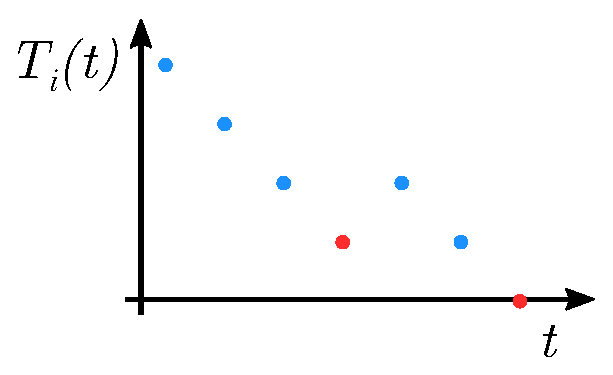
\includegraphics[width=0.45\textwidth]{neurons_plasticity/ip}
    \caption[Intrinsic plasticity and spontaneous activity]{Simple implementation of intrinsic plasticity. If the neuron is not spiking (blue dot), the threshold is decreased in the next step of time. If the neuron is spiking (red dot), the threshold is increased in the next step of time. If the threshold moves below zero, the neuron fires spontaneously.}
    \vspace{10pt}
    \label{fig:intrinsic-plasticity}
\end{wrapfigure}

A simple implementation in artificial neural networks affects the threshold for conducting the action potential inside of the neuron. If the neuron was active, the threshold will increase for the next step. If the neuron was not active, the threshold will decrease, to make the neuron more sensible. Note that if the threshold of a neuron becomes negative, the neuron fires spontaneously. The effect is shown in figure \ref{fig:intrinsic-plasticity}. The rule can be formalized with

\begin{equation}
\label{eq:ip}
T_i(t+1) = T_i(t) + \eta_\IP \left( x_i(t) - H_\IP \right),
\end{equation}

\nomenclature{$\eta_\IP$}{Learning rate for intrinsic plasticity}
\nomenclature{$T_i(t)$}{Threshold of neuron $i$ at time $t$}

where $\eta_\IP$ is the learning rate and $x_i(t) \in \{0,1\}$ the activity of neuron $i$ at time $t$. $H_\IP$ is the \emph{target rate}. All neurons will in average be active with a rate of $H_\IP$. The choice of $H_\IP$ is not trivial, since not all choices of the target rate will necessarily lead to a network with good performance \parencite{lazar2009sorn}.


\section{Self-organizing recurrent neural network (SORN)}
\label{sec:nn}

\subsection{Artificial neural networks}
\label{sec:ann}

Two different scientific approaches motivate an \acfi{ann}. Originally those networks were invented to simulate processes in the brain to get a better understanding of how the brain stores and processes information and how recognition and behavior is influenced by neural activity. Especially \textcite{rosenblatt1958perceptron} formulated a first idea to simulate a simple neural system, the so called \emph{perceptron}. On the other side, the idea came up to construct classification and prediction algorithms using \acs{ann}. Even though the approach was promising, for a long time artificial networks were not useful, because networks are computational costly and need big datasets to perform well. But when \textcite{hinton2006fast} published a fast way to train \acs{ann} and computers became more powerful at the same time, \acs{ann} became a widely used approach in machine learning. In machine learning \emph{supervised} \acs{ann}, where the algorithms learns with a given `truth', are still inspired by biology, but in most cases very different from real neural networks. On the other hand, computational neuroscience uses mostly \emph{unsupervised} networks, since there is no evidence that humans learn from an absolute truth. Those networks mostly try to be as close as possible to real neural processes or try to understand specific properties of biological networks. Nevertheless, in computational neuroscience the used networks highly depend on the level of research. For research on cell level, many details of neural conduction and synapses behaviors are modeled. Otherwise, if models on higher levels with hundreds or thousands of neurons are build, e.g. modeling memory and learning, many biological details on cell level are omitted in order to reduce complexity.

Independent of the approach, the basic principle for modeling neurons is the perceptron. Statistically the perceptron can be understood as a \ac{glm}, classifying the incoming signals either directly as $0$ or $1$ or giving a probability for those classes.

Beginning with a regression model, some inputs $\bm x \in \R^d$ are chosen to describe some output $y \in \R$, using a \emph{regression function} $f(\bm x)$. The regression is of the form

\begin{equation}
y = f(\bm x) + \epsilon.
\label{eq:gen-reg}
\end{equation}

Instead of the direct data $\bm x$ it is also possible to use a transformation $\phi(\bm x)$, which is called a \emph{feature}. For modeling a neural network, data $\bm x$ is used directly. $\epsilon \in \R$ is a stochastic error term, a random variable, and can be distributed in several ways. In most applications it is assumed to be normally i.i.d. distributed with $\epsilon \sim N(0,1)$. The regression function $f(\bm x)$ can be arbitrary. In a linear case it has the form

\begin{equation}
f(\bm x) = \bm x^T \bm \beta,
\end{equation}

where $\bm \beta \in \R^d$ are the parameters of dimension $d$. While the estimator of a linear model is relatively easy to obtain, an estimator for a non-linear $f(\bm x)$ is not easy to find. In order to have the opportunity to use non-linear models, in \ac{glm}s a so called link function $g^{-1}(f(\bm x)) = g^{-1}(\bm x^T \bm \beta)$ is introduced. It brings non-linearity to a linear model. If the expected value of $y$, modeled with the link function, is taken, it results in

\begin{equation}
\mu = \E[y] = \E[g^{-1}(\bm x^T \bm \beta) + \epsilon] = g^{-1}(\bm x^T \bm \beta),
\end{equation}

since $g^{-1}(\bm x^T \bm \beta)$ is deterministic and $\E[\epsilon] = 0$. At that point, the derived statistical model can be mapped to an \acs{ann} use case. $\bm x$ can be identified with the input signals from all pre-synaptic neurons $\bm z$ from equation \eqref{eq:activation}, where the first input is a dummy and is set to one. Furthermore, it can be seen that $\bm\beta$ is equal to the weights $\bm w_i$, where the first weight is $-b_i$. It means that $\sum_{j=1}^{n_i} w_{ij} z_j - b_i = \bm x_j^T \bm\beta_j$. Finally, the inverse of the link function $g^{-1} = \sigma$ is the \emph{activation function}, introduced in section \ref{sec:inhib-excit}, and $o = \mu$ denotes the output at the post-synaptic neuron. The output is given by

\begin{equation}
\label{eq:ann-model}
\mu = g^{-1}(\bm x^T \bm \beta) = g^{-1}\left(\sum_{j=1}^{n_i} w_{ij} z_j - b_i\right) \overset{\eqref{eq:activation}}{=} \sigma(a_i) = o.
\end{equation}

As already discussed in section \ref{sec:inhib-excit}, the choice of the activation function depends on the requirement. In machine learning, classically, a continuous function like a sigmoid or, more recent, piecewise rectified linear units (ReLUs) are used, since derivations are often necessary. In that case, there is always some activation, which rises strongly, if the input neurons increase in activity. Statistically, the perceptron with a sigmoid function is a logistic regression. 
 
In case of an indicator function, an all-or-none law is realized, which is a closer approximation to real neurons. It results in zero activity, if the input neurons sum to a value below the threshold and an activity of one, if the sum of the activity hits the threshold. Such an indicator function was introduced in equation \eqref{eq:heavi}.

So far, the perceptron model is able to simulate some pre-synaptic neurons and one post-synaptic neuron, which depends on the activity of the pre-synaptic neurons and the activation function. If multiple perceptrons are modeled, the output of one neuron can be an input for another neuron and so forth. Mathematically, a neural network with multiple neurons is a recursive \acl{glm}. It can be modeled in one direction with a \emph{feed forward} structure or in arbitrary directions with a \emph{recurrent} structure.

\subsection{Classification of ANN}

Over time, a large number of network types were developed. Besides many different architectural types, two important types will be mentioned here:

\begin{itemize}
\item \emph{Feed-forward neural networks} are basically multilayer perceptrons, where synapses are just built in one direction. The flow of information is going from input neurons to output neurons with hidden layers inbetween.
\item \ACFI{rnn} have neurons which have synapses not only reaching into the next layer, but also to a neuron in next time step of processing. Therefore, time-coded information can be included.
\end{itemize}

Another possible classification refers to the number of connections. A \emph{fully connected} network has all connections established, and therefore weights of non-zero between all neurons. A \emph{sparsely connected} network has just some few connections, whereas most connections are fixed to zero. In some networks, like Echo State Networks (see below), the connectivity is in an order of about $1\%$.

\subsection{Reservoir Networks}
\label{sec:res-net}

A specific case of \acs{rnn} is \emph{Reservoir Computing} \parencite{lukovsevivcius2009reservoir}. Those networks can be called reservoir networks. Input signals are fed into a sparsely and randomly connected network, called \emph{reservoir}. The reservoir behaves like a complex nonlinear dynamic filter that transforms the incoming signals using a high-dimensional temporal mapping \parencite{schrauwen2007overview}. Schrauwen et al. described similarities between reservoir computing and kernel methods. Kernel methods are often used in machine learning to transform the input into a multi-dimensional or even infinite-dimensional feature space, where linear separation or linear fitting performs better than in the original input space. Similar to kernels, also a reservoir can be seen as a transformation of the input into higher dimensions, where the readout is kind of a feature space. If the reservoir contains $N$ neurons, the input is projected into a $N$-dimensional space. A state of the reservoir is mathematically just a point in this high dimensional space. Temporal signals entering the reservoir can be described as a trajectory in that space. \textcite{lazarphd2009self} hypothesized in her dissertation that, theoretically, the brain computes with trajectories in a similar way, which would justify the use of reservoir networks in neural computation approaches.

Two major types of Reservoir Networks are \ac{esn} \parencite{jaeger2004harnessing} and \ac{lsm} \parencite{maass2002real}. Both networks were independently developed \parencite{goodfellow2007deep} and are quite similar. \ac{lsm} uses neurons with binary outputs. They are designed to explain processes in the brain, whereas \ac{esn} uses continuous hidden units and focuses on machine learning tasks. Under the condition of the \emph{separation property} (different inputs result in separable outputs) and the \emph{fading memory property} (information about recent input can be maintained) the \ac{lsm} fulfills the Stone-Weierstrass theorem, namely that the \ac{lsm} can approximate any continuous function \parencite{maass2004computational}. Therefore \ac{lsm} is an interesting starting point for reservoir based neural simulation.

\subsection{Self-organizing recurrent neural network (SORN)}
\label{sec:sorn}

\ac{lsm} are developed for supervised learning and parameters are trained in a way to minimize the error. To simulate brain dynamics it is necessary to find a more unsupervised way of learning. Furthermore, those networks have normally a static reservoir, which means that the weights are randomly initialized and fixed in further processing. To tackle both problems, plasticity rules are a promising approach. They could be used as described in section \ref{sec:plasticity}. There were already some additions to \acl{lsm}, like adding hebbian learning \parencite{norton2006preparing}, but a first sophisticated reservoir network with plasticity was proposed by \textcite{lazar2009sorn}, called a \acfi{sorn}. It uses three plasticity rules in a reservoir network with binary threshold neurons, namely:

\begin{itemize}
\item \ACF{stdp}
\item \ACF{sn}
\item \ACF{ip}
\end{itemize}

\paragraph{Plasticity rules}

\begin{wrapfigure}{R}{0.45\textwidth}
	\centering
	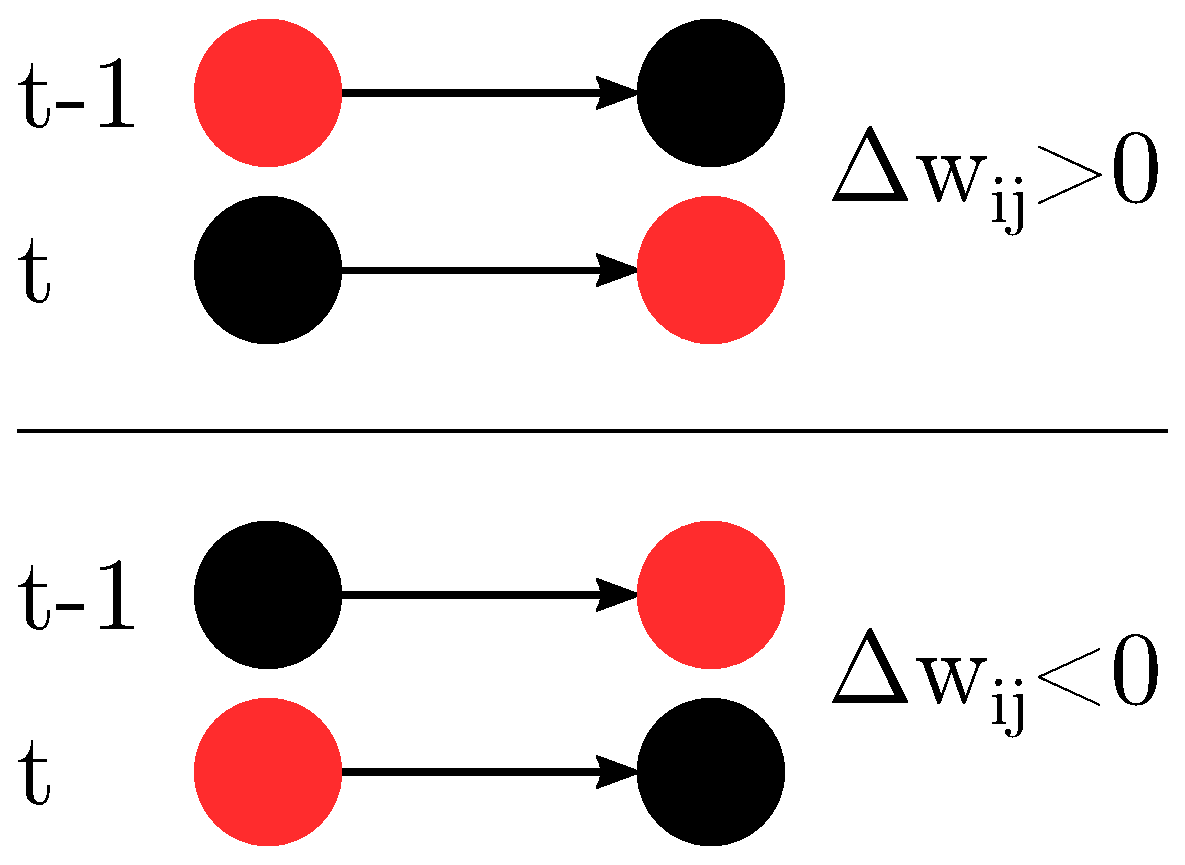
\includegraphics[width=0.45\textwidth]{sorn_markov/stdp}
    \caption[Spike-timing-dependent plasticity rule used in \acs{sorn}.]{Spike-timing-dependent plasticity rule used in \acs{sorn}. The black circle corresponds to a silent neuron, the red circle represents a spiking neuron. The arrow indicates the direction of the weight. If the pre-synaptic neuron is firing, before the post-synaptic neuron fires, the weight between them is increased. Otherwise, the weight is decreased.}
    \label{fig:stdp-simple}
\end{wrapfigure}

The \acl{sn} and \acl{ip} are realized according to equation \eqref{eq:sn} and equation \eqref{eq:ip} respectively. Regarding the \acs{ip}, recall that it is the source for spontaneous activity. \acs{sorn} is build such that noise is optional and in most applications the network is using spontaneous activity from \acs{ip} only. In consequence the system can be described as deterministic chaos, if the initial weights are given. Only if noise is included, it would truly behave stochastically. The only remaining stochastic part is the random initialization of the weights.

The \acl{stdp} can be derived from equation \eqref{eq:stdp-orig}. In \acs{sorn} only the last step in time and thus only one spike is considered. If the pre-synaptic neuron fires directly before the post-synaptic neuron, the weight is increased. Otherwise, the weight is decreased, as shown in figure \ref{fig:stdp-simple}. Hence, there is no summing necessary and the rule is simplified to

\begin{equation}
\Delta w_{ij}(t) = f(\Delta t) = f(t_j - t_i),
\end{equation}

where $t_j$ is the time when the pre-synaptic neuron $j$ spikes and $t_i$ when the post-synaptic neuron $i$ spikes. The learning window is defined as

\begin{equation}
f(\Delta t)
= \eta_\STDP \cdot \begin{cases} x_j(t_i - 1) x_i(t_i) & t_j \le t_i\\ -x_j(t_j) x_i(t_j - 1) & t_j > t_i \end{cases},
\end{equation}

\nomenclature{$\eta_\STDP$}{Learning rate for \acl{stdp}}

where the learning rate $\eta_\STDP$ was introduced. Note that $f(\Delta t)$ is zero, if both neurons are not active in a row. If $t$ denotes the absolute time of the network, the weight change can be simplified to

\begin{equation}
\label{eq:stdp}
\Delta w_{ij}(t) = \eta_\STDP \cdot \left( x_j(t-1) x_i(t) - x_j(t) x_i(t-1) \right),
\end{equation}

since $x_i(t), x_j(t) \in \{0,1\}$. Equation \eqref{eq:stdp} corresponds to \textcite[equation 5]{lazar2009sorn}.

What kind of plasticity rule is used, depends on the phase of training and testing. All the rules, which are included in a phase are applied after every discrete calculation step.

\paragraph{Network setup}

\nomenclature{$N^E$}{Number of excitatory neurons}
\nomenclature{$N^I$}{Number of inhibitory neurons}

\nomenclature{$W$}{Weight matrix}

\begin{figure}[t]
	\centering
	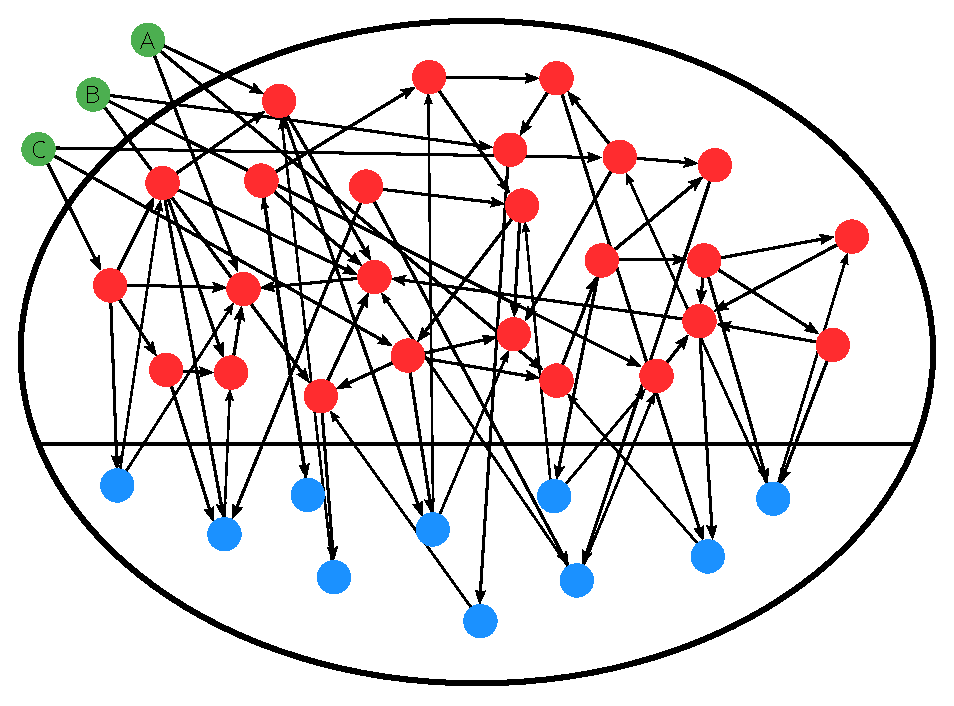
\includegraphics[width=0.6\textwidth]{sorn_markov/sorn}
	\caption[Sketch of the \acl{sorn}]{Sketch of the \acl{sorn}. Red circles are excitatory neurons, blue circles represent inhibitory neurons. Connections between excitatory neurons are sparse, inhibitory and excitatory neurons are fully connected in both directions. Input neurons are represented by green circles. They are connected to excitatory neurons.}
	\label{fig:sorn}
\end{figure}

$N^U$ is the number of input neurons and $N^E$ the number of excitatory neurons. Excitatory and inhibitory neurons were separated. The number of inhibitory neurons is set as a fraction of excitatory neurons, for example $N^I = 0.2 \cdot N^E$. All neurons have a weight of $w_{ij} \in [0,1]$. Weights are established between excitatory and excitatory neurons, modeled in a matrix $W^{EE}$, between inhibitory and excitatory neurons $W^{EI}$, excitatory and inhibitory neurons $W^{IE}$ and input neurons and excitatory neurons $W^{EU}$. The matrices $W^{EI}$ and $W^{IE}$ are fully connected, $W^{EE}$ is sparsely connected.

There are no connections between inhibitory and inhibitory neurons in the model. While those connections exist in real biological networks, they occur sparsely and their function is highly specialized \parencite{chamberland2012inhibitory}. Important are connections between excitatory and inhibitory neurons and vice versa. Those connections provide feedback loops, which help to stabilize the system \parencite{turrigiano2004homeostatic}. Finally, the target rate for the \ac{ip} was chosen as $H_{\text{IP}} = 2 \cdot N^U/N^E$.

The structure of the network is sketched in figure \ref{fig:sorn}.

\paragraph{Updating the network}

The general model, defined in equation \eqref{eq:ann-model}, can be specified for the  case of a \acs{sorn} network. $\bm x(t) \in \{0,1\}^{N^E}$ denotes the spiking state of the excitatory neurons and $\bm v(t) \in \{0,1\}^{N^U}$ represents the input neurons. In the next step of time, the state of the excitatory neurons is given by

\begin{equation}
\label{eq:update-excitatory}
x_i(t+1) = \Theta\left( \sum_{j=1}^{N^E} W_{ij}^{EE}(t) x_j(t) - \sum_{k=1}^{N^I} W_{ik}^{EI} y_k(t) + v_i(t) - T_i^E(t)\right).
\end{equation}

Note that $v_i(t) = \sum_{l=1}^{N^U} W_{il}^{EU} v_l(t)$. But since every excitatory neuron has not more than one connection to an input neuron, the notation is simplified by $v_i(t) \in \{0,1\}$. The threshold $T_i^E(t)$ depends on \acl{ip}, which was defined in equation \eqref{eq:ip}.

\nomenclature{$\bm x(t)$}{Spiking vector of excitatory neurons}
\nomenclature{$\bm y(t)$}{Spiking vector of inhibitory neurons}
\nomenclature{$\bm v(t)$}{Spiking vector of input neurons}

$\bm y(t) \in \{0,1\}^{N^I}$ denotes the spiking state of the inhibitory neurons. They are updated in a more simple way, using

\begin{equation}
\label{eq:update-inhibitory}
y_i(t+1) = \Theta\left( \sum_{j=1}^{N^E} W_{ij}^{IE} x_j(t) - T_i^I\right).
\end{equation}

The threshold $T_i^I$ for the inhibitory neurons is not updated using \acs{ip}. Also note that \acs{stdp} is applied to $W_{ij}^{EE}(t)$, but not to the inhibitory-to-excitatory weights, neither to the excitatory-to-inhibitory weights. $W_{ik}^{EI}$ and $W_{ik}^{IE}$ are not time-dependent. Consequently, also \acl{sn} is only applied to $W_{ij}^{EE}(t)$.

If input is given to the network, the network is trained. Without input, meaning that $v_i(t) = 0$ for all $i \in \{1, ..., N^E\}$, the network is left alone with spontaneous activity only. The presented equations can also be found in \textcite{lazar2009sorn}, where most of the notation is very similar. Further details regarding the readout and the training are also given in section \ref{sec:methods}.

\subsection{Properties of SORN}
\label{sec:prop-sorn}

Since \acs{sorn} was invented in 2009, many studies were done with this network. Results from four papers will be introduced, which show the performance of the network on one hand and the implications regarding the general understanding of dynamic biological networks on the other hand.

In the original paper from \textcite{lazar2009sorn}, the \acs{sorn} network was able to outperform static reservoir networks in several tasks. The network was tested in an `counting' and an `occluder' task. They were able to show that in both cases the performance of the \acs{sorn} was better than in networks where the weights were just initially set. \textcite{lazar2009sorn} argues that especially \ac{stdp} has an important role. There is a lot evidence that \ac{stdp}-like mechanisms are essential for stimuli encoding in the brain. In several experiments it was possible to show that repetitive stimulation with temporal patterned inputs causes a rapid reorganization, which bases on \ac{stdp} mechanisms \parencite{yao2001stimulus, fu2002temporal, yao2007rapid}.

\textcite{zheng2013network} extended the \ac{sorn} by two more plasticity rules. First, \emph{structural plasticity} was added in order to allow new synaptic connections between excitatory neurons. With a probability of $p_c = 0.1$ a new connection was established between a random pair of neurons with a weight of $w_{ij} = 0.001$. Since \ac{stdp} tends to silence some specific connections to a weight close to zero, the structural plasticity enabled the network to balance this effect. Second, \acfi{istdp} added \ac{stdp} from inhibitory to excitatory neurons. With this adapted \ac{sorn} network, it was possible to reproduce experimental findings from \textcite{yasumatsu2008principles}. The distribution of synaptic weight strengths in the \ac{sorn} matched the lognormal distribution of EPSPs in the visual cortex of rats.

An extension to a \acs{sorn} network is a \acfi{rmsorn}, which modulates the weight-changes in \ac{stdp} \parencite{aswolinskiy2015rm}. Equation \eqref{eq:stdp} gets an additional \emph{modulation factor} $m$, therefore
%
\begin{equation}
\label{eq:stdp-modulated}
\Delta w_{ij}(t) = m \cdot \eta_\STDP \cdot \left( x_j(t-1) x_i(t) - x_j(t) x_i(t-1) \right).
\end{equation}

Different modulation strategies can be used. The weight-change can be applied as normal, suppressed or inversed, depending on a favored output or readout. Within eight tasks \textcite{aswolinskiy2015rm} could show that \acs{rmsorn} is close to the performance of the original \ac{sorn} from \textcite{lazar2009sorn}, even though the \acs{rmsorn} learns more self-organized than the \ac{sorn}. It shows the ability of the \ac{sorn} network to learn even more complex tasks very well in a highly self-organized way.

Another huge research effort was done by \textcite{hartmann2015s}. First, they were showing that \ac{sorn} has many characteristics which can be observed in experimental findings. The following list contains four such findings, where the experimental studies are cited in brackets.

\begin{itemize}
\item The inter-spike-interval (ISI) distribution of a neuron can be fitted by an exponential decay. Furthermore, the coefficient of variation (CV) follows a Poisson distribution with an event rate around $1$ \parencite{kenet2003spontaneously, goris2014partitioning}.
\item The fraction of excitatory-to-excitatory connections, where the weight stays $w_{ij} > 0$ during plasticity, converges to a stable fraction \parencite{yasumatsu2008principles}.
\item Sequences of four distinct activity patterns can be learned. In the original experiment with mice, gratings were used to train the visual cortex V1 \parencite{gavornik2014learned}.
\item Those sequences can be predicted, using the stored information of the network \parencite{gavornik2014learned}.
\end{itemize}

The sequence task, where specific patterns or `words' were learned, was also part of the inspiration for the present research. The words were represented surprisingly stable after a phase of plastic training, using \ac{stdp}.

In a very interesting approach \textcite{hartmann2015s} gave ambiguous input to the network, after it was trained. While the network was trained with several pre-defined input clusters, in the ambiguous case, some neurons from one cluster and some neurons from another cluster were activated. With a Bayesian approach, using the initial training information as a prior and the ambiguous input as data, they could predict the decision of the network by computing the posterior. They finally concluded, that \ac{sorn} is able to store information from earlier input and that this previous stored information, which is often seen as noise, could be information which systematically influences decisions of networks instead.




\section{Markov chain Monte Carlo (MCMC)}

In this thesis, Markov chains were used to train the presented \acl{sorn}. Before the specific methods are addressed, some theory about Markov chains is introduced.

%%%%% Markov chains %%%%%
\subsection{Markov chains}

\emph{Markov chains} contain a number of states which are changing with a specific probability. The \emph{markov property} states that the probability of the current state only depends on the immediate previous state. Therefore, the Markov property in the discrete case can be defined as follows:

\begin{definition}[Markov property]
Let $(\Omega, \mathcal{F}, \Pb)$ be a probability space and $(S, \mathcal{S})$ a measurable space, where $S = \{x_1, x_2, ... \}$ is a countable set, called state space. A stochastic process $X = \{ X_t : \Omega \to S\}_{t\in\N}$ is said to possess the Markov property if and only if for each $x_0, ..., x_{t+1}\in S$ and $t\in\N$

\begin{equation}
\label{eq:markov-chain}
\Pb(X_{t+1} = x_{t+1} | X_{t} = x_{t}, X_{t-1} = x_{t-1}, ..., X_0 = x_0) = \Pb(X_{t+1} = x_{t+1} | X_{t} = x_{t}).
\end{equation}
\end{definition}

The Markov property is also called \emph{memorylessness}, since it is sufficient to memorize the probability of the state before, no further information is necessary.

The probability of changing from one state to another is called \emph{transition probability}, which is defined as

\begin{equation}
\label{eq:trans-prob}
p_{ij}(t) = \Pb(X_{t+1} = x_j | X_{t} = x_i),
\end{equation}

where $x_i, x_j \in S$ and $i,j \in \N$. The transition probabilities can be summarized in a \emph{transition matrix}. A transition matrix for a finite Markov chain where $i,j \in \{1, ..., n\}$ with $n \in\N$ has the form

\begin{equation}
\label{eq:trans-matrix}
M(t) = (p_{ij}(t))_{i,j \in \{1,...,n\}} = \begin{bmatrix}
p_{11}(t) & p_{12}(t) & \hdots  & p_{1n}(t)\\
p_{21}(t) & \ddots &  & \vdots \\
\vdots &  & \ddots & \vdots \\
p_{n1}(t) & \hdots & \hdots & p_{nn}(t)
\end{bmatrix}.
\end{equation}

\nomenclature{$M$}{Transition matrix of a Markov chain}

% transition graph
% reference to graph from properties

%%%%% Properties %%%%%
\subsection{Properties of Markov chains}
\label{sec:markov-properties}

\begin{figure}
    \centering
    \begin{subfigure}{\textwidth}
    	\centering
        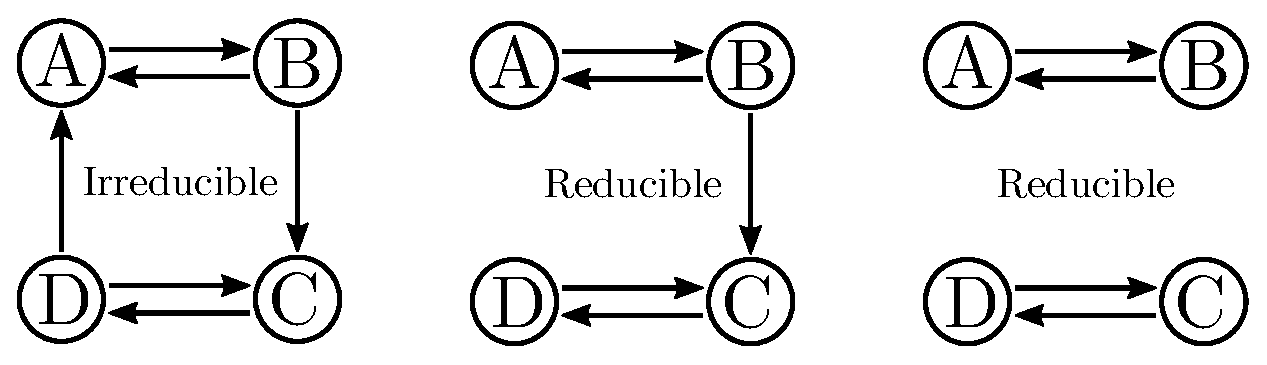
\includegraphics[width=0.7\textwidth]{sorn_markov/mc-irreducible}
        \vspace{5pt}
        \caption{In irreducible Markov chains every state is reachable in finite time, independent of the present state. The first chain on the left side fulfills this property, while the center and right chain do not. The center chain may start in $A$ or $B$, but if $C$ is reached, $A$ and $B$ are not reachable any more. In the right chain, states $A$ and $B$ are totally separated from $C$ and $D$.}
        \vspace{15pt}
        \label{fig:irreducible}
    \end{subfigure}
    \begin{subfigure}{\textwidth}
    	\centering
        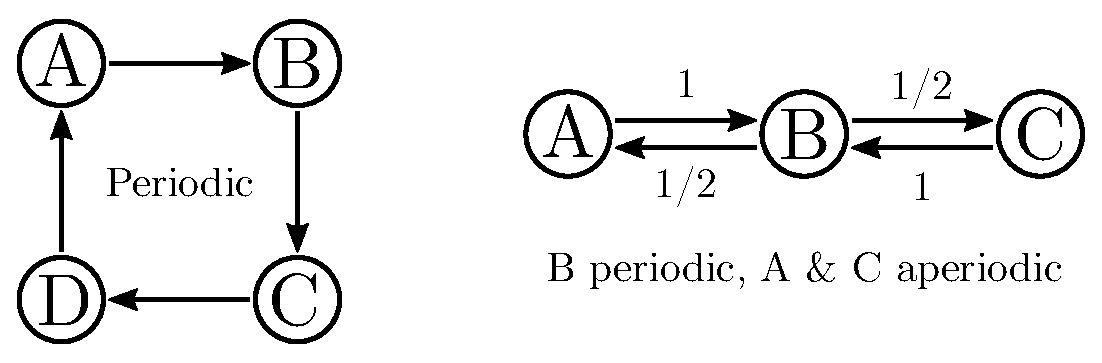
\includegraphics[width=0.7\textwidth]{sorn_markov/mc-aperiodic}
        \vspace{5pt}
        \caption{A state is periodic, if it returns back to the same state periodically, if not, the state is aperiodic. In the chain on the left side every state is periodic, since every state returns after $4$ steps. Therefore, the whole chain is periodic. On the right side, only state $B$ returns periodically every second time, states $A$ and $C$ are not periodic.}
        \vspace{15pt}
        \label{fig:aperiodic}
    \end{subfigure}
    \begin{subfigure}{\textwidth}
    	\centering
        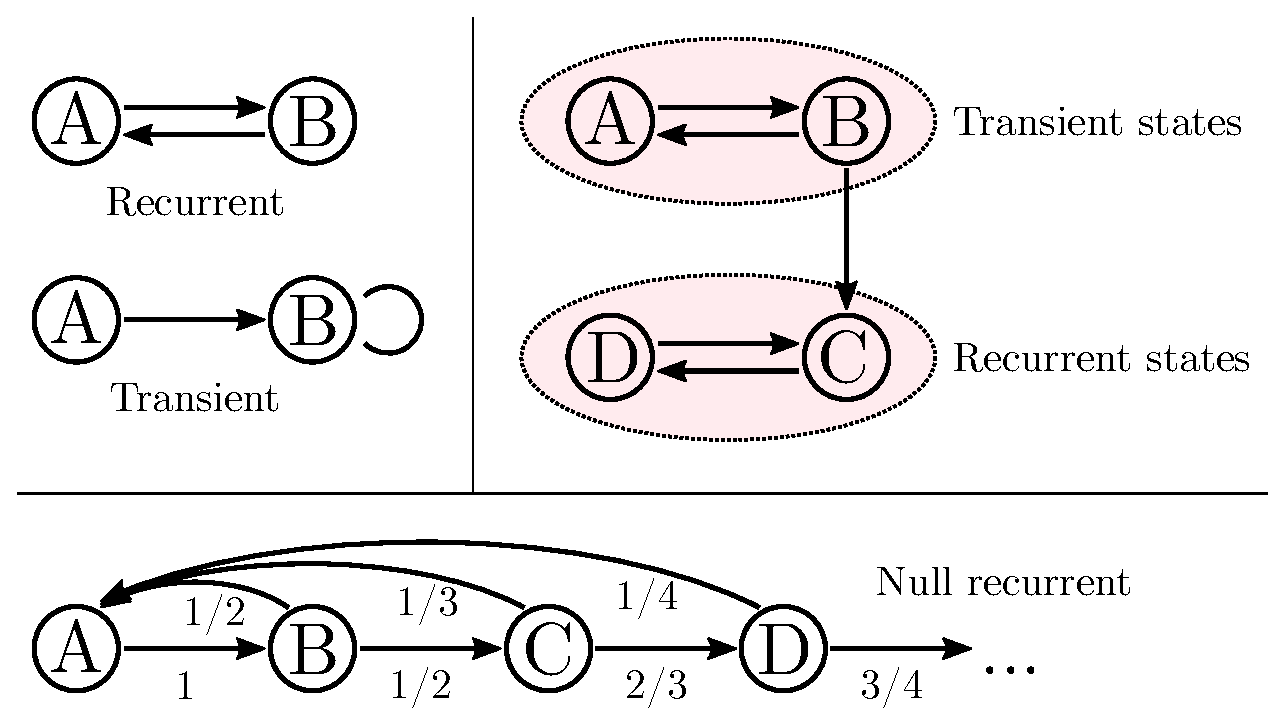
\includegraphics[width=0.7\textwidth]{sorn_markov/mc-recurrent}
        \vspace{5pt}
        \caption{If a state will be reached again almost surely, it is recurrent, otherwise transient. Two simple examples are given on top left. In the first small chain, both states $A$ and $B$ will be reached again all the time. In the second example $A$ directly goes to $B$ and will not be active any more. State $A$ is transient. On the top right, states $A$ and $B$ are transient. If $C$ is activated the first time, the chain will never reach $A$ and $B$ again. On the other hand, $C$ and $D$ are recurrent, both can be reached again all the time. The last example on the bottom shows a null recurrent case. Shown is a Markov chain with infinite states. Since the probability of going back to $A$ is decreasing with a sequence $1/n$ for $n \to\infty$, the time to go back to $A$ is $\E[T_A] = \infty$. Regarding the last chain, more details can be found in a proof in appendix in section \ref{sec:proof-null-recurrent}.}
        \label{fig:recurrent}
    \end{subfigure}
    \caption[Markov chain properties]{Three properties of Markov chains are shown: irreducibility, periodicity and recurrence. If no probability is written at an arrow, the probability is simply $p > 0$.}
    \label{fig:mc-properties}
\end{figure}

\paragraph{a) Homogeneous / Stationary Markov chain}

If the transition probabilities $p_{ij}(t)$ from state $x_i$ to state $x_j$ are independent from time $t$, i.e. $p_{ij}(t) = p_{ij}$ for all $t\in\N$, the Markov chain is called \emph{homogeneous} or stationary Markov chain. It means that

\begin{equation}
\label{eq:markov-homo}
p_{ij} = \Pb(X_{t+1} = x_j | X_t = x_i) =  \Pb(X_t = x_j | X_{t-1} = x_i).
\end{equation}

\paragraph{b) Irreducible Markov chain}

In \emph{irreducible} Markov chains, any state is reachable in finite time, independent of the present state. Formally a Markov chain is irreducible if there exists any $m < \infty$ with

\begin{equation}
\Pb(X_{t+m} = x_j | X_t = x_i) = p_{ij}^{(t+m)} > 0
\end{equation}

for all $i,j$. Examples for reducible and irreducible Markov chains are given in figure \ref{fig:irreducible}.

\paragraph{c) Aperiodic Markov chain}

If a state $x_i$ returns with a multiple of $k$ again to state $x_i$, it is called \emph{periodic}, otherwise \emph{aperiodic}. Formally a \emph{period} is defined as

\begin{equation}
k = \text{gcd} \{ t > 0\,:\,\Pb(X_t = x_i | X_0 = x_i) = p_{ii}^{(t)} > 0 \},
\end{equation}

where $\text{gcd}$ is the greatest common divisor. If the set is empty, the period is not defined. In case that $k=1$ the state $x_i$ is aperiodic and otherwise, if $k>1$, $x_i$ is periodic.

If all states are aperiodic, the Markov chain is called aperiodic. Examples for periodicity and aperiodicity are given in figure \ref{fig:aperiodic}.

\paragraph{d) Recurrent Markov chain}

A state $x_i$ of a Markov chain is called \emph{recurrent} if it  will be reached again almost surely. Therefore, the probability to come back to state $x_i$ is one. Let

\begin{equation}
\label{eq:first-comeback}
T_{x_i} = \inf\{ t \ge 0 \,:\, X_t = x_i | X_0 = x_i \}
\end{equation}

\nomenclature{$T_{x_i}$}{Number of steps until a Markov state is reached again for the first time}

be a random variable, which defines the number of steps until state $x_i$ is reached again for the first time and let $\Pb(T_{x_i} = t)$ the probability to reach $x_i$ again for the first time after exactly $t$ steps. Then state $x_i$ is recurrent, if and only if

\begin{equation}
\label{eq:recurrent}
\Pb(T_{x_i} < \infty) = \sum_{t=1}^\infty \Pb(T_{x_i} = t) = 1,
\end{equation}

If a state is not recurrent, it is called \emph{transient}, which is the case if $\Pb(T_{x_i} < \infty) < 1$. It means that the state will not be reached again almost surely.

Furthermore, if the state is recurrent and the expected value is finite, thus

\begin{equation}
\label{eq:first-comeback-expect}
\E[T_{x_i}] = \sum_{t=1}^\infty t \cdot \Pb(T_{x_i} = t) < \infty,
\end{equation}

the state is called \emph{positive recurrent}. Otherwise, if $\E[T_{x_i}] = \infty$, it is called \emph{null recurrent}.

If all states are (positive) recurrent, the Markov chain is called (positive) recurrent. Examples for recurrent and transient Markov chains are given in figure \ref{fig:recurrent}. A proof for the null recurrent chain in the figure can be found in the appendix in section \ref{sec:proof-null-recurrent}.

%%%%% Stationary %%%%%
\subsection{Stationary distribution}
\label{sec:stat-markov}

%* Definition of stationary distribution\\ 
%* Theorems about stationary distribution

\begin{definition}[Stationary distribution]

Given a homogeneous Markov chain in discrete time $t \in \N$ on state space $S = \{x_1, x_2, ...\}$, the distribution $\Pb_\pi$ is called stationary distribution if and only if

\begin{equation}
\label{eq:markov-stat}
\bm\pi_{x_j} = \Pb_\pi(X_t = x_j) = \sum_{x_i \in S} \Pb_\pi(X_t = x_i)\,p_{ij} \overset{\eqref{eq:markov-homo}}{=} \sum_{x_i \in S} \Pb_\pi(X_t = x_i)\,\Pb(X_t = x_j | X_{t-1} = x_i)
\end{equation}

for all $x_j \in S$.
\end{definition}

\nomenclature{$\bm\pi$}{Stationary distribution of a Markov chain}

The stationary distribution should not be confused with the stationary Markov chain. While the stationary Markov chain is stationary regarding the transition probabilities, the stationary distribution is stationary regarding the probability of the states. Furthermore, the presence of a stationary Markov chain (homogeneous Markov chain) is a condition for the existence of a stationary distribution.

It is not always given that a stationary distribution exists. Furthermore a stationary distribution is not necessarily unique. In the following, first, the general Perron-Frobenius-Theorem \parencite{seneta2006non, pillai2005perron} is presented. Based on this theorem, a statement about the stationary distribution can be derived. While this theorem is highly useful, it assumes aperiodic Markov chains, which are not given in any case. Hence, afterwards another theorem is introduced, which lowers the assumption. At that point I want to remind, that a \emph{homogeneous} Markov chain is assumed in the following.

\begin{definition}[Primitive matrix]
Given a squared matrix $Q = (q_{ij})_{i,j \in\N}$, it is called a primitive matrix if all items are non-negative, $q_{ij} > 0 \,\forall i,j$, denoted by $Q > 0$ and if a $k \in \N$ exists, such that all items of the matrix $Q^k$ ($k$-th power of $Q$) are positive, denoted by $Q^k > 0$.
\end{definition}

\begin{theorem}[Perron-Frobenius]
\label{eq:perron-frobenius}
Suppose $Q$ is an $n \times n$ non-negative primitive matrix. Then there exists an eigenvalue $r$, called Perron-Frobenius eigenvalue, such that:

\begin{enumerate}
\item $r$ is real and positive, $r>0$.
\item $r$ can be associated with strictly positive left and right eigenvectors.
\item $r > |\lambda|$ for any other eigenvalue $\lambda \neq r$.
\item The eigenvectors associated with $r$ are unique to constant multiples.
\item If $0 \le B \le Q$ and $\beta$ is eigenvalue of $B$, then $|\beta| \le r$. Moreover, $|\beta| = r$ implies $B = Q$.
\item $r$ is a simple root of the characteristic equation of $Q$.
\end{enumerate}
\end{theorem}

A proof is given in \textcite[Theorem 1.1]{seneta2006non}. Using the Perron-Frobenius theorem it is possible to state in which cases a unique solution for the stationary distribution can be found.

\begin{theorem}
\label{th:markov-stat}
Let $M$ be a transition matrix and $\bm 1$ a vector where all entries are one. An irreducible and aperiodic Markov chain has a unique stationary distribution given by the solution $\bm\pi$ of $\bm\pi^T M = \bm\pi^T$, where $\bm\pi^T \mathbf{1} = 1$.
\end{theorem}

This theorem will be proven, but two corollaries are necessary.

\begin{corollary}
\label{co:primitive}
An irreducible and aperiodic matrix is primitive.
\end{corollary}

\begin{corollary}
\label{co:smallest-largest}
Let $Q$ be a positive square matrix. Then the minimal row sum is a lower bound and the maximal row sum is an upper bound of the the largest eigenvalue of $Q$.
\end{corollary}

\begin{proof}[Proof for theorem \ref{th:markov-stat}]
Since any transition matrix $M$ is per definition square and non-negative, the statements of the Perron-Frobenius theorem hold for transition matrix $M$, if the Markov chain is primitive. Since corollary \ref{co:primitive} states that any irreducible and aperiodic matrix is primitive, the assumptions of the theorem are clarified.

Furthermore, it holds that

\begin{equation*}
M\mathbf{1} = \mathbf{1},
\end{equation*}

since every row sums to one by definition of the transition matrix. Hence, $M$ has an eigenvalue of $1$ and an eigenvector of $\mathbf{1}$. With corollary \ref{co:smallest-largest}, the largest eigenvalue is exactly the row sum $1$, since all rows of $M$ have the same sum. Therefore, the eigenvalue $r=1$ is the Perron-Frobenius eigenvalue, since property (3) of the theorem states that all other eigenvalues are smaller in absolute. The corresponding right Perron-Frobenius eigenvector is $\mathbf{1}$.

Assuming that a vector $\bm v^T$ is normed, such that $\bm v^T \mathbf{1} = 1$, the eigenvalue problem for the left eigenvector $\bm v^T$ has the following form:

\begin{equation*}
\bm v^T M = r \bm v^T = \bm v^T
\end{equation*}

From statement (2), we know that the left eigenvector regarding $r$ is strictly positive. Therefore, $\bm v^T = \bm\pi^T$ is a distribution, the stationary distribution.

Finally, statement (4) of the Perron-Frobenius theorem states that $\bm\pi$ is unique.
\end{proof}

As a side note, using theorem \ref{th:markov-stat}, the stationary distribution can be calculated as a right eigenvalue problem, just by transposing both sides $(\bm\pi^T M)^T = (\bm\pi^T)^T$, which results in $M^T \bm\pi = \bm\pi$.

Theorem \ref{th:markov-stat} is limited to aperiodic Markov chains. Another theorem lowers the assumptions.

\begin{theorem}
\label{th:irr-rec}
An irreducible and positive recurrent Markov chain has a unique stationary distribution $\bm\pi$ given by

\begin{equation}
\pi_{x_i} = \frac{1}{\E[T_{x_i}]}
\end{equation}
\end{theorem}

A proof is given in \textcite[Corollary 1.2.29]{bladt2017matrix}. The theorem uses the definition of the random variable $T_{x_i}$ from equation \eqref{eq:first-comeback}, which indicates the number of steps, necessary to come back to state $x_i$ again for the first time. Furthermore $\E[T_{x_i}]$ was defined in equation \eqref{eq:first-comeback-expect}.

\begin{theorem}
An irreducible and finite Markov chain is positive recurrent.
\end{theorem}

This theorem is proven in \textcite[Theorem 3.3]{bremaud2013markov}. It shows, that theorem \ref{th:irr-rec} is highly practical for finite Markov chains. Since, in case of finite Markov chains, only the property of irreducibility needs to be fulfilled.

The Perron-Frobenius theorem has a slight advantage, compared to theorem \ref{th:irr-rec}. Using the Perron-Frobenius theorem, it can be shown that even a \emph{limiting distribution} can be obtained. It is defined by $\pi_i = \lim_{t \to\infty} \Pb(X_t = x_i)$. In case of theorem \ref{th:irr-rec}, this is not necessarily the case. If we assume for example a periodic Markov chain with just two states, which are alternating $(0,1,0,1,0,1, ...)$, the Markov chain has no limiting distribution, but a unique stationary distribution. However, for calculating stationary distributions, in most cases theorem \ref{th:markov-stat} was used.

%%%%% Measures %%%%%
\subsection{Measures}
\label{sec:markov-measures}

To evaluate the stationary distribution many measures can be used, which are common for any distribution, not only for Markov chains. Two types are introduced, which are used in the results. At first, information measures, namely variance and Kullback-Leibler divergence, are defined and afterwards a measure for the concentration of a distribution is presented, where the Lorenz curve and the Gini coefficient are introduced. Note that the Gini coefficient is directly derived from the Lorenz curve.

\paragraph{Information measures}

For simplification, the state space can be defined as $S = \{1, ..., n\}$ where $n \in\N$. A simple measure for the stationary distribution is the deviation of the probabilities from their mean probability. Therefore an empirical variance measure is used by calculating

\begin{equation}
\label{eq:variance-estimate}
\sigma^2_\pi = \frac{1}{n} \sum_{k=1}^n (\pi_k - \bar\pi)^2,
\end{equation}

where $\bar\pi = \frac{1}{n} \sum_{k=1}^n \pi_k$. In the following it is just called \emph{variance}.

% If $\Pi = (\Pi_1, ..., \Pi_n)^T$ denotes a random variable for the stationary distribution, the variance of the stationary distribution is given by

% \begin{equation}
% \label{eq:variance}
% \Var(\Pi) = \E[(\Pi - \E[\Pi])^T (\Pi - \E[\Pi])],
% \end{equation}

% which can be interpreted as the expected squared distances between the probabilities of the stationary distribution and their expectation value.

% Since the random variable $\Pi$ depends on the stochastic transition matrix, with probabilities $\Pb(X_{t+1} = x_i | X_t = x_j)$, where $X_t$ is the random variable of the current state at time $t$, it is not easy to obtain the variance analytically. Therefore, a simple estimator is suggested, defined by

% \begin{equation}
% \label{eq:variance-estimate}
% \widehat{\Var(\Pi)} = \sigma^2_\pi = \sum_{k=1}^n (\pi_k - \bar\pi)^2,
% \end{equation}

% where $\bar\pi = \frac{1}{n} \sum_{k=1}^n \pi_k$.

Another measure uses the Kullback-Leibler divergence. If $\bm\pi' \in \{\pi'_1, ..., \pi'_n\} = \{1/n, ..., 1/n\}$ is a stationary distribution where all states are equally probable, the Kullback-Leibler divergence can be obtained by

\begin{equation}
\label{eq:kullbackleibler}
\DKL = \sum_{i=1}^n \pi_i \ln{\left(\frac{\pi_i}{\pi'_i}\right)}.
\end{equation}

The Kullback-Leibler divergence can be understood as relative entropy. It describes the increase in information which is necessary to describe $\bm\pi$, when $\bm\pi'$ is given. It is important to note that the Kullback-Leibler divergence is an asymmetric measure. The value of the measure depends on the order of the distributions and therefore the divergence does not fulfill the properties of a \emph{metric}. It is in particular different from the \emph{total variation distance} $\delta(\bm\pi, \bm\pi')$. A link between the total variation distance and the Kullback-Leibler divergence is given by \emph{Pinsker's inequality}. However, \emph{Gibb's inequality} states that

\begin{equation}
\label{eq:kullbackleibler-gibbs}
\DKL \ge 0
\end{equation}

and $\DKL = 0$ if and only if $\bm\pi = \bm\pi'$, which means that a divergence of $0$ indicates a match between the distributions $\bm\pi$ and $\bm\pi'$.

\begin{SCfigure}[0.6][!b]
    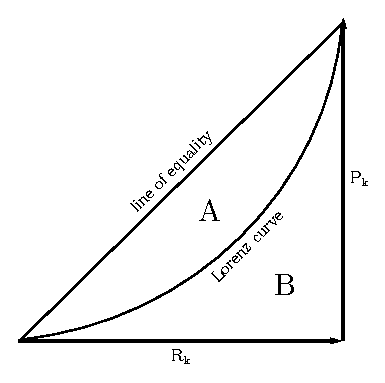
\includegraphics[width=0.45\textwidth]{sorn_markov/lorenz}
    \caption[Lorenz curve]{Illustration of a Lorenz curve. On the $x$-axis is the cumulative share of the probabilities from the states of an equally distributed stationary distribution. On the $y$-axis is the cumulative share of the probabilities of the actual stationary distribution. If the actual distribution is equally distributed, the Lorenz curve reaches the line of equality. The Gini coefficient is calculated by $G = A / (A+B)$.}
    \label{fig:lorenz-illustration}
\end{SCfigure}

\paragraph{Concentration measures}

Another way of evaluating the properties of a Markov chain is to plot the \emph{Lorenz curve} and calculate the \emph{Gini coefficient}. Traditionally, both is often applied to indicate inequality regarding income, used in social sciences. But the Lorenz curve shows the concentration of a distribution in general, whereas the Gini coefficient is a related measure for the intensity of the concentration of the given distribution.

First, assume that $\bm\pi = (\pi_1, ..., \pi_n)^T$ is sorted in a sense that $\pi_1 \le ... \le \pi_n$ and denote $r_i = 1/n$ as the share of a state with probability $\pi_i$, where $n\in\N$ is the number of states. Furthermore $R_k = \sum_{i=1}^k r_i = \sum_{i=1}^k 1/n = k/n$ is the cumulative share of the states. On the other hand, $P_k = \sum_{i=1}^k \pi_i$ is the cumulated probability of $\bm\pi$. The \emph{Lorenz curve} shows the cumulated share of states $R_k$ at the $x$-axis and the cumulated probability $P_k$ at the $y$-axis. If all probabilities are equal, it will result in a straight diagonal line. The more the distribution $\bm\pi$ is concentrated, the more the line will appear in the right bottom corner. An illustration is given in figure \ref{fig:lorenz-illustration}.

Finally, the \emph{Gini coefficient} $G$ is the ratio of the area that lies between the diagonal line, where all states are equal probable, and the area between the actual Lorenz curve and the diagonal. The more the Lorenz curve tends to the corner and, therefore, the more the stationary distribution is unequal, the more the Gini coefficient will tend to $1$, where $1$ represents a perfect concentrated situation. It means that the whole probability is concentrated at one state, the other states are zero. If the distribution is perfectly equal, the Gini coefficient will reach $0$. It can be shown that $G \in [0,1]$ is half of the \emph{relative mean absolute difference}. Hence, for the discrete case, the Gini coefficient is defined as

\begin{equation}
\label{eq:gini}
G = \frac{\sum_{i=1}^n \sum_{j=1}^n |\pi_i - \pi_j|}{2n\cdot \sum_{i=1}^n \pi_i}.
\end{equation}

%%%%% Monte Carlo %%%%%
\subsection{Markov Chain Monte Carlo (MCMC)}

A \emph{Monte Carlo simulation} is a stochastic procedure where random samples are drawn many times. As a result, numerical solutions for analytically difficult or even impossible problems are obtained. \textcite{thomopoulos2012essentials} described the process as follows:

\begin{quote}
To apply the Monte Carlo method, the analyst constructs a mathematical model that simulates a real system. A large number of random sampling of the model is applied yielding a large number of random samples of output results from the model.
\end{quote}

Specifically, if random samples are drawn from the distribution of a Markov chain, it is called \acfi{mcmc} method which includes a broad class of algorithms. Famous and well known algorithms are the \emph{Metropolis–Hastings algorithm} \parencite{hastings1970monte} or the \emph{Gibbs sampler} \parencite{geman1984stochastic}. These techniques are often used in Bayesian inference to evaluate posterior distributions.

There are many different possibilities to understand the behavior of neural networks under the perspective of \acs{mcmc} sampling. For example, there are applications for Boltzmann machines \parencite{osogami2017boltzmann} or energy-based models in general \parencite{goodfellow2007deep}. In \acs{sorn}, it is possible to view the learned time-dependent input patterns under the perspective of \acs{mcmc} sampling. The approach will be introduced in methods (section \ref{sec:methods}) and many illustrative implementations will be given in results (section \ref{sec:results}).

%%%%% MCMC / ANN %%%%%
%\subsection{MCMC and neural networks}

%An overview to MCMC methods in neural networks is given in \cite{andrieu2003introduction}.

%Boltzmann machines, which are a special kind of a stochastic recurrent neural networks, highly depend on a MCMC approach. They are trained by stochastic gradient, where expected values need to be calculated. In many cases those expected values cannot be calculated analytically. Therefore MCMC methods, especially Gibbs sampling can be used to finally train Boltzmann machines \parencite{osogami2017boltzmann}. The MCMC approach can also be used for the broader class of energy-based models \parencite{goodfellow2007deep}.

%MCMC can also be used for model selection. It can for example applied to estimate the number of neurons in a network (3 citations).
% http://www.cs.ubc.ca/~arnaud/andrieu_defreitas_doucet_jordan_intromontecarlomachinelearning.pdf (Seite 23)

%Sampling Maas / Sampling perspective

%It can be summarized that MCMC plays an important role in specific applications of neural networks. The last application should be kept in mind, since in methods section another perspective is introduced, which is inspired by the approach of (paper Maas).

%Where was it used in literature before? link to neural networks?

%Introduce perspective to SORN networks -> In methods





















\section{Methods}
\label{sec:methods}

A self-organizing recurrent neural network (SORN) was used to learn specific input patterns, given by a defined Markov chain. It was checked how well the network was able to represent the given information. \acs{sorn} uses three plasticity rules to learn the input patterns:

\begin{itemize}
\item \ACF{stdp}
\item \ACF{sn}
\item \ACF{ip}
\end{itemize}

The time in the network is discrete and there is no refractory period modeled for the neurons. In most cases $\Nsim = 20$ networks were simulated and results were averaged.

% Zitiere grand averaging paper

The source code for all the simulation experiments is based on source code from \textcite{hartmann2015s}, which is written in \texttt{Python 2.7}. The team provided a small framework for SORN simulation experiments (\href{https://github.com/chrhartm/SORN}{https://github.com/chrhartm/SORN}). A lot of code was added or rewritten, especially regarding the evaluation of the network behavior, such that it fitted to the experiments, performed in this thesis.

\subsection{Network structure}

The reservoir consists of $N^E$ excitatory and $N^I$ inhibitory neurons. Additionally, some excitatory neurons where randomly connected to a specific number of input neurons $N^U = n$, which equals the number of Markov states. The weights $w_{ij} \in [0,1]$ between the neurons were initialized randomly. The network is build with three types of connections:

\begin{itemize}
\item Excitatory-excitatory weights: $W^{EE}$, where $\sum_{j} w^{EE}_{ij} = 1$
\item Inhibitory-excitatory weights: $W^{EI}$, where $\sum_{j} w^{EI}_{ij} = 1$
\item Excitatory-inhibitory weights: $W^{IE}$, where $\sum_{j} w^{IE}_{ij} = 1$
\item Input-excitatory weights: $W^{EU}$, where $w^{EU}_{ij} = 1$ for all $i,j$
\end{itemize}

As already explained in section \ref{sec:sorn}, there are no connections modeled between inhibitory neurons. On average, $10\%$ of the possible connections in $W^{EE}$ were realized. Hence, the matrix $W^{EE}$ is sparsely connected. The matrices $W^{IE}$ and $W^{EI}$ are fully connected. Note that the weights are normalized using equation \eqref{eq:sn}, such that the incoming weights to a neuron sum up to one.

In section \ref{sec:sorn}, figure \ref{fig:sorn} shows a sketch of the structure of the reservoir network. In this thesis $n = 4$ states were used. Hence, the state space consists of $S = \{x_1, x_2, x_3, x_4\} = \{A, B, C, D\}$. Three states are no enough to test a variety of combinations, while five or more states are already to complicated for a systematic approach. Therefore, four states seemed to be a good compromise. The four states are represented with neuron populations, called clusters. In most cases the network consists of $N^E = 200$ and $N^I = 40$. Furthermore $N_{x_i}^U = 10$ input connections are used per state or input neuron.

\subsection{Modification of the intrinsic plasticity}
\label{sec:ip-mod}

While the \acs{stdp} and the \acs{sn} where applied analog to \textcite{lazar2009sorn}, the \acs{ip} rule was modified. In the original \acs{sorn} model, the target rate $H_\IP$ was fixed. \textcite{hartmann2015s} found out that the model is more robust, if the average firing rate differs slightly between neurons. Therefore, the $H_\IP$ value from equation \eqref{eq:ip} was replaced by an individual $H_i^\IP$ target rate for every neuron $i$, resulting in

\begin{equation}
\label{eq:ip-ind}
T_i(t+1) = T_i(t) + \eta_\IP \left( x_i(t) - H_i^\IP \right).
\end{equation}

To get individual values, an average value $\bar H_\IP = 2\cdot N^U/N^E$ was used. It equals the original heuristic from \textcite{lazar2009sorn}. Additionally, a stochastic term $\varepsilon_i^\IP$ was added to the target rate of every neuron. It is uniformly \acs{iid} on an interval of $a = \sigma^\IP = 0.01$ and $b = -a = -\sigma^\IP = -0.01$. Therefore, $\varepsilon_i^\IP \sim \text{Uni}[a,b] = \text{Uni}[-\sigma^\IP,+\sigma^\IP] = \text{Uni}[-0.01,0.01]$. Together,

\begin{equation}
\label{eq:hip-ind}
T_i(t+1) = T_i(t) + \eta_\IP \left( x_i(t) - \bar H^\IP + \varepsilon_i^\IP \right)
\end{equation}

\nomenclature{$\bar H^\IP$}{Average target rate of IP mechanism}
\nomenclature{$\sigma^\IP$}{Target rate range of IP mechanism}

is the rule that was applied in the used network.

\subsection{Network training and testing}
\label{sec:train}

The network was trained in 3 phases:

\begin{itemize}
\item Self-organizing phase (plastic training phase)
\item Training phase (no-plastic training phase)
\item Testing phase
\end{itemize}

\paragraph{Self-organizing phase}

In the self-organizing phase (or plastic training phase) the input neurons are active, depending on the current sample $x_i$ from the Markov chain. In this phase all three plasticity rules are active. While STDP actively adjusts the weights, SN stabilizes the activity around every neuron without loosing the relative relationships between the neurons. IP also helps to ensure the stability of the network, since it adjusts thresholds of neurons depending on their past activity. The update of the network activity follows equation \eqref{eq:update-excitatory} for the excitatory neurons and equation \eqref{eq:update-inhibitory} for the inhibitory neurons.

During self-organizing, the information from the Markov chain is stored in the network and is coded in the weights between the neurons. Biologically, the encoding in the weights corresponds to the encoding in the strength of the synapses. In most cases the self-organizing phase was applied for $T_\plastic = 50,000$ steps. As shown below in the results, e.g. in figure \ref{fig:mc1-training}, latest after $50,000$ steps no further improvement can be noticed, in most cases much sooner.

\paragraph{Training phase}

In the training phase (or no-plastic training phase) the input neurons are still active and they still depend on the current state $x_i$ of the Markov chain. In this phase only \ac{ip} is active. Therefore, the stability of the network is ensured further on. \ac{stdp} is not active and thus also \ac{sn} is not necessary. Hence, the weights stay fixed in the training phase, meaning that $W^{EE}_{ij}(t) = W^{EE}_{ij}$ in equation \eqref{eq:update-excitatory}, where the rest of the network update equals the self-organizing phase.

The main role of the training phase is to find out how the states are represented in the activity patterns of the network after the weight structure was learned. After a burn in phase, \textcite{hartmann2015s} used the last $\tilde{T}_\compare = 2500$ steps of the no-plastic training phase for classification (see section \ref{sec:state-classification}). In the results section, it is shown that this fixed value causes a small bias, which was solved when choosing $\tilde{T}_{\text{compare}}$ more flexible, which is explained below in section \ref{sec:state-classification}.

The training phase needs enough steps to cover $\Tnoplastic > \tilde{T}_\compare$. However, the training was mostly chosen as $\Tnoplastic = 50,000$ no-plastic training steps. There are four reasons for this high value:

\begin{itemize}
\item The computational effort is very low in the training phase.
\item The number of no-plastic training steps do not influence the performance of the network (see appendix \ref{sec:appendix:noplastic}).
\item After switching off the self-organizing phase (namely the \ac{stdp} and \ac{sn}), there should be a short burn-in period. \textcite{hartmann2015s} used $\Tnoplastic = 20,000$, which seemed to be enough in all cases.
\item The updated classification algorithm, mentioned above, implies a flexible size of $\tilde{T}_\compare$, depending on the Markov chain. This change caused that a longer training phase is necessary in some cases. $\Tnoplastic = 50,000$ was enough for all applications.
\end{itemize}

\paragraph{Testing phase}

In the testing phase the input neurons are not active any more, there is no input at all. It means that $\bm v(t) = 0$ for all $t \in \{\Tevo+1, ..., \Tevo+\Ttest\}$, where $\Tevo = T_\plastic + \Tnoplastic$. Also \ac{stdp} and \ac{sn} is still switched off, as it was in the training phase before. \ac{ip} is still active. Beside the stabilizing character of the \acs{ip}, especially in the testing phase, it is responsible for spontaneous activity (see section \ref{sec:ip}). In the testing phase, the spontaneous activity patterns of the network are observed over time.

Since no input is given in this phase, it is necessary to classify the spontaneous activity patterns to a Markov state. For that purpose, the representations from the no-plastic training phase are used. A detailed explanation of the classification mechanism is given below.

The number of steps while testing has to take into account a short period of burn in. After the training phase, the input is switched off and therefore the network has to find equilibrium again, using just spontaneous activity from \acl{ip}. Mathematically, the burn in time depends on the learning rate of the \acs{ip} mechanism $\eta_\IP$. This relation is evaluated in appendix \ref{sec:appendix:eta}. In most cases the burn in phase is relatively short and $\Ttest > 20,000$ is sufficient.

\subsection{Classification of states}
\label{sec:state-classification}

In the last phase, the testing phase, it will be necessary to classify a Markov state $x_i$ to the activity pattern $\bm x(t)$ in every step of time. The activity patterns from the testing phase are compared to some representative activity patterns in the end of the no-plastic training phase.

\paragraph{Selection mechanism from Hartmann}

In \textcite{hartmann2015s} a fixed amount of $\tilde{T}_\compare = 2500$ steps in the training phase was used as representative activity patterns. From those steps the number of occurrences for every state $\tilde{T}_\compare^{x_i}$ was calculated. Let

\begin{equation}
\begin{split}
\tilde{R}_\compare &= \left\{ \bm x_u(T_\plastic+T_\noplastic-\tilde{T}_\compare), ..., \bm x_u(T_\plastic+T_\noplastic) \right\}\\
&= \left\{ \bm x_u(T_\evo-\tilde{T}_\compare), ..., \bm x_u(T_\evo) \right\}
\end{split}
\end{equation}

be a set of the last $\tilde{T}_\compare$ activity patterns in the no-plastic phase, where $u \in \{x_1, ..., x_n\}$ indicates the given input for the specific step. In order to avoid confusion, it is important to remind that the vector $\bm x_u(t)$ denotes the activity pattern of the excitatory neurons at time $t$ with input $u$ and the scalar $x_i$ denotes a state of the Markov chain. The obtained activity patterns $\tilde{R}_\compare$ are filtered by Markov state, denoted by $\tilde{R}_\compare^{x_i} = \{ \tilde{R}_\compare | u = x_i \}$. The size of this set is defined as $\tilde{T}_\compare^{x_i} = |\tilde{R}_\compare^{x_i}|$, which was mentioned above.

The minimum of those occurrences $T_\compare^\mini = \min\{\tilde{T}_\compare^{x_1}, ..., \tilde{T}_\compare^{x_n}\}$ was chosen as the number of steps for every state. If the number of representative activity patterns per state would differ, those with a higher amount of steps have a higher chance to be classified, since the amount of representative patterns cover more possible cases. Altogether, $n \cdot T_\compare^\mini$ steps are available for comparison, where $n$ is the number of Markov states or input neurons. The corresponding activity pattern for a specific state is denoted by $R_\compare^{x_i}$. To clarify how it works, a short example is provided:

Assume just two possible states $A$ and $B$, thus $n=2$. Further, assume that a Markov chain exists which provides a stationary distribution with $\pi_A = 2/5$ and $\pi_B = 3/5$. A likely sampling would result in $\tilde{T}_\compare^A = 997$ (where $\tilde{T}_\compare \cdot \pi_A = 2500 \cdot 2/5 = 1000$ would be expected) and $\tilde{T}_\compare^B = 1503$ (where $\tilde{T}_\compare \cdot \pi_B = 1500$ would be expected). Finally, in testing phase are more representative activity patterns of $B$ than $A$ available to compare with. Hence, $B$ has an advantage, compared to $A$, and activity patterns in the testing state will eventually more likely be classified as $B$. To avoid this possible bias, the minimum of both values is taken and $T_\compare^\mini = \min\{\tilde{T}_\compare^A, \tilde{T}_\compare^B\} = \min\{997,1503\} = 997$ is the number of steps which are used for \emph{every} state to compare with, meaning that $T_\compare^\mini = T_\compare^A = T_\compare^B$. Figure \ref{fig:classification-old} illustrates a similar example.

\begin{figure}
    \centering
    \begin{subfigure}{\textwidth}
    	\centering
        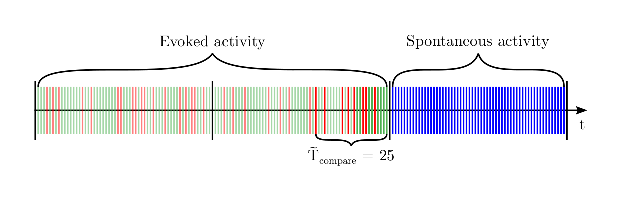
\includegraphics[width=\textwidth]{methods/classification_old}
        \vspace{5pt}
        \caption{A fixed number of potential activity patterns is chosen. In this example $\tilde{T}_\compare = 25$, meaning that the last $25$ steps in time are taken into account. In this period, state $A$ occurs $\tilde{T}_\compare^A = 8$ times and state $B$ $\tilde{T}_\compare^B = 17$ times. To ensure that the later classification of the spontaneous activity pattern have the same chance to be classified, $T_\compare^\mini = T_\compare^A = T_\compare^B = 8$ is chosen for both, state $A$ and $B$.}
        \vspace{20pt}
        \label{fig:classification-old}
    \end{subfigure}
    \begin{subfigure}{\textwidth}
    	\centering
        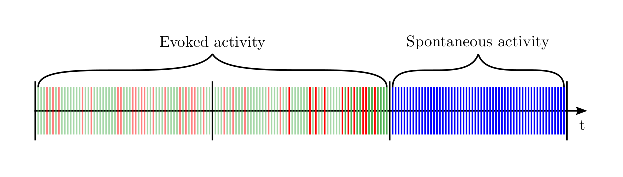
\includegraphics[width=\textwidth]{methods/classification_new}
        \vspace{5pt}
        \caption{Since the $T_\compare^\mini$ from the solution from \textcite{hartmann2015s} varies between input patterns with different probabilities, another bias needs to be taken into account when different learning patterns should be compared. Therefore, independent of the probability structure, $T_\compare = T_\compare^A = T_\compare^B = 10$ are chosen for all states. The search for those states begins at the end of the no-plastic training phase.}
        \vspace{20pt}
        \label{fig:classification-new}
    \end{subfigure}
    \caption[Selection mechanism for activity pattern representations]{Selection mechanism for activity pattern representations. In both illustrations, the first block is the plastic training phase, the second block represents the no-plastic training phase and the last block is the testing phase. Since input is given in the first two blocks, they perform with evoked activity. The last block has no input anymore and runs only with spontaneous activity from \acs{ip}. The example network is trained with two states: $A$, represented by the red lines, and $B$, drawn in green, where $\pi_A = 2/5$ and $\pi_B = 3/5$. Every line represents a point in time. The opaque lines are the selected steps, which are used as representative activity patterns for the specific state of the Markov chain. The activity of the chosen steps is collected in $R_\compare$ in general and in $R_\compare^A$ \& $R_\compare^B$ specifically. The first graphic shows the method provided by \textcite{hartmann2015s}, the second graphic illustrates the method which is applied in the network of this thesis.}
    \label{fig:classification}
\end{figure}

\paragraph{Updated selection mechanism}

While evaluating the network, another bias was found. The algorithm from \textcite{hartmann2015s} makes sure that the classification remains unbiased, if the same input pattern is chosen. But if different patterns are compared, the classification mechanism depends on the probabilities of the states. If one state in the input pattern is very rare, $T_\compare^\mini$ will be very small and therefore all activity patterns in the testing phase have just few representative patterns in the no-plastic training phase to compare with. On the other hand, if all states are equally probable, $T_\compare^\mini$ is quite high compared to the rare case. The performance between those two cases will eventually differ, just because of the number of available representative states in no-plastic training phase. In terms of Markov chains: If Markov chains with different stationary distributions are learned by the network and compared with each other, it is necessary to keep the number of $T_\compare^\mini$ constant for all chains. In section \ref{sec:input-dep-per} this effect is illustrated and discussed in detail.

An approach, which was chosen in this thesis, is to fix the number of representing steps for every state. A value of $T_\compare = 500$ was chosen. Independent of the probability of the state, starting from the end, $500$ representing activity patterns for every state were collected. If a state is very unlikely, for example with a probability of $\pi_{x_i} = 0.05$, for $500$ occurrences, $10,000$ steps are necessary in average to find enough representations for that state. Therefore, the $\Tnoplastic = 50,000$ was chosen, as indicated before. An illustration of this selection mechanism is shown in figure \ref{fig:classification-new}.

\paragraph{Classification mechanism}

After the representational activity patterns $R_\compare$ are collected with equal length $T_\compare^{x_1} = ... = T_\compare^{x_n}$, independent of the probabilities of the Markov chain, it remains to describe the classification mechanism for the activity patterns in the testing phase. First, a distance measure, the \emph{Hamming distance} is defined.

\begin{definition}[Hamming Distance]
Let $\Omega$ be an alphabet and $\bm x = (x_1, ..., x_N) \in \Omega^N$, $\bm y = (y_1, ..., y_N) \in \Omega^N$ two words with length $N \in \N$. Then the \emph{hamming distance} between those words $\bm x$ and $\bm y$ is defined as:

\begin{equation}
\label{eq:hamming}
d(\bm x, \bm y) := |\{i \in \{1, ..., N\} : x_i \neq y_i\}|
\end{equation}
\end{definition}

For the network holds that $\Omega = \{0,1\}$. The Hamming distances between every step in the testing phase $\bm x(t_\test) \in R_\test$, where $R_\test = \{ x(T_\evo + 1), ..., x(T_\evo + T_\test) \}$, and all steps in $\bm x(t_\compare) \in R_\compare$  are calculated. In that case the Hamming distance is defined as

\begin{equation}
\label{eq:hamming-applied}
d(\bm x(t_\test), \bm x(t_\compare)) = |\{ i \in \{ 1, ..., N^E \} : x_i(t_\test) \neq  x_i(t_\compare) \}|.
\end{equation}

\begin{table}[!b]
\centering
\footnotesize
\begin{tabular}{l|llllllllll|c}
$x_i$ & \multicolumn{10}{c|}{$\bm x(t_\compare)$} & $d\left(\bm x(t_\test), \bm x(t_\compare) \right)$ \\
\hline
A & \textbf{1} & \textbf{0} & 0 & \textbf{0} & \textbf{1} & 0 & \textbf{0} & 0 & \textbf{1} & 0 & 6 \\
A & 0 & \textbf{0} & 0 & \textbf{0} & 0 & \textbf{1} & \textbf{0} & \textbf{1} & 0 & \textbf{1} & 6 \\
A & 0 & 1 & 0 & \textbf{0} & 0 & \textbf{1} & \textbf{0} & \textbf{1} & \textbf{1} & 0 & 5 \\
A & 0 & \textbf{0} & \textbf{1} & \textbf{0} & 0 & \textbf{1} & 1 & 0 & \textbf{1} & \textbf{1} & 6 \\
A & 0 & \textbf{0} & 0 & 1 & 0 & 0 & \textbf{0} & \textbf{1} & \textbf{1} & \textbf{1} & 5 \\
B & 0 & 1 & \textbf{1} & \textbf{0} & 0 & 0 & 1 & 0 & 0 & 0 & 2 \\
A & 0 & 1 & 0 & 1 & 0 & \textbf{1} & \textbf{0} & \textbf{1} & \textbf{1} & \textbf{1} & 6 \\
B & 0 & 1 & \textbf{1} & 1 & 0 & 0 & \textbf{0} & 0 & 0 & 0 & 2 \\
A & \textbf{1} & \textbf{0} & 0 & \textbf{0} & 0 & \textbf{1} & 1 & \textbf{1} & \textbf{1} & \textbf{1} & 6 \\
B & \textbf{1} & 1 & \textbf{1} & 1 & 0 & 0 & 1 & 0 & 0 & \textbf{1} & 2 \\
B & 0 & \textbf{0} & \textbf{1} & 1 & 0 & 0 & \textbf{0} & 0 & 0 & 0 & 3 \\
A & \textbf{1} & 1 & 0 & \textbf{0} & 0 & 0 & 1 & \textbf{1} & \textbf{1} & \textbf{1} & 5 \\
A & 0 & \textbf{0} & 0 & \textbf{0} & 0 & \textbf{1} & \textbf{0} & \textbf{1} & \textbf{1} & \textbf{1} & 7 \\
B & 0 & 1 & \textbf{1} & 1 & 0 & 0 & 1 & 0 & 0 & 0 & \textbf{1} \\
B & 0 & 1 & \textbf{1} & \textbf{0} & 0 & 0 & \textbf{0} & \textbf{1} & \textbf{1} & 0 & 5 \\
A & 0 & \textbf{0} & 0 & \textbf{0} & 0 & 0 & \textbf{0} & 0 & 0 & \textbf{1} & 4 \\
B & 0 & \textbf{0} & \textbf{1} & 1 & 0 & 0 & \textbf{0} & 0 & 0 & 0 & 3 \\
B & \textbf{1} & 1 & \textbf{1} & 1 & 0 & 0 & \textbf{0} & \textbf{1} & 0 & 0 & 4 \\
B & 0 & 1 & \textbf{1} & 1 & 0 & 0 & \textbf{0} & \textbf{1} & 0 & 0 & 3 \\
B & 0 & \textbf{0} & 0 & 1 & 0 & 0 & 1 & 0 & 0 & 0 & \textbf{1} \\
\hline
\hline
$\bm x(t_\test)$ & 0 & 1 & 0 & 1 & 0 & 0 & 1 & 0 & 0 & 0 &  \\
\hline
$\bm u_A$ & 0 & 0 & 0 & 0 & 0 & 1 & 0 & 1 & 1 & 1 &  \\
$\bm u_B$ & 0 & 1 & 1 & 1 & 0 & 0 & 1 & 0 & 0 & 0 & 
\end{tabular}
\vspace{5pt}
\caption[State classification using Hamming distance]{State classification using Hamming distance. Shown are $T_\compare^A = T_\compare^B = 10$ representative states from the no-plastic training phase, corresponding to figure \ref{fig:classification-new}. An activity vector $\bm x(t_\test)$ and examples of input vectors $\bm u_A$ and $\bm u_B$, corresponding to the Markov states $A$ and $B$ are shown in the bottom of the table. On the right side the Hamming distance between any $\bm x(t_\compare)$ and the $\bm x(t_\test)$ is calculated. The differing digits in the vectors are bold. The smallest distance is given by two vectors corresponding to an $B$ input, with a distance of just $1$, which is highlighted in bold on the right side. Therefore, the chosen step in testing phase would be classified as $B$. This procedure is repeated for every $\bm x(t_\test) \in R_\test$.}
\label{tb:hamming}
\end{table}

The activity pattern $\bm x(t_\compare)$ with the smallest distance $d(\bm x(t_\test), \bm x(t_\compare))$ for all $t_\compare$ is chosen and denoted by $\bm x^\mini_\compare(t_\test)$. Corresponding to $\bm x^\mini_\compare(t_\test)$ exists a specific input $u \in \{x_1, ..., x_n\}$ which is chosen as the Markov state for the corresponding step $t_\test$ in the testing phase. A simple example, which gives an intuition is shown in table \ref{tb:hamming}. The process is in principle a $k$-nearest neighbors algorithm with $k=1$, where the distance between the vectors is measured using a hamming distance.

The question arises what happens if two or more patterns from training phase having equal distances, assuming that the patterns in the training phase belong to different Markov states. \textcite{hartmann2015s} solved this problem by shuffling the training states, before calculating the distances and then taking the first element which has minimum distance. With this method a systematical bias is prevented.

However, the algorithm is relatively simple, which is its strength, at least regarding computational effort and simplicity in implementation. The classification method will be examined in the results and further discussed in the discussion.

\subsection{Measuring performance}

The reservoir network is trained with a specific Markov chain, where the states in the Markov chain represent input clusters in the neural network, modeled by input neurons. Ideally, the network finds a good representation of the transition probabilities and the stationary distribution, stored in the weights, to reproduce the Markov chain. Statistically, the network can be seen as an estimator of the true probability structure of the Markov chain. An estimator in that sense can be optimized by finding better parameter configurations of the network. The approach does not include an analytic study of the estimator characteristics, rather it is a simulation study.

\nomenclature{$\hat{\bm\pi}$}{Estimated stationary distribution of a Markov chain}
\nomenclature{$\hat M$}{Estimated transition matrix of a Markov chain}

Let $M$ denote the true transition matrix and $\hat M$ the estimator of the transition matrix. Analogously, $\bm\pi$ is the true stationary distribution of the Markov chain and $\bm{\hat\pi}$ the estimator of the stationary distribution. To quantify the performance of the estimators $\hat M$ and $\bm{\hat\pi}$, a common \acf{mse} can be implemented. For a general parameter $\bm\vartheta$ and associated estimator $\hat{\bm\vartheta}$, the \ac{mse} is defined as

\begin{equation}
\label{eq:mse}
\MSE(\bm{\hat\vartheta}) = \E_{\bm{\hat\vartheta}}[(\bm{\hat\vartheta} - \bm\vartheta)^T (\bm{\hat\vartheta} - \bm\vartheta)].
\end{equation}

In both cases, $\hat M$ and $\bm{\hat\pi}$, the analytic solution is probably impossible or at least very hard to obtain, since both estimators are highly non-linear random variables. But for both estimators an estimator for the \ac{mse} can be introduced. It is based on a Monte Carlo approximation. The simulation was repeated $\Nsim$ times. For the vector parameter $\bm\vartheta \in \R^d$

\begin{equation}
\label{eq:mse-est}
\widehat{\MSE}(\bm{\hat\vartheta}) = \frac{1}{d \cdot \Nsim} \sum_{i=1}^{\Nsim} (\bm{\hat\vartheta}_i - \bm\vartheta_i)^T (\bm{\hat\vartheta}_i - \bm\vartheta_i)
\end{equation}

will be the general formulation of the used performance measure.

In case of the transition matrix $M$, a stochastic matrix, the rows need to be concatenated. Therefore, $\bm m = (p_{11}, ..., p_{1n}, p_{21}, ..., p_{2n}, p_{31}, ..., p_{nn})^T$ (compare with equation \eqref{eq:trans-matrix}) defines a vector, containing all entries from the transition matrix. Finally, the estimator of the \ac{mse} for the transition matrix estimator $\hat M$ is defined as

\begin{equation}
\varepsilon_M = \widehat{\MSE}(\bm{\hat m}) = \frac{1}{n^2 \cdot \Nsim} \sum_{i=1}^{\Nsim} (\bm{\hat m}_i - \bm m_i)^T (\bm{\hat m}_i - \bm m_i).
\end{equation}

\nomenclature{$\varepsilon_M$}{Estimated mean squared error of transition matrix}

In case of the stationary distribution, the calculation is straight forward. The estimator of the \ac{mse} for the stationary distribution estimator $\bm{\hat\pi}$ is defined as

\begin{equation}
\varepsilon_\pi = \widehat{\MSE}(\bm{\hat\pi}) = \frac{1}{n \cdot \Nsim} \sum_{i=1}^{\Nsim} (\bm{\hat\pi}_i - \bm\pi_i)^T (\bm{\hat\pi}_i - \bm\pi_i).
\end{equation}

\nomenclature{$\varepsilon_\pi$}{Estimated mean squared error of stationary distribution}

It remains to show how $\hat M$ and $\bm{\hat\pi}$ are obtained. Since an analytic representation is highly complex, the estimators are empirically obtained from the output of the network. Assuming that the states of the Markov chain in the testing phase are already classified (using the method from section \ref{sec:state-classification}), the stationary distribution can directly be calculated by taking the frequencies of the states. If $n_{x_i}$ is the number of occurrences for state $x_i$ in the testing phase, the estimator is defined by

\begin{equation}
\bm{\hat\pi} = \left( \frac{n_{x_1}}{N_\test}, ..., \frac{n_{x_n}}{N_\test} \right)^T,
\end{equation}

where $N_\test = |\{ \bm x(t_\test) \,:\, \bm x(t_\test) \neq 0 \}|$ for all $t_\test \in \{ T_\evo + 1, ..., \Tevo+\Ttest \}$ is the number of non-silent steps in the training phase, where $\bm x(t_\test)$ is an activity vector of the network, as used before. Note that $\bm x(t_\test) \neq 0$ is equivalent to $x_i(t_\test) \neq 0$ for all $i \in \{1,...,N^E\}$. Equivalently $N_\test = n_{x_1} + ... + n_{x_n} = \sum_{j=1}^n x_{x_j}$ is just the sum of all non-zero state occurrences.

To track changes in the course of the testing phase, the testing phase is split into chunks of $\Delta T_\chunk = 5000$ steps. Hence, $\bm{\hat\pi}$ is calculated for every chunk. The number of chunks $K_{\text{chunks}} = T_\test/\Delta T_\chunk$ is simply the number of overall steps in the testing phase divided by the chunk size. Again, $N_\test^k = |\{ \bm x(t_\test^k) \:|\, \bm x(t_\test^k) \neq 0 \}|$ for all $k \in \{ 1, ..., K_{\text{chunks}} \}$ describes the number of non-silent steps in every chunk $k$. The calculation of the estimator $\bm{\hat\pi}^k$ for a specific chunk $k$, changes to

\begin{equation}
\bm{\hat\pi}^k = \left( \frac{n_{x_1}^k}{N_\test^k}, ..., \frac{n_{x_n}^k}{N_\test^k} \right)^T.
\end{equation}

For the calculation of the estimator for the transition matrix, the silent steps are ignored, too. If $n_{x_i, x_j}^k$ denotes the number of transitions from state $x_i$ to state $x_j$ inside of chunk $k$, $\hat M^k$ is calculated as

\begin{equation}
\label{eq:transition-estimation}
\hat M^k = \left(\frac{n_{x_i, x_j}^k}{N_\test^k}\right)_{x_i,x_j \in S} = \begin{bmatrix}
\frac{n_{x_1,x_1}^k}{N_\test^k} & \frac{n_{x_1,x_2}^k}{N_\test^k} & \hdots  & \frac{n_{x_1,x_n}^k}{N_\test^k}\\
\frac{n_{x_2,x_1}^k}{N_\test^k} & \ddots &  & \vdots \\
\vdots &  & \ddots & \vdots \\
\frac{n_{x_n,x_1}^k}{N_\test^k} & \hdots & \hdots & \frac{n_{x_n,x_n}^k}{N_\test^k}
\end{bmatrix}.
\end{equation}

Finally, the \ac{mse} estimator can be applied. As the estimator of the stationary distribution $\bm{\hat\pi}$ just contains information about how often a state occurs, the estimated transition matrix also contains information about the transition properties. Therefore, the $\widehat{\MSE}(\bm{\hat m})$ is preferred in the following.

As a remark, it should be stated that also the hamming distance can be used as a performance measure. If the mean of the hamming distance of all steps in testing phase is calculated, it should be smaller for networks which perform better, since the learned states should be closer to the initial states. Since the differences in the hamming distance means do not differ much between different settings (see appendix \ref{sec:appendix:hamming}), this kind of performance measure was not further investigated.

A last problem was the amount of silent passes. The more silent passes exist, the worse will be the estimator. This problem was solved by just implementing a threshold. If the number of silent steps exceeded a threshold of $25\%$ of $\Delta T_\chunk$, which means that if $1 - N_\test^k/\Delta T_\chunk > 0.25$ for any $k$, an error is thrown and the network simulation is canceled.



\section{Results}
\label{sec:results}

In the last sections the basics of neurons and some important plasticity rules were presented. Afterwards, an introduction to artificial neural networks led to \ac{sorn}, a reservoir network with dynamic self-organizing behavior using three plasticity rules. Finally, the principle of Markov chains was introduced and all components were combined in the methods section. In this section specific Markov chains are chosen and fed into the network during training. The first hypothesis is that the Markov chain approach works and is able to show that a lot of different input patterns can be learned by the network. This approach unveils an interesting behavior of the network regarding specific properties of the Markov chain. Therefore, based on the first results, new consecutive hypothesis will be formulated and tested.

\subsection{Input dependent performance}
\label{sec:input-dep-per}

\paragraph{Markov chain selection}

\begin{figure}[!b]
	\centering
	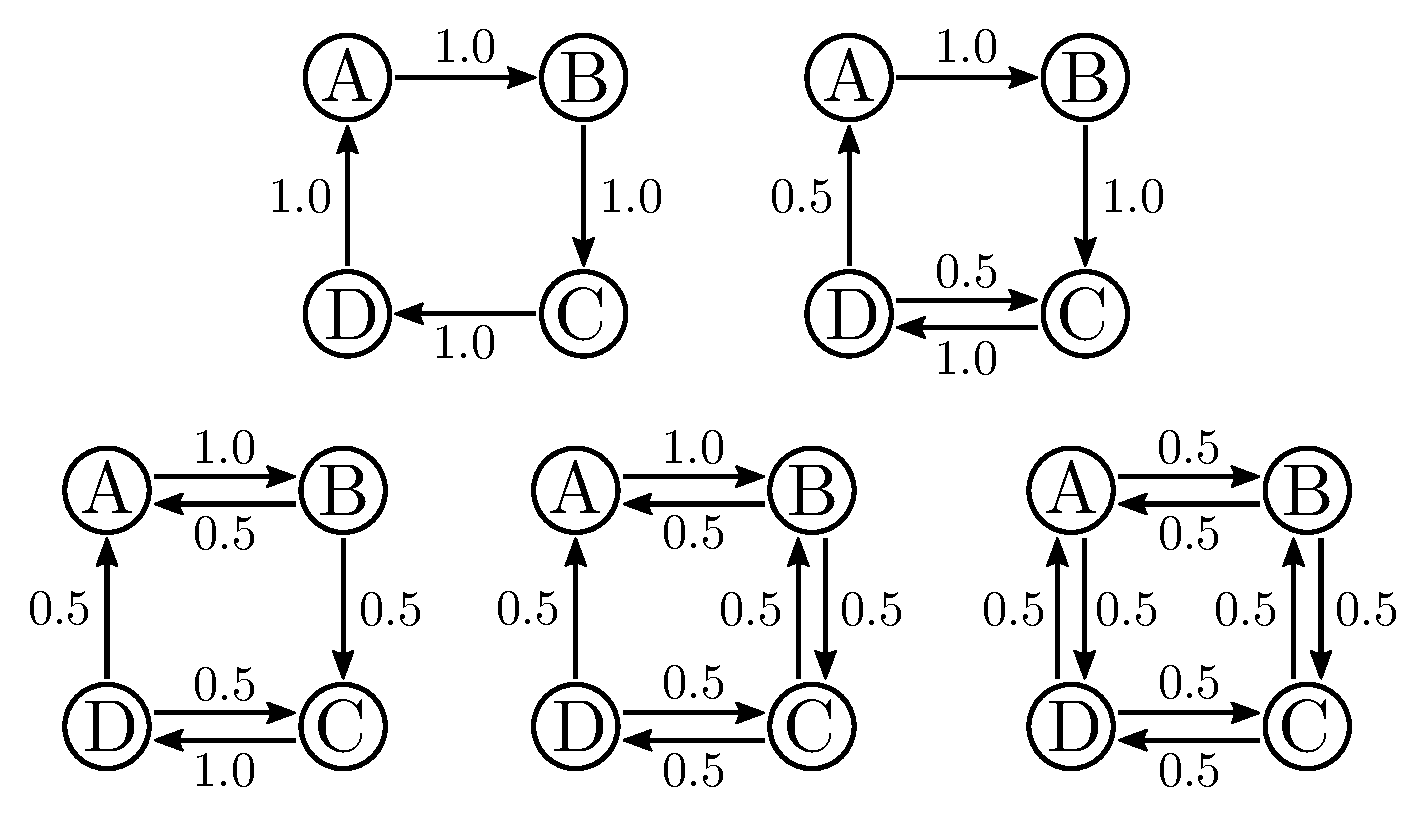
\includegraphics[width=0.85\textwidth]{results/mc1_models}
	\caption[First Markov models]{The first $4$ state Markov models, denoted as model series I. Starting point is a periodic Markov chain, where from model to model one more state is split with a probability of $p_{ij} = 0.5$. The models are enumerated from left to right and from top to down from $1$ to $5$.}
	\label{fig:mc1-models}
\end{figure}

Since there are many combinations of possible Markov chains, in the beginning a discrete state space of size $n = 4$ is chosen with $S = \{A,B,C,D\}$. Furthermore $5$ different Markov chains --- called \emph{models} in the following --- were chosen, shown in figure \ref{fig:mc1-models}. The idea was to start from a periodic Markov chain and systematically introduce more and more backward flow with probability of $p_{ij} = 0.5$. It was hypothesized that:

\begin{itemize}
\item A periodic Markov chain should be learned easily.
\item The more states having probability backward, the harder it can be learned.
\end{itemize}

\paragraph{Performance}

\begin{table}[!b]
\centering
\begin{tabular}{c|ccccc}
Model & 2 & 3 & 4 & 5 \\
\hline
\multirow{2}{*}{1} & $1.303\cdot 10^{-20}$ & $1.803\cdot 10^{-19}$ & $4.656\cdot 10^{-13}$ & $\mathbf{0.986}$ \\
 & ($18.51$) & ($17.14$) & ($10.73$) & ($0.02$) \\
\hline
\multirow{2}{*}{2} & & $1.561\cdot 10^{-05}$ & $1.099\cdot 10^{-15}$ & $8.475\cdot 10^{-21}$ \\
& & ($4.95$) & ($13.12$) & ($18.75$) \\
\hline
\multirow{2}{*}{3} & & & $6.310\cdot 10^{-12}$ & $8.091\cdot 10^{-20}$ \\
& & & ($9.78$) & ($17.55$) \\
\hline
\multirow{2}{*}{4} & & & & $6.284\cdot 10^{-14}$ \\
& & & & ($11.49$) \\
%\hline
\end{tabular}
\vspace{5pt}
\caption[p-values of performance differences between Markov models]{$p$-values of transition performance differences between Markov models. The upper value is the $p$-value, the lower value in brackets is the $T$ value. Obviously all values are highly significant, except the bold value which represents the $p$-value of the performance difference between model $1$ and $5$.}
\label{tb:mc1-t-test}
\end{table}

\begin{figure}[p]
    \centering
    \begin{subfigure}{0.48\textwidth}
    	\centering
        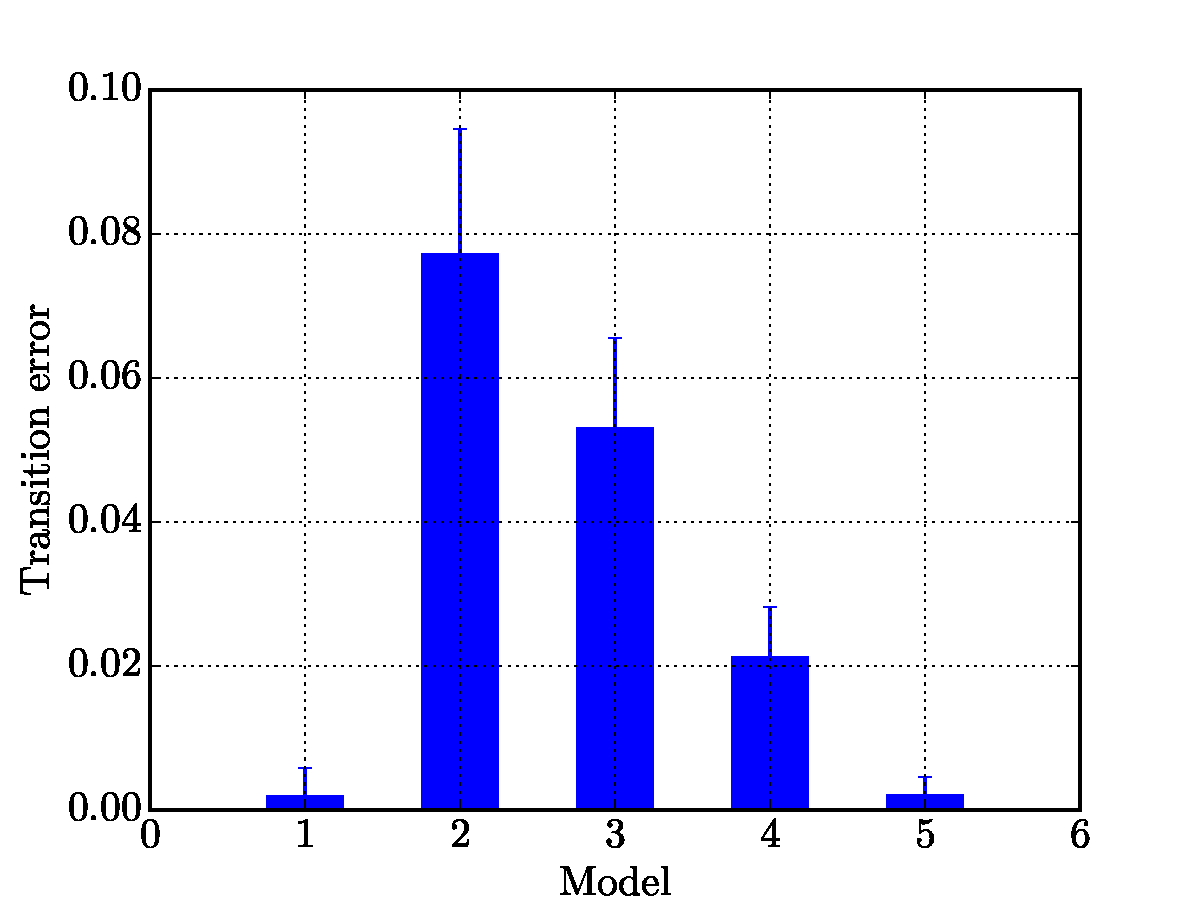
\includegraphics[width=\textwidth]{results/mc1_performance_distances}
        \caption{}
        \label{fig:mc1-performance-transition}
    \end{subfigure}
    \hfill
    \begin{subfigure}{0.48\textwidth}
    	\centering
        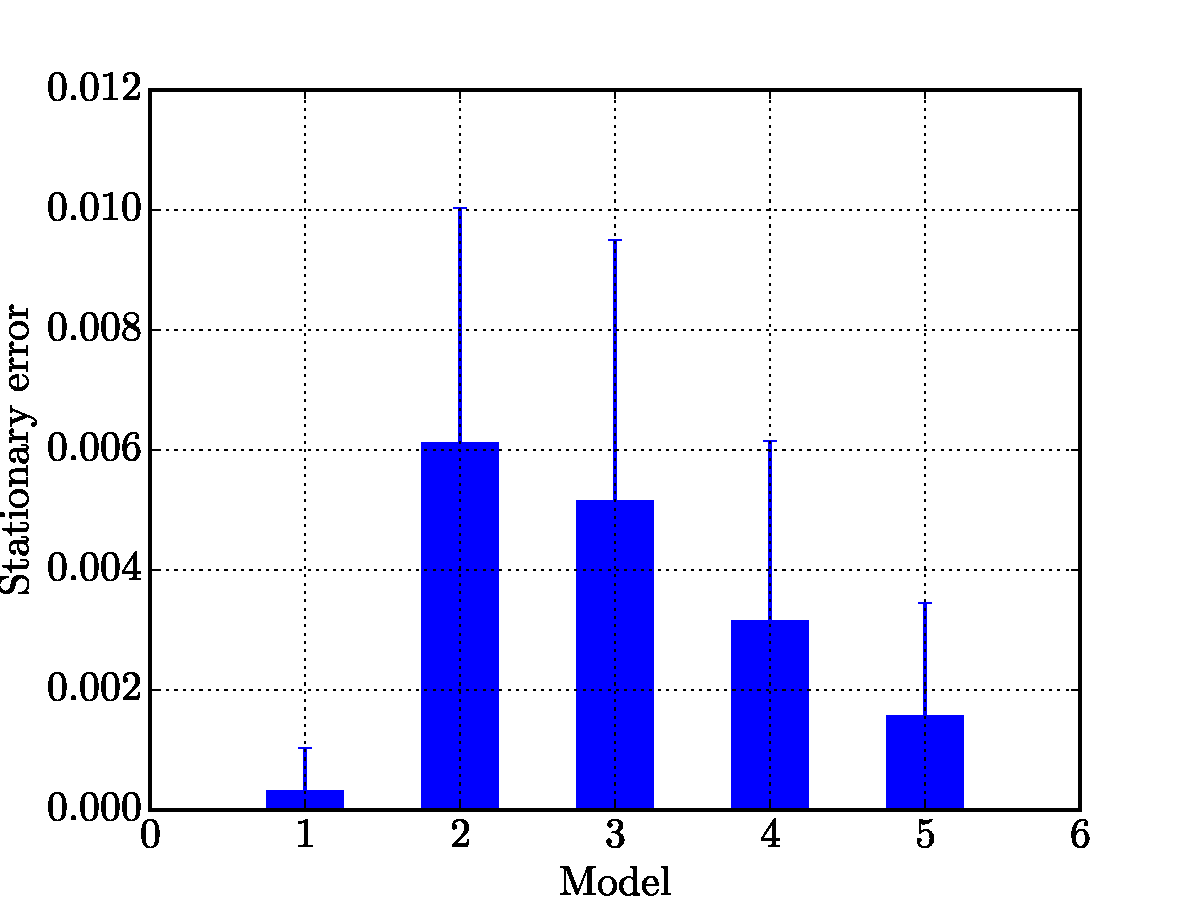
\includegraphics[width=\textwidth]{results/mc1_performance_stationary}
        \caption{}
        \label{fig:mc1-performance-stationary}
    \end{subfigure}
    \begin{subfigure}{0.48\textwidth}
    	\centering
        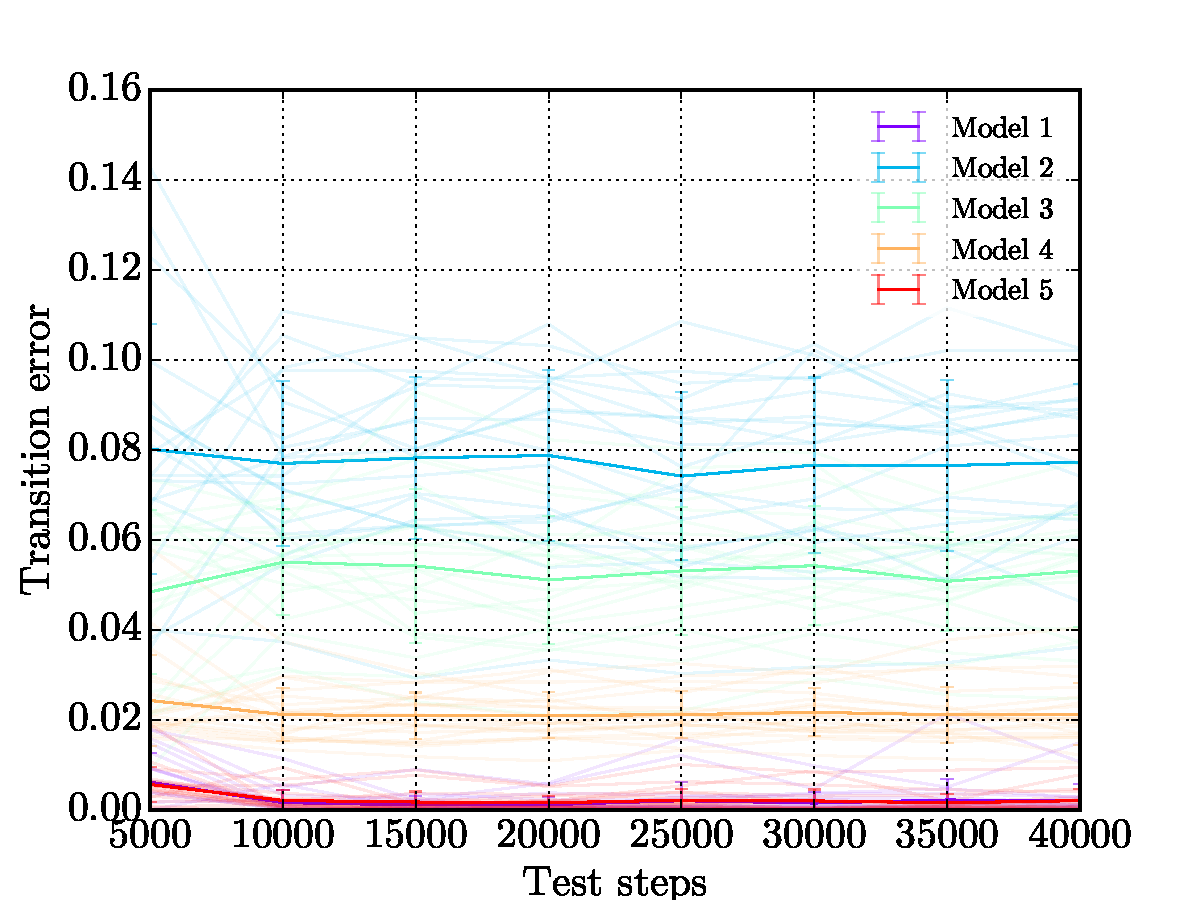
\includegraphics[width=\textwidth]{results/mc1_test_traces_distances}
        \caption{}
        \label{fig:mc1-test_traces-transition}
    \end{subfigure}
    \hfill
    \begin{subfigure}{0.48\textwidth}
    	\centering
        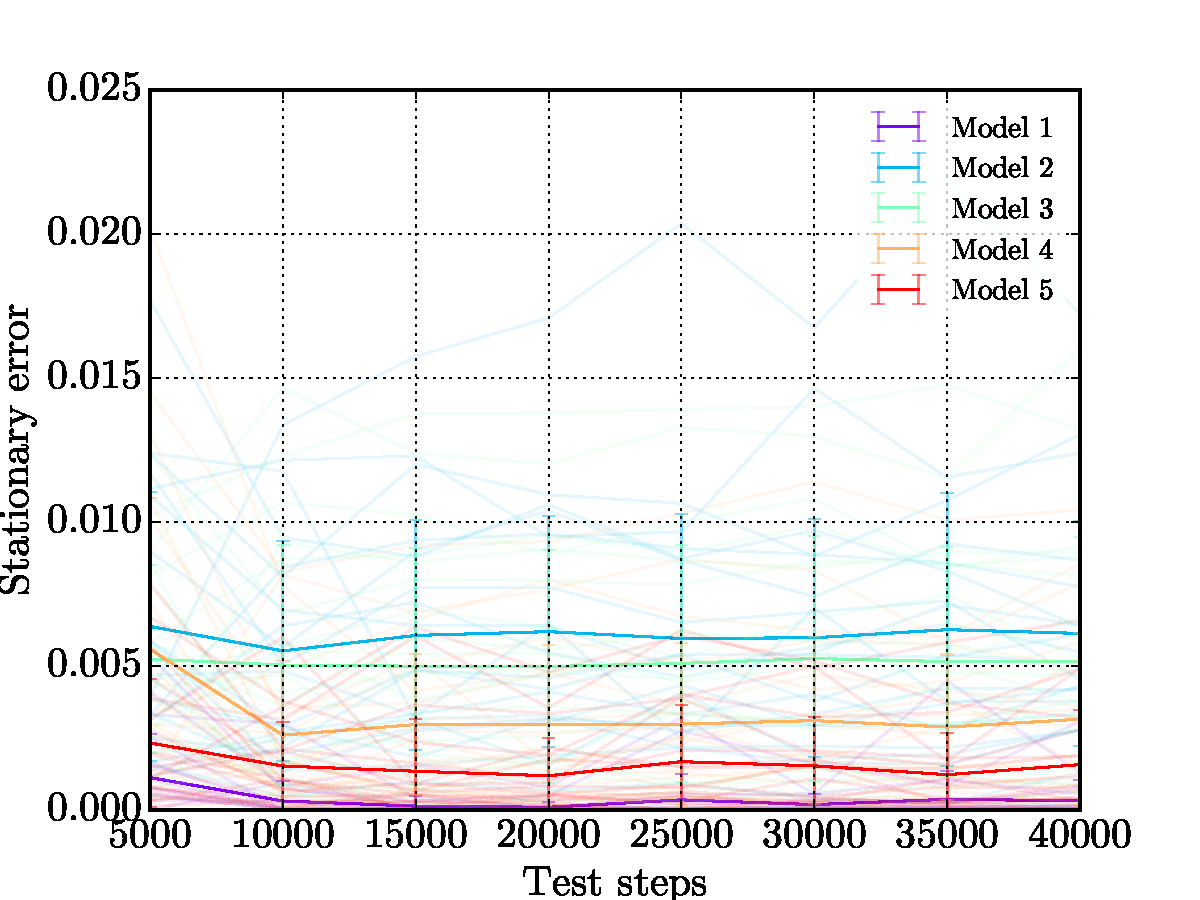
\includegraphics[width=\textwidth]{results/mc1_test_traces_stationary}
        \caption{}
        \label{fig:mc1-test_traces-stationary}
    \end{subfigure}
    \caption[Performance of first Markov models]{Performance of first Markov models. The transition error $\varepsilon_M$ of the first and last model is very low, as can be seen in in \textbf{a)}. The same holds for the stationary error $\varepsilon_\pi$ in \textbf{b)}. The error bars in \textbf{a)} and \textbf{b)} indicate standard errors. The $\varepsilon_M$ and $\varepsilon_\pi$ correspond to the last chunk in the testing phase. The error over all chunks in the testing phase is shown in \textbf{c)} and \textbf{d)}.}
    \label{fig:mc1-performance}
\end{figure}

In figures \ref{fig:mc1-performance-transition} and \ref{fig:mc1-performance-stationary} the performance of the $5$ models is shown. While the first hypothesis is true, the periodic Markov chain can be learned with high performance, the second hypothesis is not true. There is no relation between the number of backward directions and the performance. Furthermore, the performance differences between the models seem high. Results of t-tests show that all models differ highly significant with $p < 0.0001$ in transition performance $\varepsilon_M$, except between model $1$ and $5$ where $p=0.986$, where the null hypothesis cannot be rejected. Table \ref{tb:mc1-t-test} shows the results of all t-test pairs. An example for a learned transition matrix is shown in table \ref{tb:mc1-example}.

Additionally the performance over time was plotted in figures \ref{fig:mc1-test_traces-transition} and \ref{fig:mc1-test_traces-stationary}, showing that the performance is stable over time in testing phase. This is reasonable, since \acl{stdp} is not active in testing phase and the weights stay constant. To prove that \acs{stdp} is the cause for the stable behavior, another simulation was done in appendix \ref{sec:appendix:stdp}, where \acs{stdp} was switched on in the testing phase. And indeed, the information is lost by time and the network `forgets' if \acs{stdp} is active and the weights are still plastic. Furthermore, after the first testing chunk from $5,000$ to $10,000$ steps, there is a slight drop in error. This is due to a burn in phase, which depends on $\eta_\IP$. It takes some time until the spontaneous activity reaches a stable state. Details regarding the burn in phase are given in appendix \ref{sec:appendix:eta}.

\begin{table}[!b]
\centering
\begin{tabular}{ccccc}
\multicolumn{5}{c}{Initial transition} \\
\hline
& $A$ & $B$ & $C$ & $D$\\
$A$ & $0$ & $1.0$ & $0$ & $0$ \\
$B$ & $0.5$ & $0$ & $0.5$ & $0$ \\
$C$ & $0$ & $0.5$ & $0$ & $0.5$ \\
$D$ & $0.5$ & $0$ & $0.5$ & $0$
\end{tabular}
\qquad
\begin{tabular}{ccccc}
\multicolumn{5}{c}{Learned transition} \\
\hline
& $A$ & $B$ & $C$ & $D$\\
$A$ & $0.02$ & $\mathbf{0.75}$ & $0.02$ & $0.21$ \\
$B$ & $\mathbf{0.48}$ & $0.04$ & $\mathbf{0.47}$ & $0.01$ \\
$C$ & $0.02$ & $\mathbf{0.61}$ & $0.03$ & $\mathbf{0.34}$ \\
$D$ & $\mathbf{0.46}$ & $0.05$ & $\mathbf{0.48}$ & $0.01$
\end{tabular}
\vspace{5pt}
\caption[Example for a learned transition matrix]{Example for a learned transition matrix. On the left side, model $4$ is shown. The transition probabilities were used to train the network. On the right side, the learned transition matrix of model $4$ is shown. The probabilities are calculated using equation \eqref{eq:transition-estimation}. Bold values were initially non-zero. While most transitions are represented quite well by the network, the transition from $A$ to $B$ differs a lot.}
\label{tb:mc1-example}
\end{table}

In conclusion, the main interesting effect is that the models seem to perform differently and there is currently no explanation why they behave in that way. It is striking, that model $1$ and $5$ seem very simple. Model $1$ represents just a deterministic input pattern and \textcite{hartmann2015s} already showed that such an input is represented quite well in the network. On the other hand, model $5$ has kind of a `random' structure. Except connections between $A$ \& $C$ and $B$ \& $D$, everything else has no strong restrictions, whereas the other models have more restrictions. For example model $4$: If the network reaches state $A$, it can only change to state $B$, which is a strong restriction, since all the other transitions are allowed to change to two directions. The results, shown in table \ref{tb:mc1-example}, seem to support this explanation. It seems to be problematic to learn the connection between $A$ and $B$, a lot of probability is `lost' in this row.

The mean squared error from the transition matrix seems to be a sufficient measure. It is able to reflect the performance of the network and captures more information than the stationary distribution. Hence, in the following, only the performance measures obtained from the transition matrices  $\varepsilon_M$ are shown.

\paragraph{Plastic training}

\begin{figure}[!b]
	\centering
	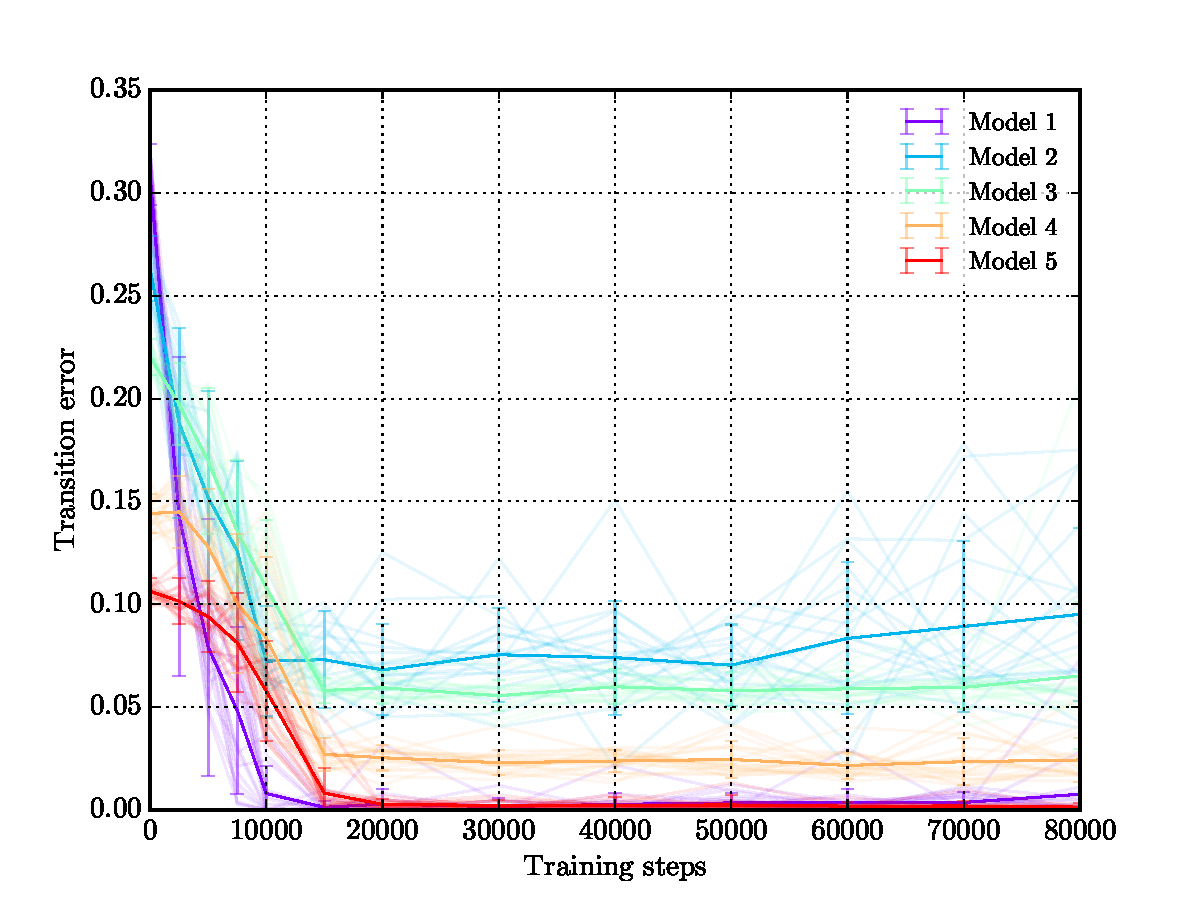
\includegraphics[width=0.95\textwidth]{results/mc1_distances_training_steps_transition}
	\caption[Influence of training to first Markov models]{Influence of training to first Markov models. The transparent lines are all $\Nsim=20$ simulations per model. The opaque lines represent the error $\varepsilon_M$ of a model per line for all simulations. Error bars indicate the standard error. Up to $T_\plastic = 20,000$ the steps were increased by $5,000$, after that, they were increased in steps of $10,000$. Model $1$ and $5$ saturate earlier than the other models, but finally all models reach a specific performance level and do not approximate each other. Training is not able to explain the performance differences between the models.}
	\label{fig:mc1-training}
\end{figure}

It is very likely that the network performs better if the time for training is increased. If absolutely no plastic training is applied, meaning that $T_\plastic = 0$, the network can be seen as a reservoir network. The weights are initialized, but not adapted to the input in that case. The more steps $T_\plastic$ are chosen, the better the performance should be, due to the \acs{stdp} mechanism. It could be that the $T_\plastic = 50,000$ training steps are not enough for all models. Perhaps, model $2$, $3$ and $4$ need a longer training to perform well. In order to understand the influence of the parameter, $T_\plastic$ was varied from $T_\plastic = 0$ to $T_\plastic = 80,000$. There are three hypothesis regarding the plastic training phase:

\begin{itemize}
\item All models improve in performance when training is extended and the performance increase is decreasing, the longer the training is conducted.
\item Different models need different self-organizing time for a good performance.
\item The longer the training period is, the closer the models get, regarding their performance.
\end{itemize}

The results in figure \ref{fig:mc1-training} show that the self-organizing phase has an important influence. The first hypothesis is partly true, since the performance increases, when more training is performed. But the increase in performance is saturating after about $T_\plastic \approx 20,000$ steps of plastic training.

Model $1$ and $5$ seem to saturate earlier (at about $T_\plastic \approx 10,000$) than the other models (at about $T_\plastic \approx 15,000$ to $T_\plastic \approx 20,000$). This behavior is in line with the second hypothesis. But since all of them are saturating, it contradicts the third hypothesis. At which point the network saturates, seems to depend slightly on the model, but still the previous differences remain after all. Differences in the length of the plastic training phase are not able to explain performance differences between models.

\paragraph{Size of the network and size of input cluster}

It is necessary to develop further ideas why the models have different performance in the same network. Another idea is to check the size of the network. It could be that --- for some reason --- some models need more neurons to find a good representation. It is important to also control the number of input connections to the network. If the network size is increased, but the number of connections between input neurons and excitatory neurons stays constant, it could be that the input information has too little influence, compared to ongoing spontaneous activity. In case of small input clusters, most of the network would just end up in spontaneous activity. Therefore, both parameters were varied at the same time. The network size was tested between $N^E = 100$ and $N^E = 500$ in steps of $\Delta N^E = 50$ and the number of input connections varied from $N^U_{x_i} = f_U \cdot N^E = 0.03 \cdot N^E$ to $N^U_{x_i} = 0.15 \cdot N^E$ in steps of $\Delta N^U_{x_i} = 0.01 \cdot N^E$. Since the number of inhibitory neurons depends on the number of excitatory neurons by $N^I = 0.2 \cdot N^E$, also the number of inhibitory neurons are changed.

\begin{figure}[p]
    \centering
    \begin{subfigure}{0.48\textwidth}
    	\centering
        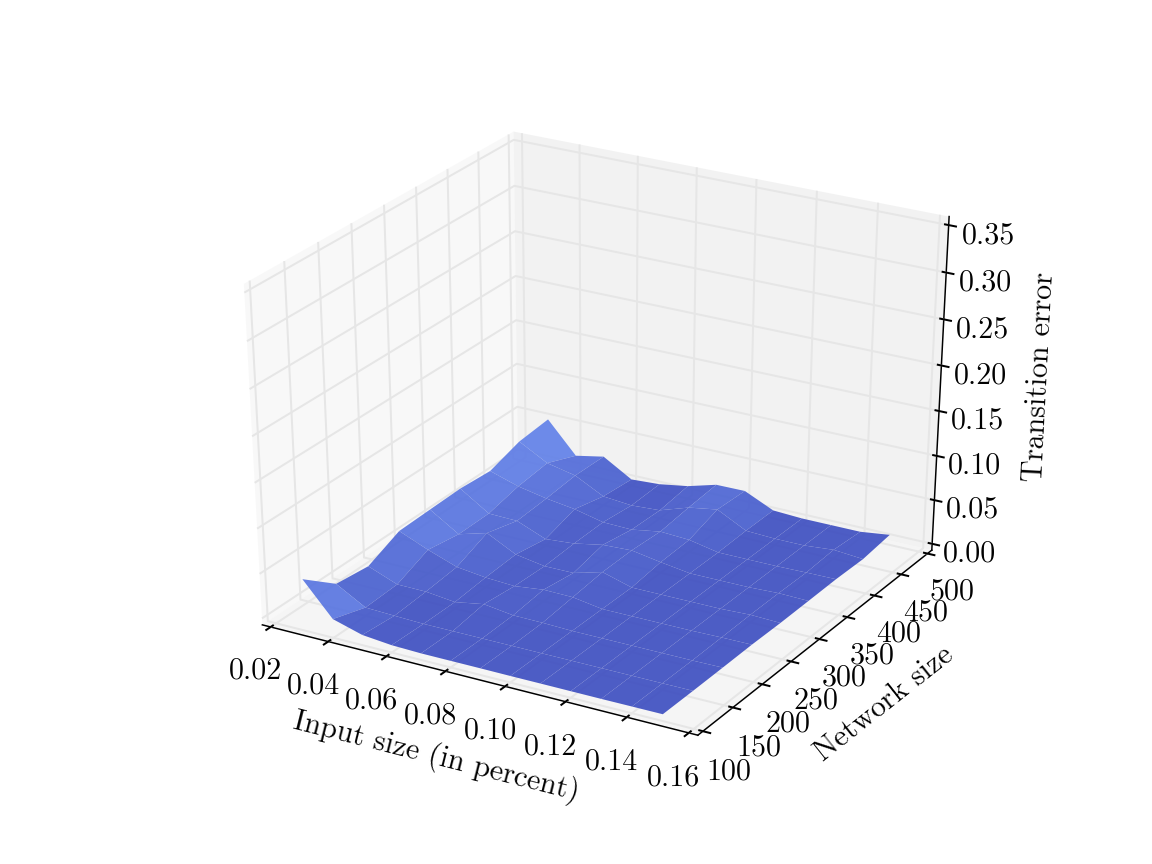
\includegraphics[width=\textwidth]{results/mc1_distances_size_inputs_0}
        \caption{Model $1$}
        \label{fig:mc1-size-0}
    \end{subfigure}
    \hfill
    \begin{subfigure}{0.48\textwidth}
    	\centering
        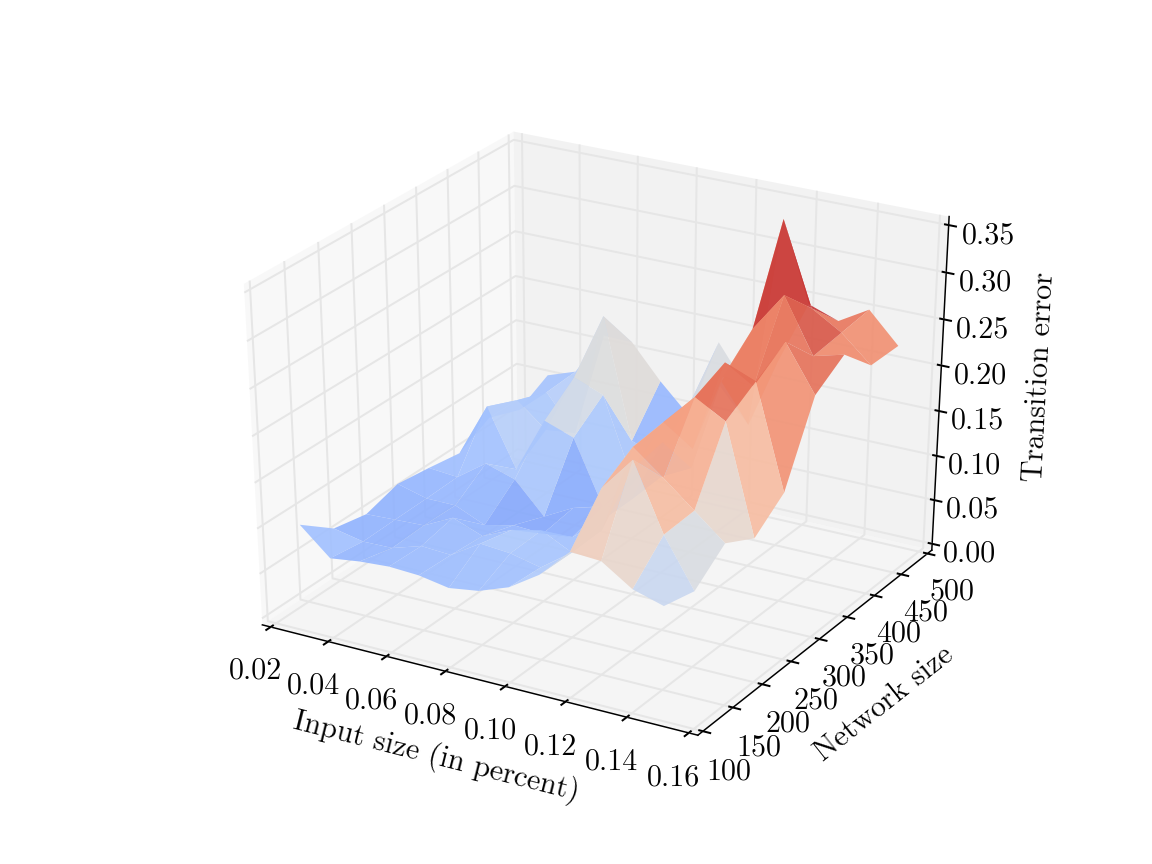
\includegraphics[width=\textwidth]{results/mc1_distances_size_inputs_1}
        \caption{Model $2$}
        \label{fig:mc1-size-1}
    \end{subfigure}
    \begin{subfigure}{0.48\textwidth}
    	\centering
        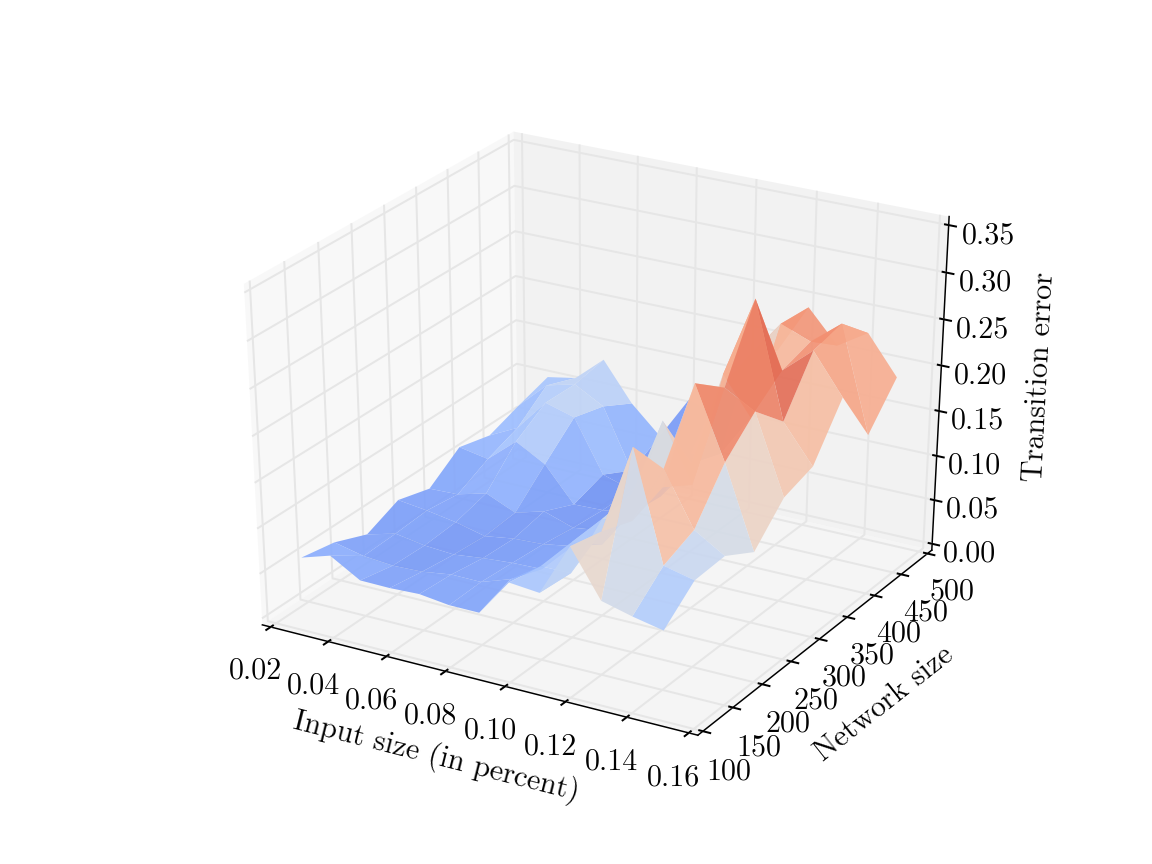
\includegraphics[width=\textwidth]{results/mc1_distances_size_inputs_2}
        \caption{Model $3$}
        \label{fig:mc1-size-2}
    \end{subfigure}
    \hfill
    \begin{subfigure}{0.48\textwidth}
    	\centering
        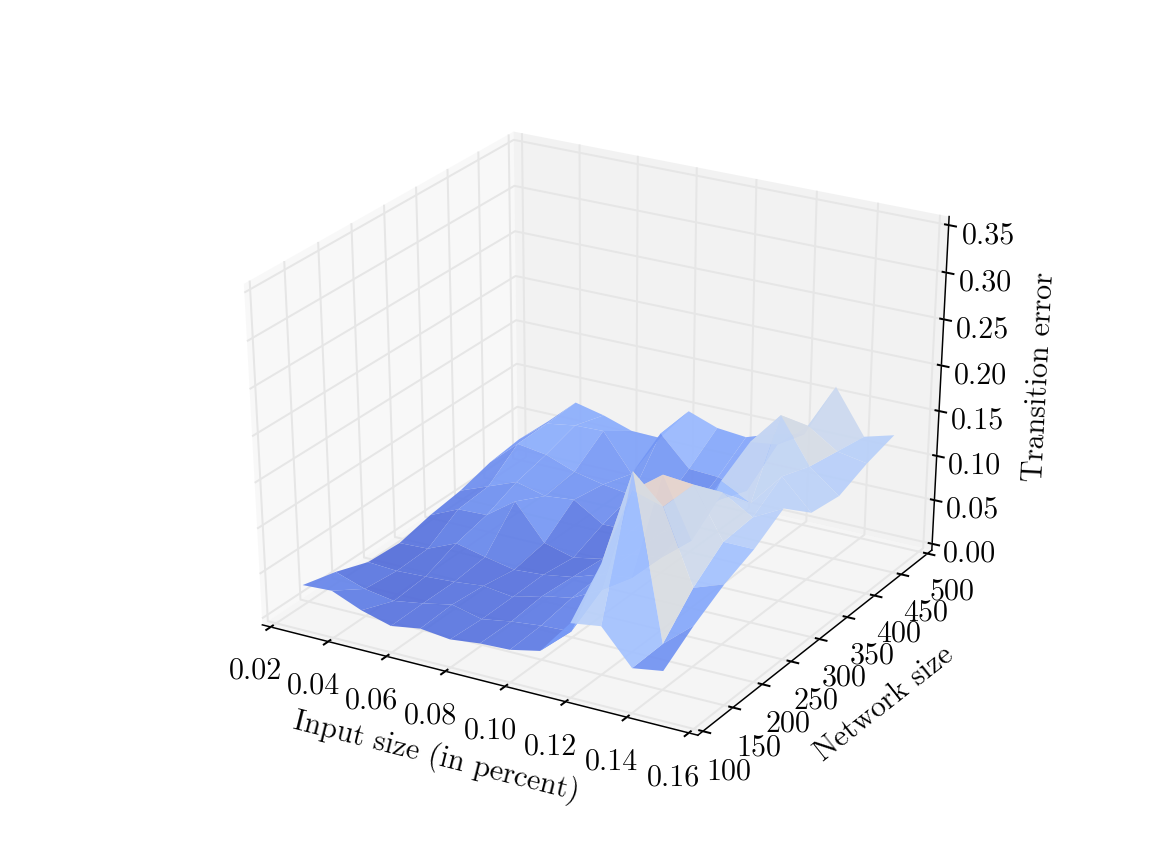
\includegraphics[width=\textwidth]{results/mc1_distances_size_inputs_3}
        \caption{Model $4$}
        \label{fig:mc1-size-3}
    \end{subfigure}
    \begin{subfigure}{0.48\textwidth}
    	\centering
        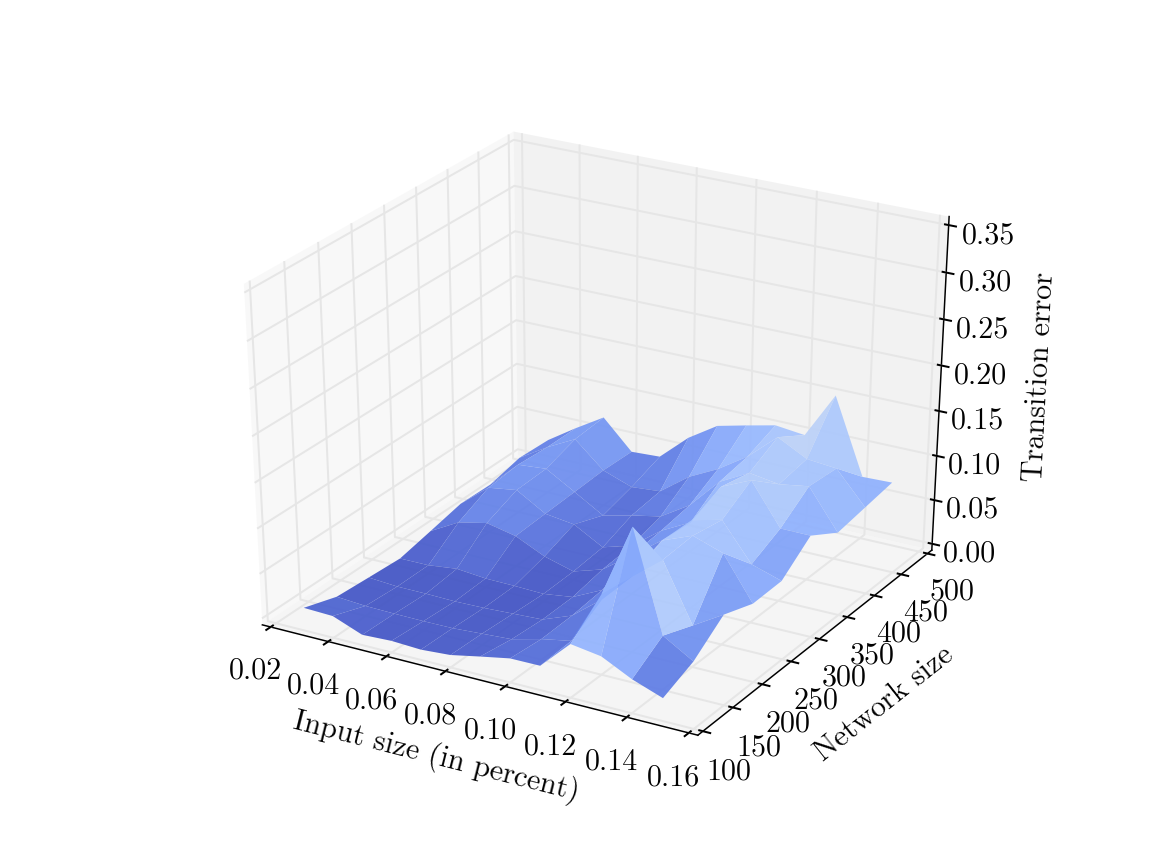
\includegraphics[width=\textwidth]{results/mc1_distances_size_inputs_4}
        \caption{Model $5$}
        \label{fig:mc1-size-4}
    \end{subfigure}
    \hfill
    \caption[Size of the network and size of the input cluster]{Shown is the performance of the $5$ models, depending on the number of excitatory neurons $N^E$ and the size of the input cluster   for every input $N^U_{x_i}$. $N^E$ was chosen from $100$ to $500$ in steps of $\Delta N^E = 50$. The size of the input cluster or equivalently the number of input-to-excitatory weights per input was chosen as a percentage of $N^E$ for every state. It is defined as $N^U_{x_i} = f_U \cdot N^E$, where $f_U$ was chosen between $0.03$ and $0.15$ in steps of $\Delta f_U = 0.01$. The two parameters do not explain the differences between the models.}
    \label{fig:mc1-size}
\end{figure}

In figure \ref{fig:mc1-size} the results are shown. Both parameters have an influence on the performance, but the mean performance is still different for the models. The initial parameters, proposed by \textcite{hartmann2015s}, of $N^E = 200$, $N^U = 0.2 \cdot 200 = 40$ and $N^U_{x_i} = 0.05 \cdot 200 = 10$ seem to have a good performance, compared to the other combinations. There are interesting effects worth to research on. There is a decay in performance for bigger networks, independent of the number of input connections. Furthermore, the performance decreases for more input connections, but the performance becomes better again for $f_U \ge 0.14$. But since the thesis focuses on the performance discrepancies between the different models, no further investigation was done. The main result is that the differences between the models could not be explained by the network size, nor by the size of the input clusters. While the optimal parameter combination is very similar for all models, the models still differ in their scales.

\paragraph{Classification method}

In section \ref{sec:state-classification}, the classification method was introduced. It was already mentioned that the original selection mechanism from \textcite{hartmann2015s}, to find the activity pattern representations $R_\compare$, was changed. The original method was taking the last $\tilde{T}_\compare = 2500$ steps of the no-plastic training phase. While working with the network, a bias in the classification method was found. The number of available comparison steps $T_\compare^\mini$ differed a lot between the models. Perhaps, the classification algorithm is connected to the differences in the performance. While the updated mechanism was already explained in the methods section theoretically, the original and the updated method will be applied to the case of the $5$ models in this section.

\begin{table}[!b]
\centering
\begin{tabular}{c|cccc}
Model & $\pi_A$ & $\pi_B$ & $\pi_C$ & $\pi_D$ \\
\hline
1 & $\frac{1}{4}$ & $\frac{1}{4}$ & $\frac{1}{4}$ & $\frac{1}{4}$ \\
2 & $\frac{1}{6}$ & $\frac{1}{6}$ & $\frac{2}{6}$ & $\frac{2}{6}$ \\
3 & $\frac{1}{4}$ & $\frac{1}{4}$ & $\frac{1}{4}$ & $\frac{1}{4}$ \\
4 & $\frac{2}{7}$ & $\frac{3}{7}$ & $\frac{2}{7}$ & $\frac{1}{7}$ \\
5 & $\frac{1}{4}$ & $\frac{1}{4}$ & $\frac{1}{4}$ & $\frac{1}{4}$
\end{tabular}
\vspace{5pt}
\caption[Stationary distributions of model series I]{Stationary distributions of first Markov models. In models $1$, $3$ and $5$ all states have equal probabilities, in models $2$ and $4$ the probabilities of the states differ.}
\label{tb:mc1-stat}
\end{table}

In models $1$, $3$ and $5$ every state is equally probable, which can be seen by the stationary distribution, provided in table \ref{tb:mc1-stat}. The stationary distributions for all $5$ models were calculated. The states $A$ and $B$ in model $2$ are less equal, than the others. The same holds for state $D$ in model $4$. In the no-plastic training phase, those states will occur less often, which is elaborated in the following. Note that for the calculation of the stationary distribution of model $1$, theorem \ref{th:markov-stat} cannot be applied, since the model is periodic. In that case only theorem \ref{th:irr-rec} can be applied and model $1$ has no limiting distribution.

In average it is expected that every state  occurs $\tilde{T}_\compare \cdot \pi_{x_i}$. If all states have the same probability, it results in $\tilde{T}_\compare / n = 2500 / 4 = 625$ steps for every state in the comparison phase. The calculation leads to $T_\compare^\mini = \min\{ \tilde{T}_\compare^A, \tilde{T}_\compare^B, \tilde{T}_\compare^C, \tilde{T}_\compare^D \} = \min\{ 625, 625, 625, 625 \} = 625$ states in average, which are available as representative states for the classification. This expected number of steps for every state holds for models $1$, $3$ and $5$. But, for example, for model $2$, the state with the lowest probability is state $A$ and $B$ with $\pi_A = \pi_B = 1/6$. Hence, both states are expected to occur in $2500 \cdot 1/6 \approx 417$ cases. In average the number of available steps for every state is given by $T_\compare^\mini = \min\{ 417, 417, 833, 833 \} = 417$. With an analogous calculation it can be shown that for model $4$ only $357$ steps are available to compare with. The number of available samples for classification is nearly half of the available samples, compared to the models where all states are equally probable.

\begin{figure}[!b]
    \centering
    \begin{subfigure}{0.48\textwidth}
    	\centering
        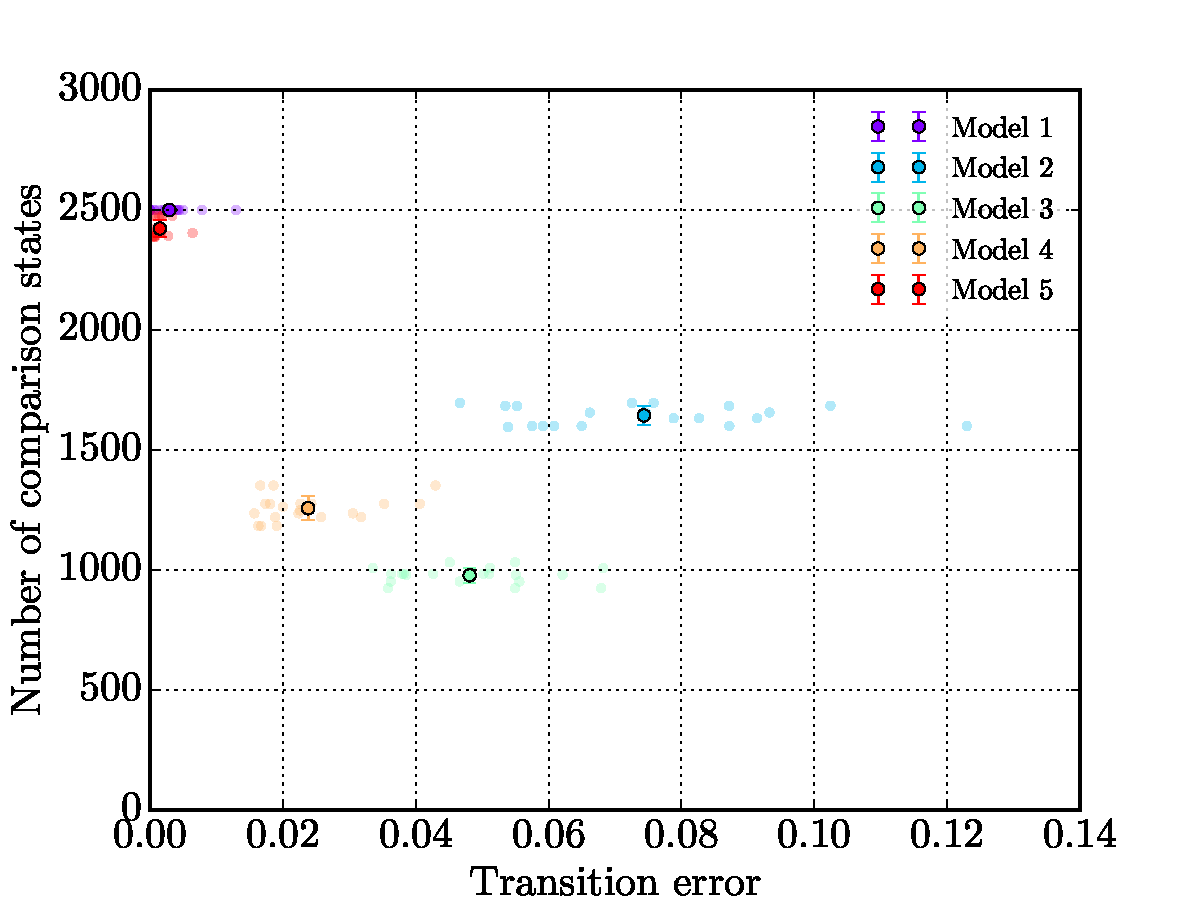
\includegraphics[width=\textwidth]{results/mc1_ncomparison_distances_old}
        \caption{Original method}
        \label{fig:mc1-comparison-old}
    \end{subfigure}
    \hfill
    \begin{subfigure}{0.48\textwidth}
    	\centering
        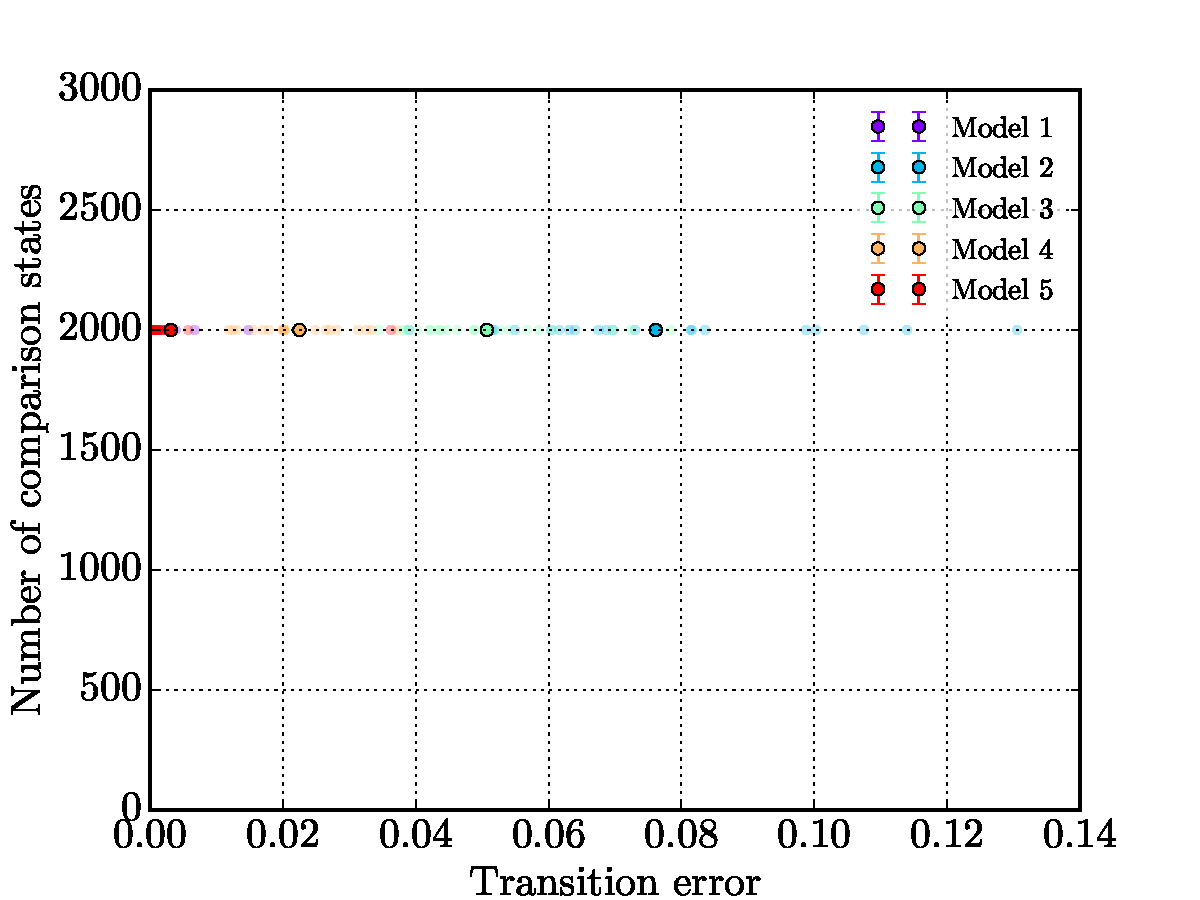
\includegraphics[width=\textwidth]{results/mc1_ncomparison_distances_new}
        \caption{Updated method}
        \label{fig:mc1-comparison-new}
    \end{subfigure}
    \caption[Available steps for comparison]{Available steps for comparison $n\cdot T_\compare^\mini$ with the original method and the updated method in relation to the performance. Transparent points are the single simulations, the opaque points represent their means. Error bars are added for the standard errors of $n\cdot T_\compare^\mini$, but they are very small. The evaluation of the original method is shown in \textbf{a)}. The performance of the transition error seems to depend negative on the transition error, in tendency. Figure \textbf{b)} shows the result if $n\cdot T_\compare$ is fixed. There is no effect by design.}
    \label{fig:mc1-comparison}
\end{figure}

It was hypothesized, that the original selection mechanism influences the performance systematically. There should be a correlation between $T_\compare^\mini$ and the performance $\varepsilon_M$ of the specific model. In figure \ref{fig:mc1-comparison-old} the overall number of available comparison steps $T_\compare^\mini \cdot n$ is shown at the $y$-axis. The error $\varepsilon_M$ is at the $x$-axis. The plot shows that there is indeed a slight negative effect. Of course, there is a ceiling effect since the highest possible $T_\compare^\mini$ is $625$, and therefore also $T_\compare^\mini \cdot n$ has a limit. Additionally, the effect seems not perfectly clear, but still, the correlation is $r_{T\compare} = -0.63$.

The updated mechanism fixes the number of $T_\compare = 500$. An algorithm was searching for the last $500$ representatives for every state in the no-plastic training phase, starting from the end. In that case, independent of the model, the same number of steps is available for classification. The number of necessary no-plastic training $\tilde{T}_\compare$ steps is flexible in that case, which influences the choice of $T_\noplastic$. In the old method the number of no-plastic training steps could easily be estimated, since they never exceeded $\tilde{T}_\compare = 2500$. In the new solution the overall number $\tilde{T}_\compare$ depends on the probability of that state which occurs least. An example was given in section \ref{sec:state-classification}.

The new classification method was also tested. The results with the updated method is shown in figure \ref{fig:mc1-comparison-new}. This time there is no correlation any more, which is expected, since the ceiling is always reached from every model by design. Lastly, the performance measures of all models were compared again with the new method. Surprisingly, even though the correlation is controlled, there is no clear change in the behavior. Hence, there has to be another mechanism responsible for the performance differences between the models. However, the idea to concentrate on the properties of the Markov chain, in terms of the stationary distribution, seemed to be an interesting approach to focus on.

\paragraph{Information of the stationary distribution}

\begin{figure}[!b]
	\centering
	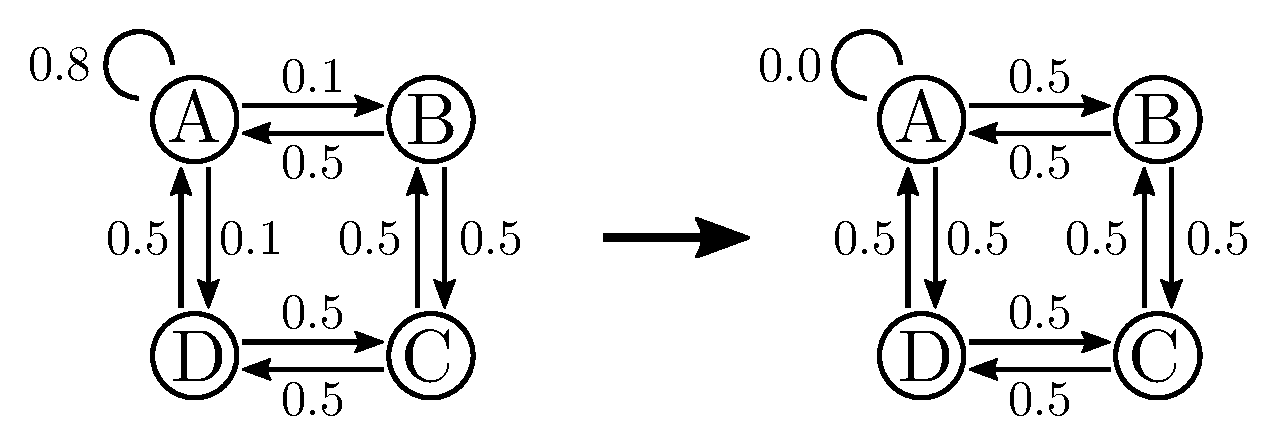
\includegraphics[width=0.85\textwidth]{results/mc2_models}
	\caption[Markov model series II]{Model series II. This time, it is very probable that state $A$ stays in state $A$, whereas $B$, $C$ and $D$ change between each other with equal probability (except $B$ and $D$). Starting from this model, in several steps the probability $p_{AA}$ is decreased to $p_{AA} = 0$ and $p_{AB}$ and $p_{AD}$ are increased to $p_{AB} = p_{AD} = 0.5$. The stationary distributions of all models are shown in table \ref{tb:mc2-stat}.}
	\label{fig:mc2-models}
\end{figure}

In the previous section, the stationary distribution was used to obtain the probabilities for every state. While the research was focused on the parameters of the network only, like the training or size, it would also be possible to focus on the statistical properties of the Markov chain in order to understand what kind of Markov chain can be learned better. In other words, it would be interesting to focus on the properties of the input instead of the network. Since the probabilities indirectly had an effect on the performance in the classification mechanism, it could also be that they directly have an influence. In the previous section, those Markov chains had an influence, where some states had a lower probability than others. This is finally due to a higher variance or due to a higher deviation from the perfectly equally stationary distribution. The latter could be measured by a Kullback-Leibler divergence between a perfectly equally distributed stationary and the present stationary distribution. Both measures were introduced in section \ref{sec:markov-measures}. It is hypothesized that Markov chains with different variance and Kullback-Leibler divergence vary in their performance systematically.

\begin{figure}[p]
    \centering
    \begin{subfigure}{0.48\textwidth}
    	\centering
        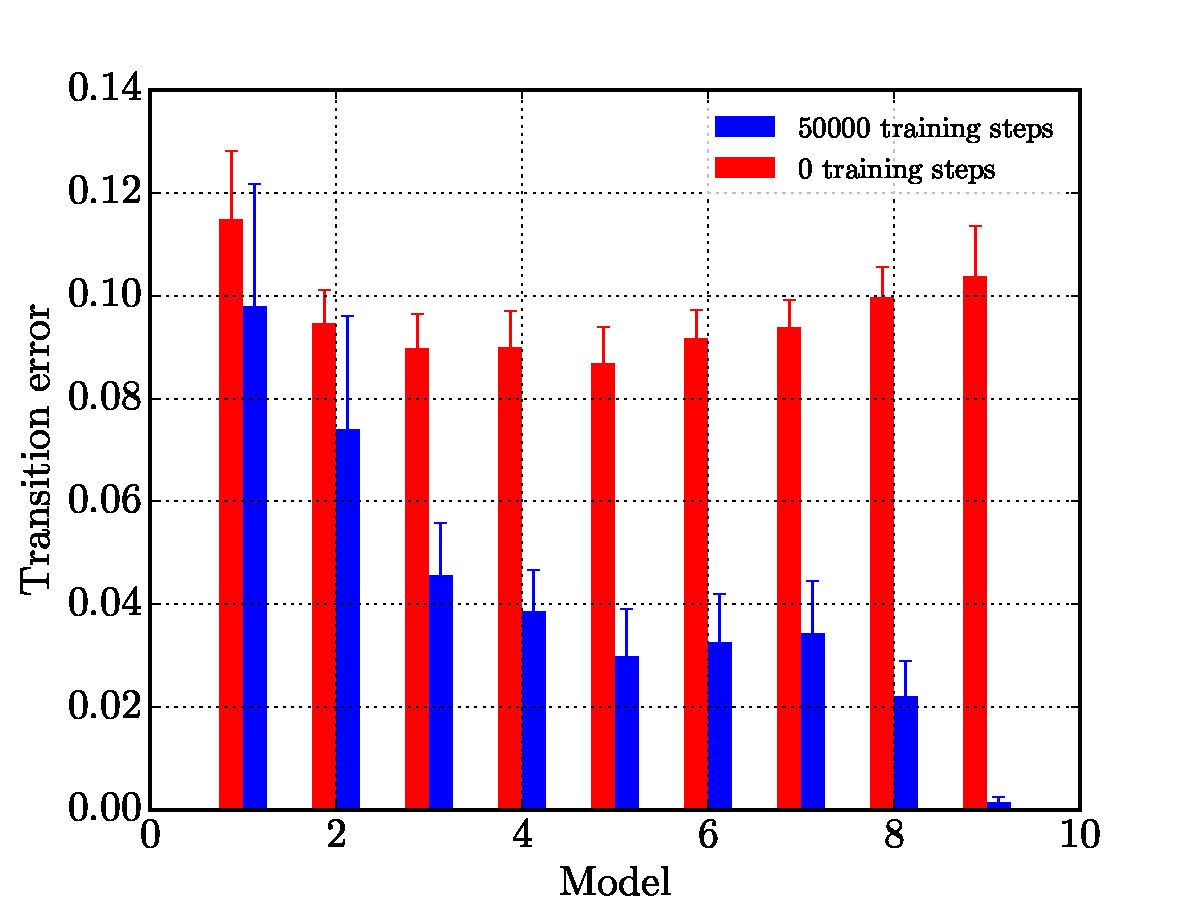
\includegraphics[width=\textwidth]{results/mc2_performance_distances}
        \caption{}
        \label{fig:mc2-performance-distance}
    \end{subfigure}
    \hfill
    \begin{subfigure}{0.48\textwidth}
    	\centering
        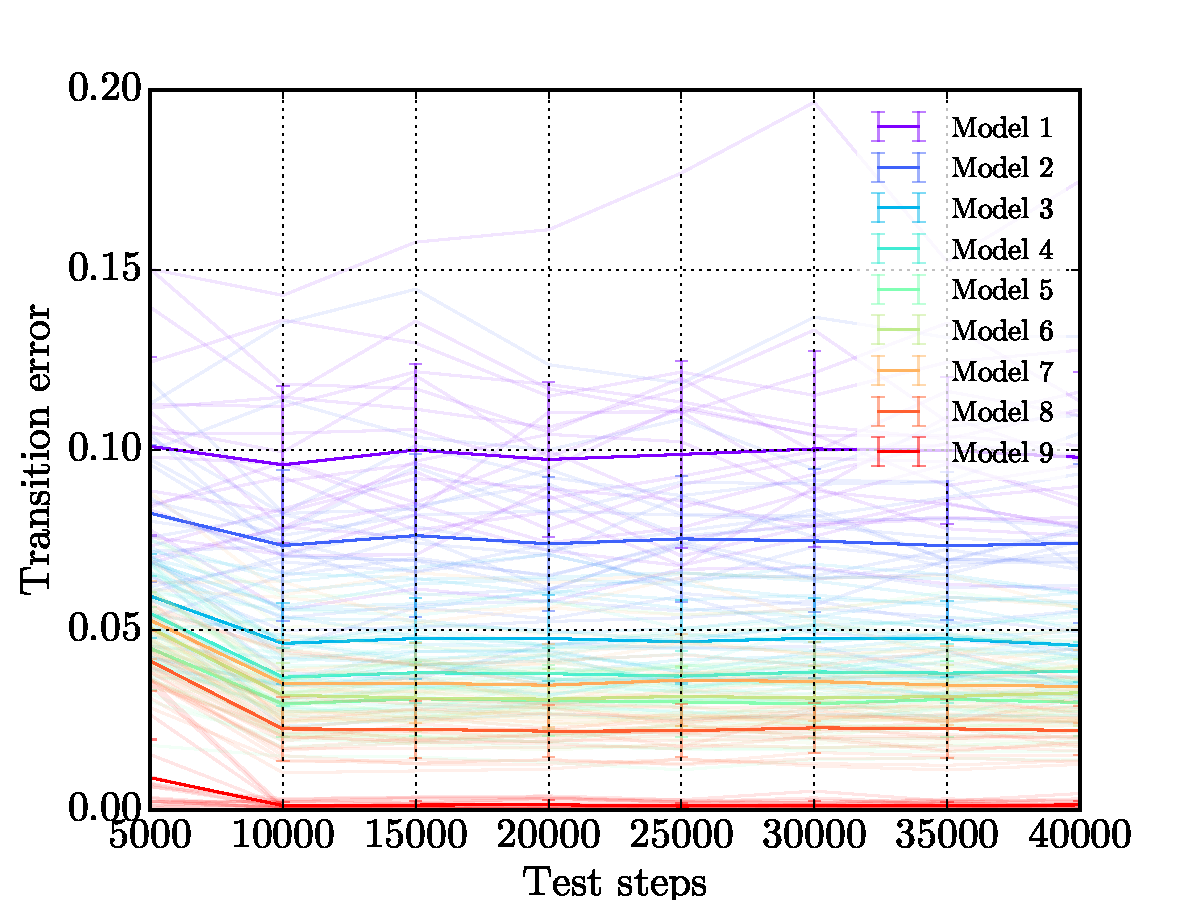
\includegraphics[width=\textwidth]{results/mc2_test_traces_distances}
        \caption{}
        \label{fig:mc2-trace-distance}
    \end{subfigure}
    \begin{subfigure}{0.48\textwidth}
    	\centering
        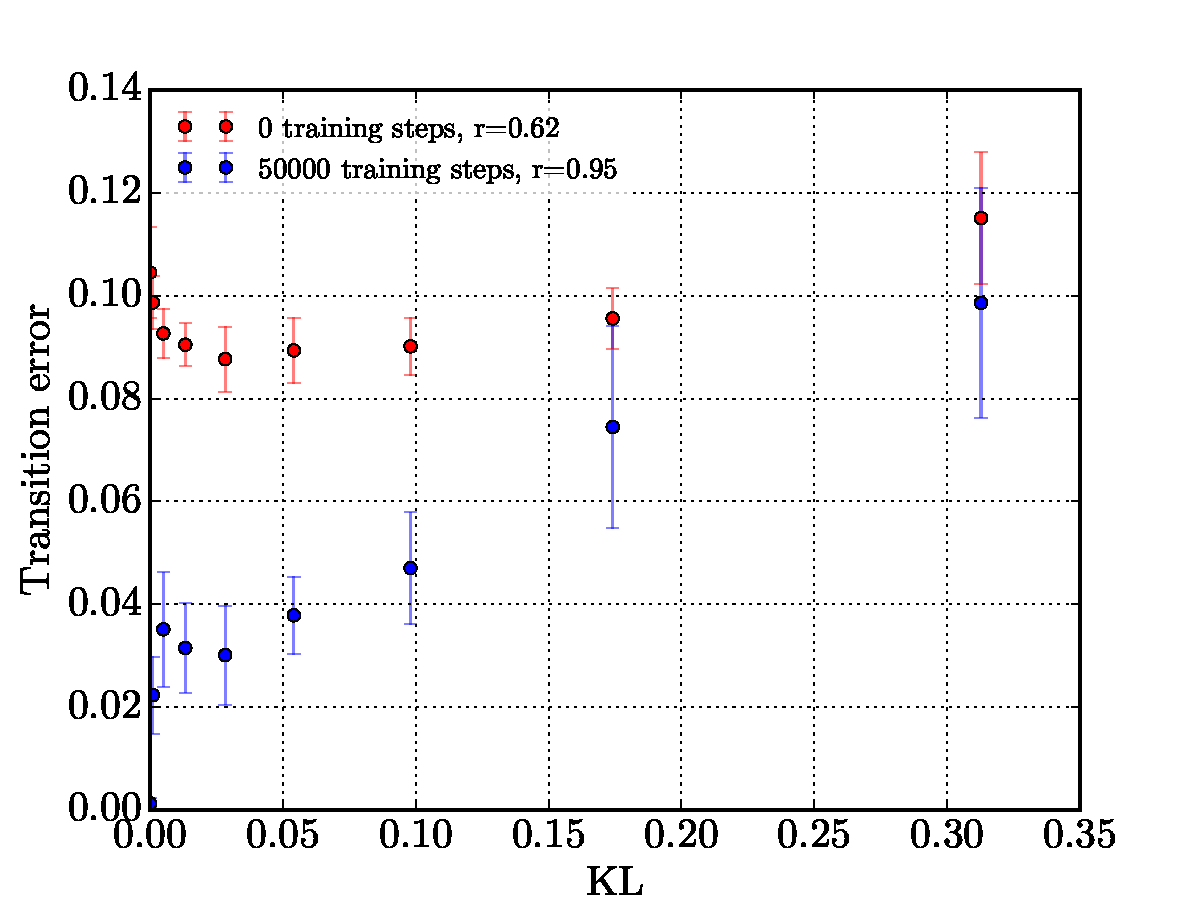
\includegraphics[width=\textwidth]{results/mc2_correlation_inequality_kl_train}
        \caption{}
        \label{fig:mc2-kl}
    \end{subfigure}
    \hfill
    \begin{subfigure}{0.48\textwidth}
    	\centering
        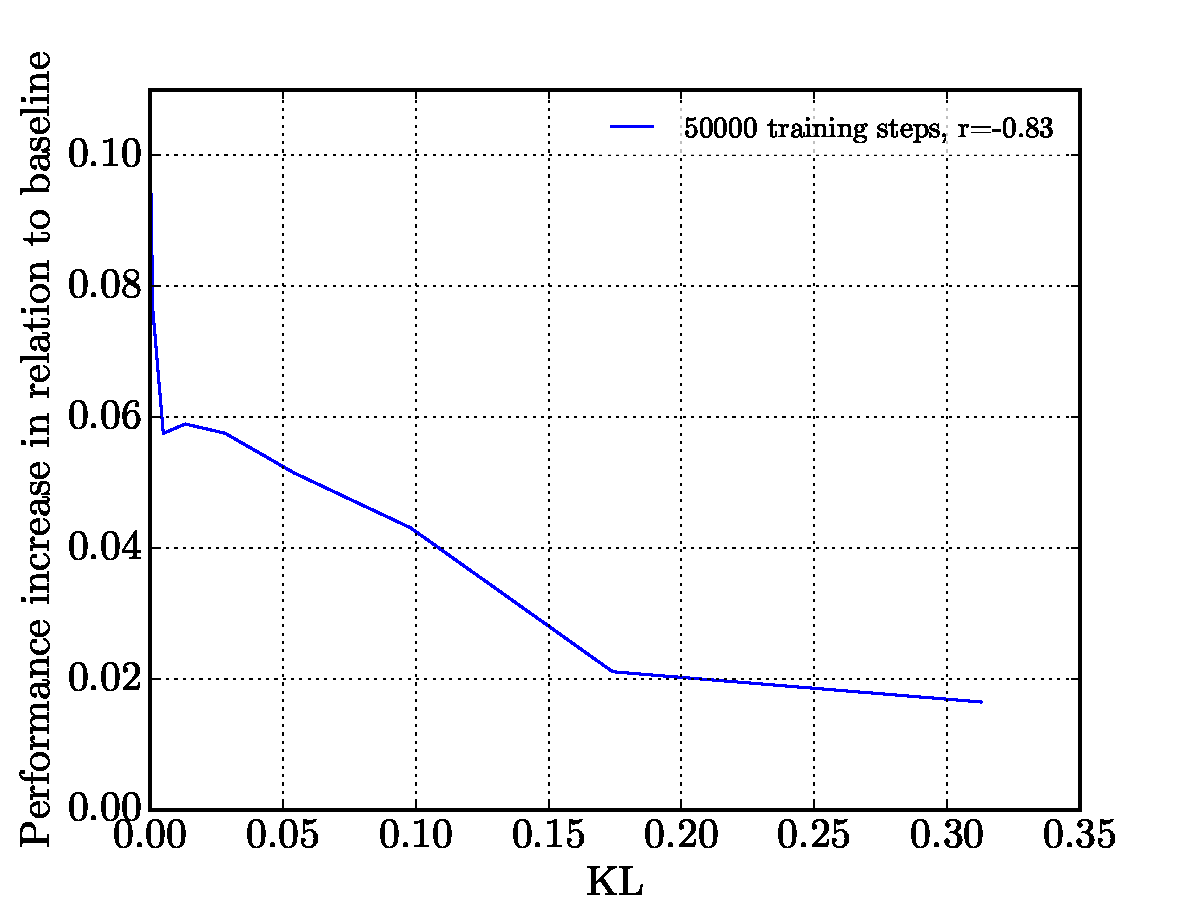
\includegraphics[width=\textwidth]{results/mc2_correlation_inequality_kl_train_baseline}
        \caption{}
        \label{fig:mc2-kl-baseline}
    \end{subfigure}
    \begin{subfigure}{0.48\textwidth}
    	\centering
        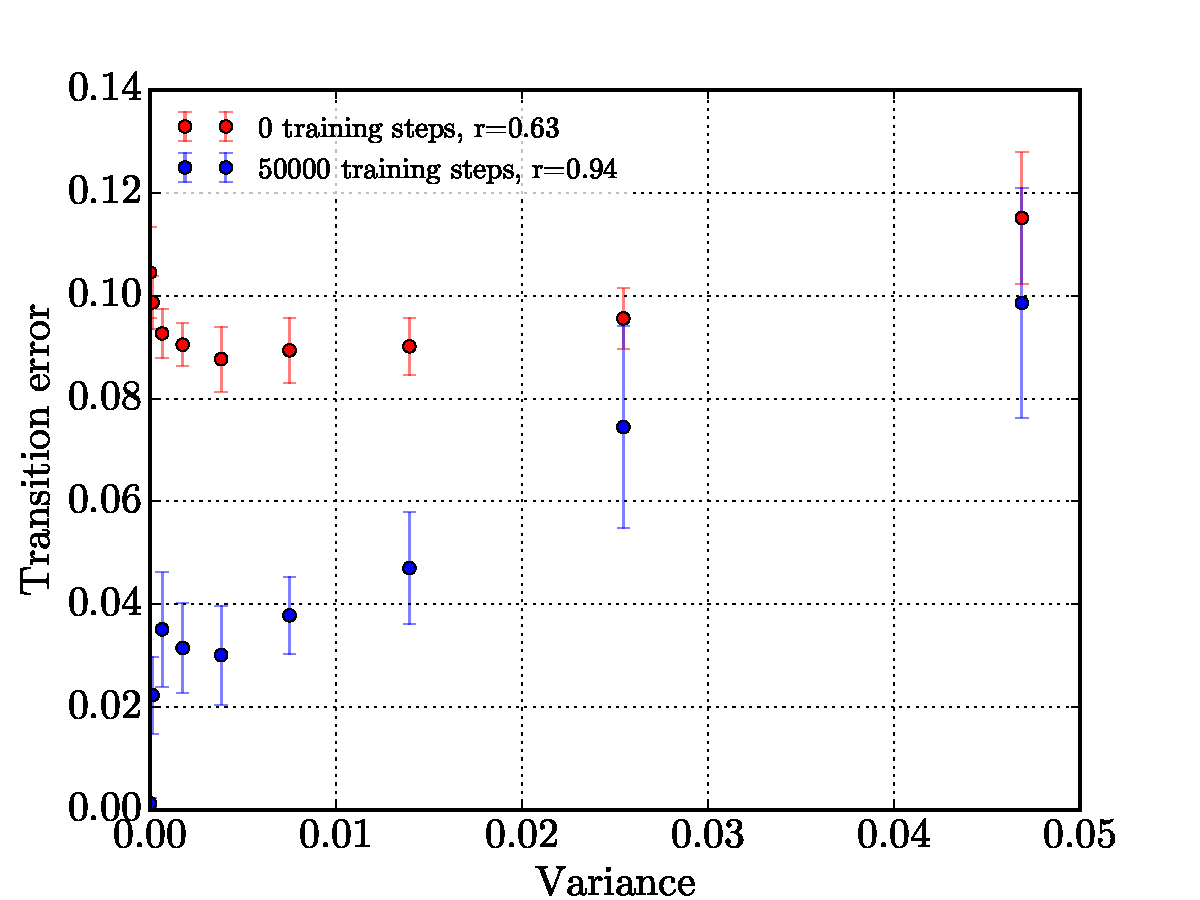
\includegraphics[width=\textwidth]{results/mc2_correlation_inequality_variance_train}
        \caption{}
        \label{fig:mc2-variance}
    \end{subfigure}
    \hfill
    \begin{subfigure}{0.48\textwidth}
    	\centering
        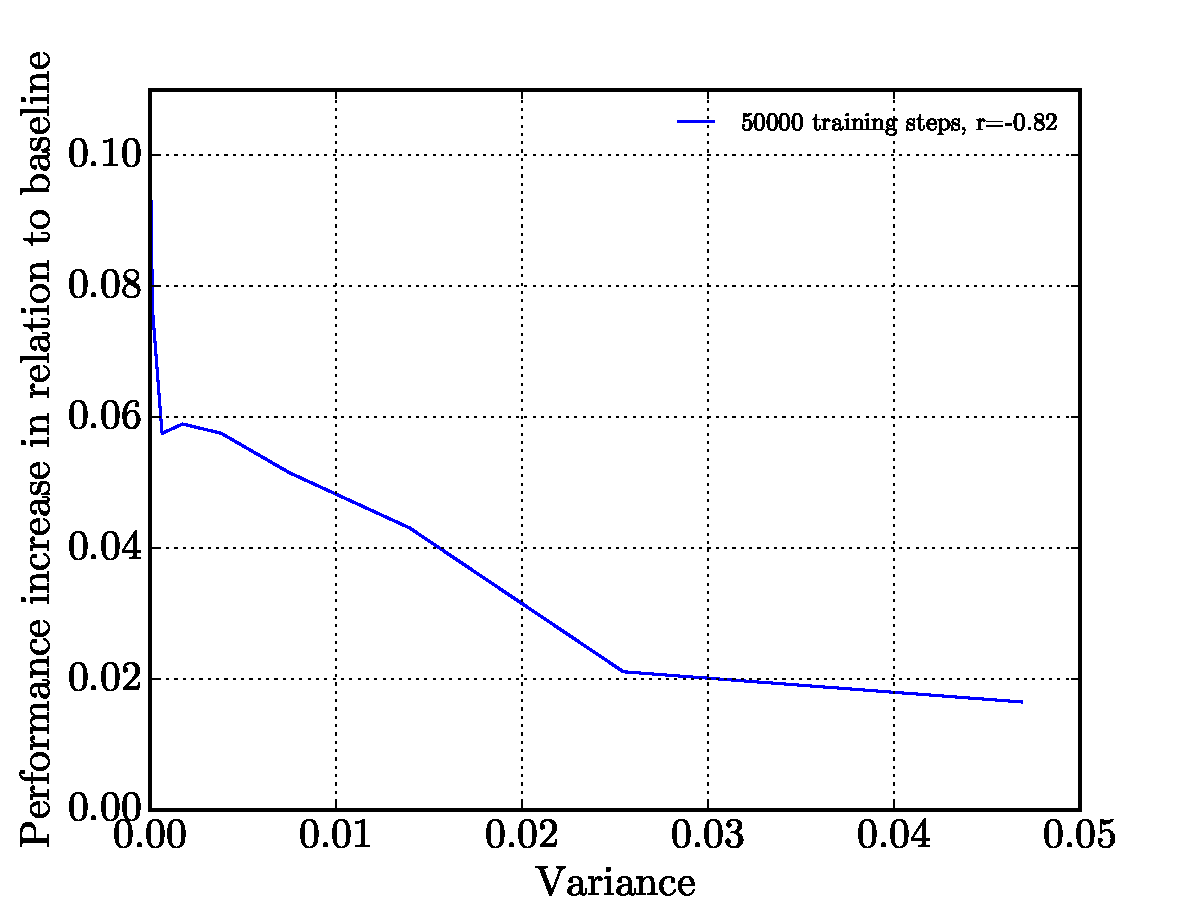
\includegraphics[width=\textwidth]{results/mc2_correlation_inequality_variance_train_baseline}
        \caption{}
        \label{fig:mc2-variance-baseline}
    \end{subfigure}
    \caption[Performance and information of model series II]{Performance and information of model series II. \textbf{a)} shows the performance of the $9$ models. Blue bars show the performance with $50,000$ plastic training steps, red bars with no training, which equals a static reservoir. The performance behavior over the testing phase for the trained network is shown in \textbf{b)} and is constant, as it was expected from previous results. Plot \textbf{c)} shows the correlation between the Kullback-Leibler divergence and the transition error $\varepsilon_M$. Correlations are given in the legend. In \textbf{d)} the increase in performance from the models with $50,000$ plastic training steps in relation to the baseline with $0$ training steps is presented. The correlation is shown in the legend. Plot \textbf{e)} and \textbf{f)} are analog to \textbf{c)} and \textbf{d)} but with the variance of the stationary distribution instead of the Kullback-Leibler divergence.}
    \label{fig:mc2-performance}
\end{figure}

The initially chosen models do not systematically increase the variance $\sigma^2_\pi$ and Kullback-Leibler divergence $\DKL$ in their stationary distribution, which can be seen in table \ref{tb:mc1-stat}. Therefore, a new bunch of models was invented to test the hypothesis. The new models are shown in figure \ref{fig:mc2-models}. The first model has a high probability that state $A$ stays in state $A$, namely $p_{AA} = 0.8$. The probability to leave $A$, $p_{AB}$ and $p_{AD}$, is very small in the first model. Model by model $p_{AA}$ decreases and $p_{AB}$ as well as $p_{AD}$ increase until all transitions have the same probability. The stationary distribution, variance and Kullback-Leibler divergence are shown in table \ref{tb:mc2-stat} for every model. State $A$ is very probable in the first model, compared to the probability of the other states, and increases the variance of the stationary distribution and the Kullback-Leibler divergence. Model by model it becomes less probable, until all states are equally probable, which results in $\sigma^2_\pi = 0$ and $\DKL = 0$.

\begin{table}[!t]
\centering
\begin{tabular}{c|cccc|cc}
Model & $\pi_A$ & $\pi_B$ & $\pi_C$ & $\pi_D$ & $\sigma^2_\pi$ & $\DKL$ \\
\hline
1 & $0.625$ & $0.125$ & $0.125$ & $0.125$ & $0.047$ & $0.31$ \\
2 & $0.526$ & $0.158$ & $0.158$ & $0.158$ & $0.025$ & $0.17$ \\
3 & $0.455$ & $0.182$ & $0.182$ & $0.182$ & $0.014$ & $0.098$ \\
4 & $0.4$ & $0.2$ & $0.2$ & $0.2$ & $0.0075$ & $0.054$ \\
5 & $0.357$ & $0.214$ & $0.214$ & $0.214$ & $0.0038$ & $0.028$ \\
6 & $0.323$ & $0.226$ & $0.226$ & $0.226$ & $0.0018$ & $0.013$ \\
7 & $0.294$ & $0.235$ & $0.235$ & $0.235$ & $0.0006$ & $0.005$ \\
8 & $0.27$ & $0.243$ & $0.243$ & $0.243$ & $0.0001$ & $0.001$ \\
9 & $0.25$ & $0.25$ & $0.25$ & $0.25$ & $0$ & $0$
\end{tabular}
\vspace{5pt}
\caption[Stationary distributions of model series II]{Stationary distributions of the Markov models from the second approach. Shown is also the variance and the Kullback-Leibler divergence of every stationary distribution.}
\label{tb:mc2-stat}
\end{table}

The performance results are shown in figure \ref{fig:mc2-performance-distance} and \ref{fig:mc2-trace-distance}. The simulation was done with $T_\plastic = 50,000$ plastic training steps and with $T_\plastic = 0$ steps. The latter equals a static reservoir network, since the weights are just randomly initialized and not adapted using \acs{stdp}. Interestingly, the static reservoir network behaves nearly equal for every model, which is opposite to the hypothesis of a systematic influence. On the other hand, the networks, where the weights are trained, show a clear rise in performance, when the stationary distribution becomes more equal. Figure \ref{fig:mc2-trace-distance} shows that the performance of the network stays constant in the testing phase. It reproduces the result from the previous models.

In figure \ref{fig:mc2-kl} the \acs{mse} $\varepsilon_M$ is plotted, depending on $\DKL$. For the static reservoir, there is no clear linear tendency for a relationship. Regarding the trained network, a linear tendency can be seen and the correlation is $r_{D_{KL}} = 0.95$. The same holds for a relation between the performance and the variance of the stationary distribution with a correlation of $r_\sigma = 0.94$, shown in figure \ref{fig:mc2-variance}.

The performance of the static reservoir network seems to be kind of a \emph{baseline}, where training is able to improve the performance as long as the stationary distribution is not too unequal. In figures \ref{fig:mc2-kl-baseline} and \ref{fig:mc2-variance-baseline}, the increase in performance is shown in relation to the information measures. The more equal the stationary distribution, the higher is the gain in performance.

Finally, the relation between $\varepsilon_M$ and $\sigma^2_\pi$ as well as $\DKL$ seems to be non-linear for small variances and small values of Kullback-Leibler divergence. The behavior in that area is evaluated in appendix \ref{sec:appendix:close}.

\paragraph{Concentration of the distribution}

While focusing on the information of the stationary distribution in the previous section, it could also be that the concentration of the distribution plays a major role. The results should be similar, since a high concentration normally also includes an increase in variance.

To quantify the concentration of a distribution, the Lorenz curve can be used, which was introduced in section \ref{sec:markov-measures} and illustrated in figure \ref{fig:lorenz-illustration}. While the Lorenz curve is a qualitative assessment, the Gini coefficient $G$, shown in equation \eqref{eq:gini}, quantifies the concentration.

\begin{figure}[!t]
    \centering
    \begin{subfigure}{0.48\textwidth}
    	\centering
        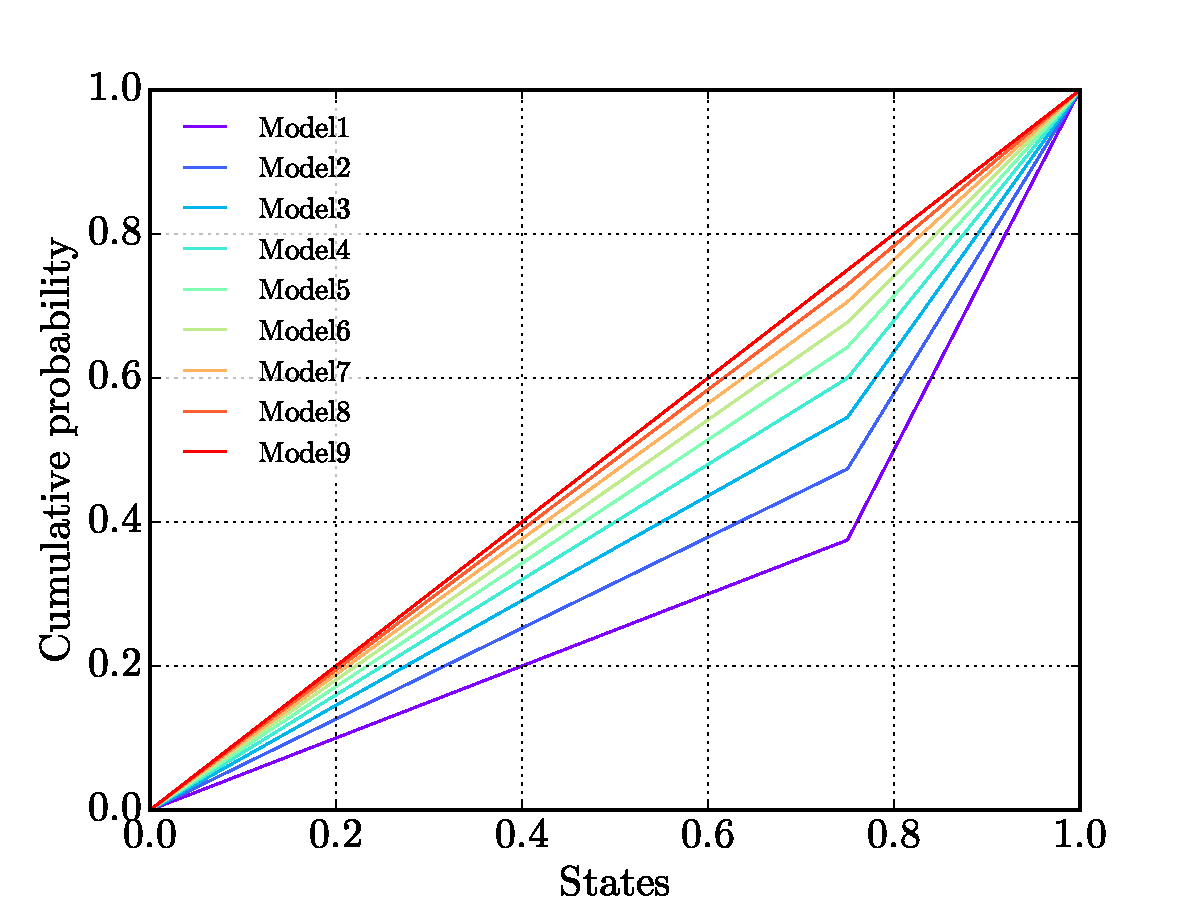
\includegraphics[width=\textwidth]{results/mc2_lorenz-curve}
        \caption{}
        \label{fig:mc2-lorenz}
    \end{subfigure}
    \hfill
    \begin{subfigure}{0.48\textwidth}
    	\centering
        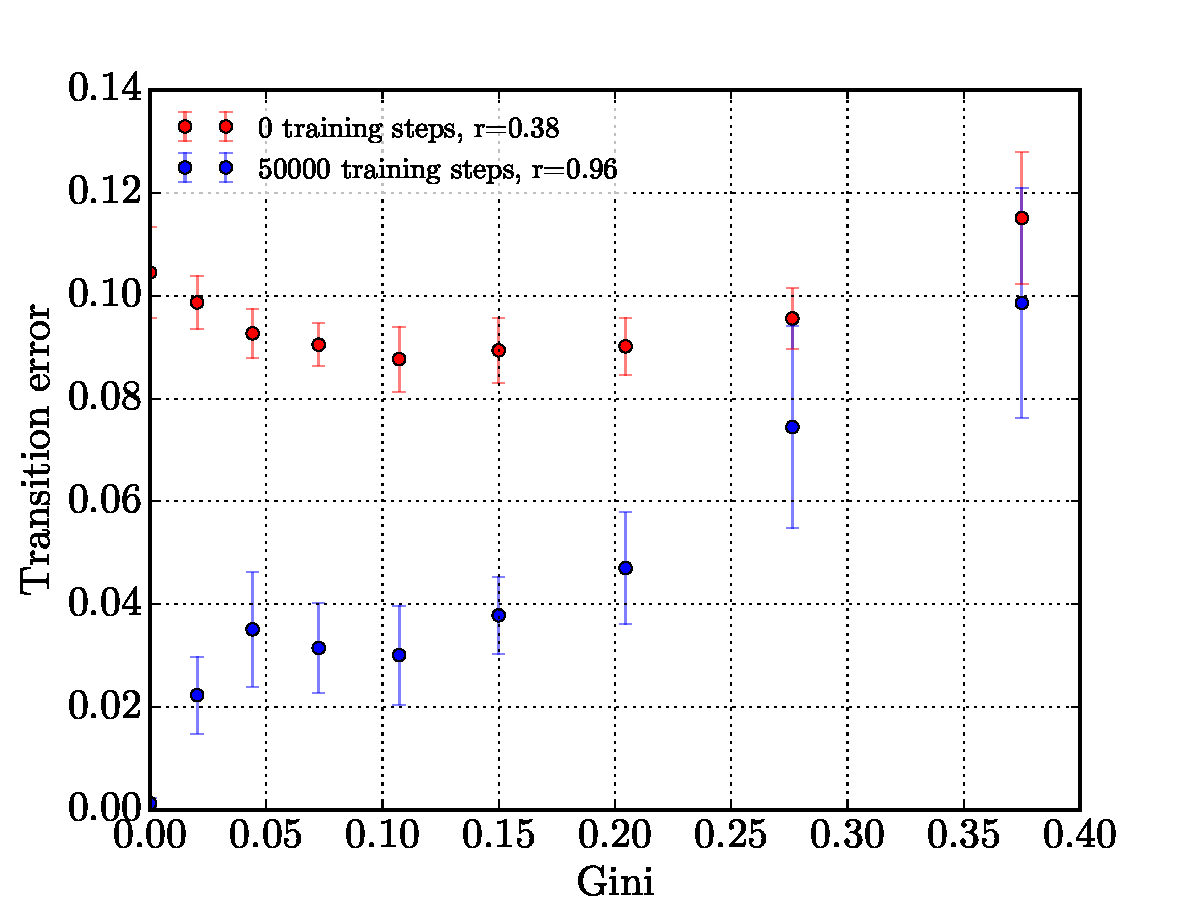
\includegraphics[width=\textwidth]{results/mc2_correlation_inequality_gini_train}
        \caption{}
        \label{fig:mc2-gini}
    \end{subfigure}
    \caption[Concentration of the stationary distribution]{Concentration of the stationary distribution. \textbf{a)} shows the Lorenz curves of all models from the second approach (figure \ref{fig:mc2-models}). The models differ in their concentration. In \textbf{b)} the Gini coefficients are calculated to quantify the concentration measure. They are put in relation with the performance of the models.}
    \label{fig:mc2-concentration}
\end{figure}

Figure \ref{fig:mc2-lorenz} shows the Lorenz curves for the models used above. The amount of concentration obviously differs between the different models. The relation between the performance $\varepsilon_M$ and the Gini coefficient $G$ is shown in figure \ref{fig:mc2-gini}. The effect is quite the same as it was before with the variance and the Kullback-Leibler divergence. Using the Gini coefficient, the correlation is $r_G = 0.96$. Therefore, the concentration of the distribution is just another perspective, but it does not explain more than the former approaches were doing. However, to evaluate the observations under a perspective of concentration had a decisive impact on the idea of the following \acs{ip}-hypothesis.

\subsection{IP-hypothesis}
\label{sec:ip-hyp}

The results from the previous section show a clear relation between the properties of the Markov chain and the performance. It is necessary to develop an explanation for this behavior and it remains to show that this behavior is robust, also for other Markov chains.

The hypothesis, which is suggested to explain the effect, focuses on the \acf{ip}. Therefore, the hypothesis is called \emph{\acs{ip}-hypothesis} in the following. Assume just $3$ states, $A$, $B$ and $C$. They correspond to input clusters at the excitatory neurons. The case is shown in figure \ref{fig:sorn-clusters}. Inhibitory neurons, input neurons and weights are not shown. Further, assume a stationary distribution

\begin{equation}
\pi = (\pi_A, \pi_B, \pi_C)^T = (0.8, 0.1, 0.1)^T.
\end{equation}

A simulation of a Markov chain with such a distribution and the three states could look like

\begin{equation}
A\;A\;A\;A\;A\;A\;A\;C\;B\;A.
\end{equation}

\begin{figure}[!t]
	\centering
	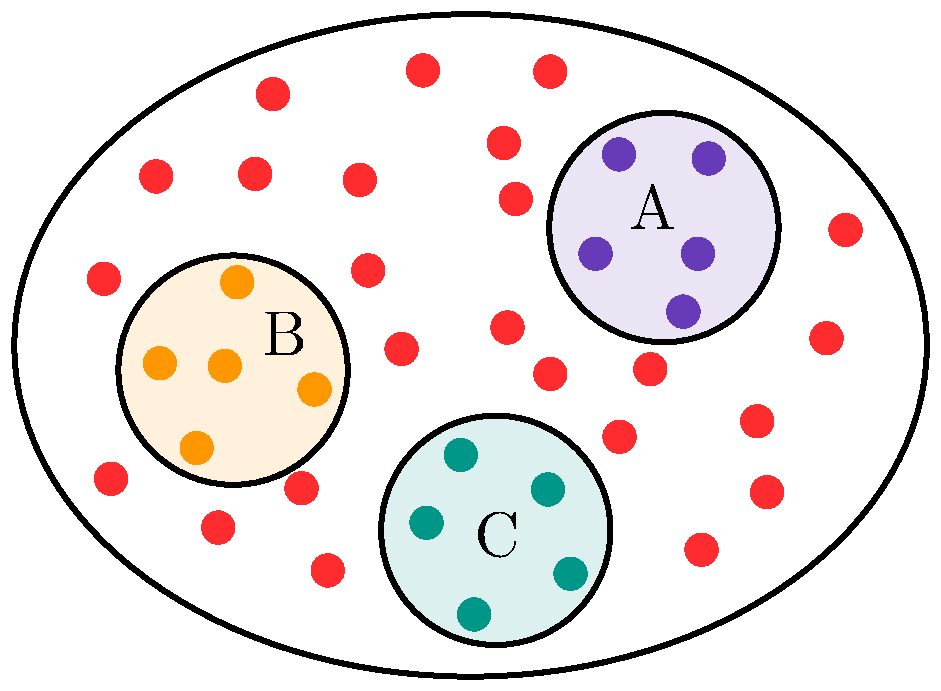
\includegraphics[width=0.65\textwidth]{results/sorn_cluster}
	\caption[Input clusters example]{Three input clusters as an example to illustrate \acs{ip}-hypothesis. If one cluster is not active for a longer time, neurons of that cluster will be active spontaneously and the chance for a misclassification increases.}
	\label{fig:sorn-clusters}
\end{figure}

It is necessary to remind the property of \acs{ip} regarding spontaneous activity, as it was shown in figure \ref{fig:intrinsic-plasticity} in section \ref{sec:ip}. If a neuron is not active for a long time, the threshold of that neuron is going down. If the threshold falls below zero, the neuron fires spontaneously. In the simulation, state $A$ and therefore neuron cluster $A$ is repetitively active in the network for a long time, due to its higher probability $\pi_A$. The threshold of the other neurons is going down at that time, because they are ideally not excited. That affects those neurons of cluster $B$ and $C$ in particular. Therefore, the chance rises that cluster $B$ or $C$ will be active spontaneously after some time.

Models with regular input patterns, meaning that the probabilities of the states are similar, have a better performance than those with irregular input patterns, where some states have a smaller probability than others. The \acs{ip}-hypothesis suggests that \acl{ip} is a cause for that observation. This hypothesis was tested in three steps:

\begin{itemize}
\item Apply different models and evaluate if the effects can be explained by the hypothesis.
\item Vary parameter $\bar H^\IP$ and evaluate if different levels of \acl{ip} influence the performance.
\item Vary parameter $\sigma_\IP$ and evaluate if the performance becomes more robust, independent of the model.
\end{itemize}

\paragraph{More models}

After the effect of the stationary distribution was shown, a bunch of different models was developed to test the \acs{ip}-hypothesis. In figure \ref{fig:mc-models-collection} four series of Markov chains are shown. They were all simulated with $T_\plastic = 50,000$.

The first series in figure \ref{fig:mc3-models}, model series III, is similar to the series of models II, presented in figure \ref{fig:mc1-models}. But while the previous models concentrated their probability at state $A$, in this case the probability is concentrated at states $B$, $C$ and $D$. Therefore, the chance that $A$ will be active spontaneously is increased, since this state is less active than the other states. The performance plot should show similar results to figure \ref{fig:mc2-performance-distance} and indeed, figure \ref{fig:mc3-performance-distance} shows that the results are very similar.

\begin{figure}[p]
    \centering
    \begin{subfigure}{0.85\textwidth}
    	\centering
        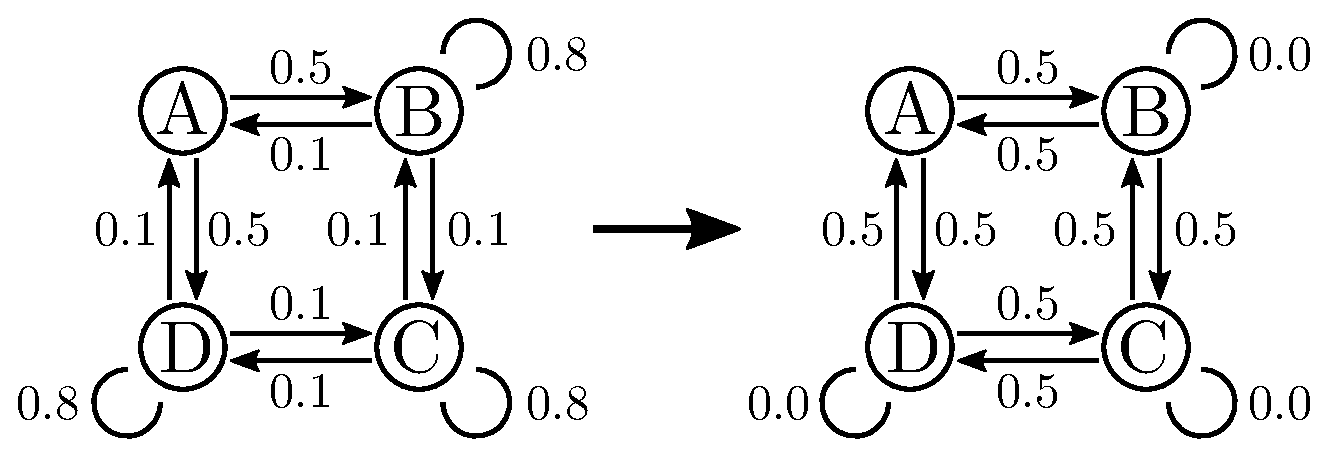
\includegraphics[width=\textwidth]{results/mc3_models}
        \vspace{-25pt}
        \caption{Model series III}
        \label{fig:mc3-models}
    \end{subfigure}
    \begin{subfigure}{0.85\textwidth}
    	\centering
        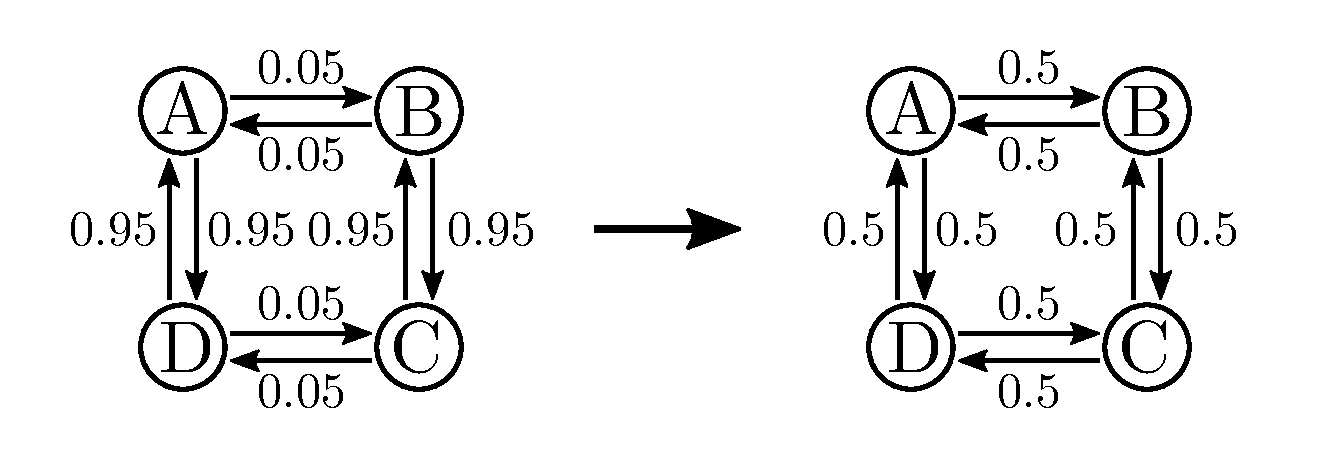
\includegraphics[width=\textwidth]{results/mc4_models}
        \vspace{-30pt}
        \caption{Model series IV}
        \label{fig:mc4-models}
    \end{subfigure}
    \begin{subfigure}{0.85\textwidth}
    	\centering
        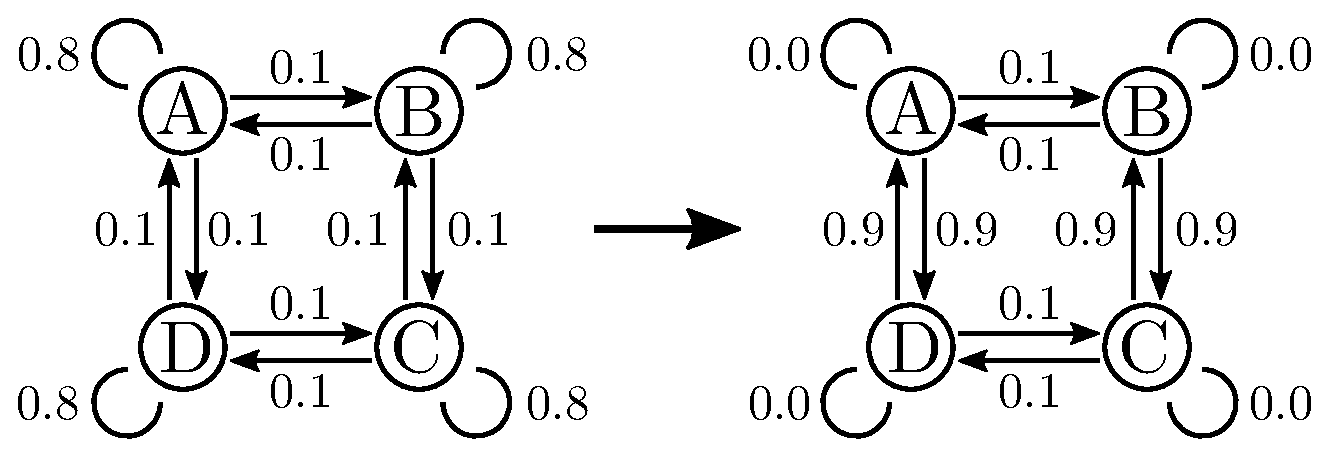
\includegraphics[width=\textwidth]{results/mc5_models}
        \vspace{-25pt}
        \caption{Model series V}
        \label{fig:mc5-models}
    \end{subfigure}
    \begin{subfigure}{0.85\textwidth}
    	\centering
        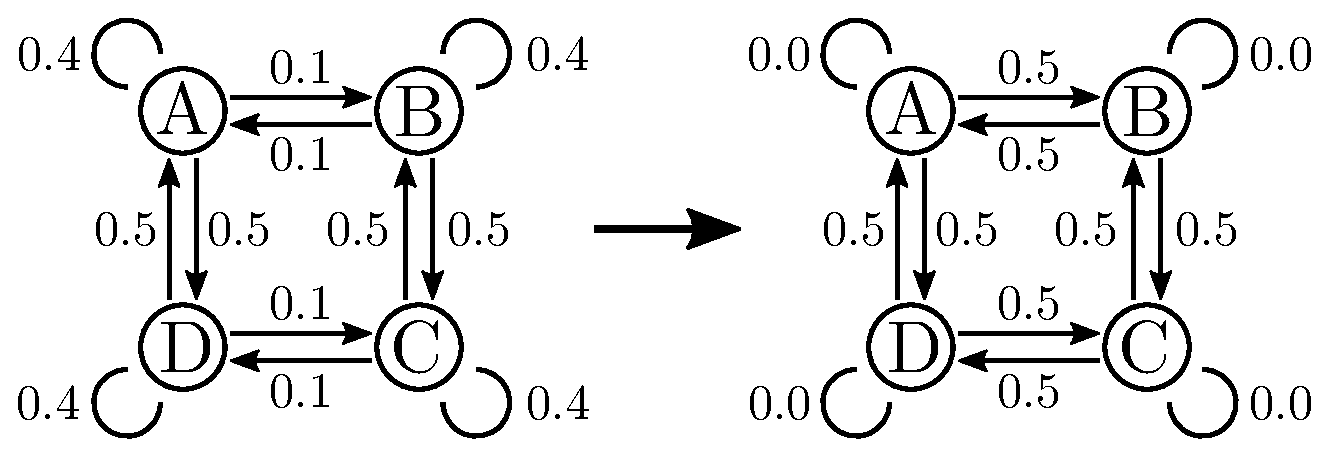
\includegraphics[width=\textwidth]{results/mc6_models}
        \vspace{-25pt}
        \caption{Model series VI}
        \label{fig:mc6-models}
    \end{subfigure}
    \caption[Four Markov model series to test the IP-hypothesis]{Four Markov model series to test the \acs{ip}-hypothesis. The first series in \textbf{a)} prefers state $B$, $C$ and $D$. Model by model, the self loop is decreasing and the probability to reach $A$ is increased. \textbf{b)} starts with a model which separates between the left and the right side. Series \textbf{c)} starts with a model where all four states are separated and changes step by step to a model where the right and left side are separated, which was the starting point in \textbf{b)}. Finally, in \textbf{d)} the first model separates between right and left and has some self loops additionally. This equals a middle model from \textbf{c)}. In series \textbf{b)}, \textbf{c)} and \textbf{d)} all models have the same stationary distribution with equal probability for every state.}
    \label{fig:mc-models-collection}
\end{figure}

\begin{figure}[p]
    \centering
    \begin{subfigure}{0.48\textwidth}
    	\centering
        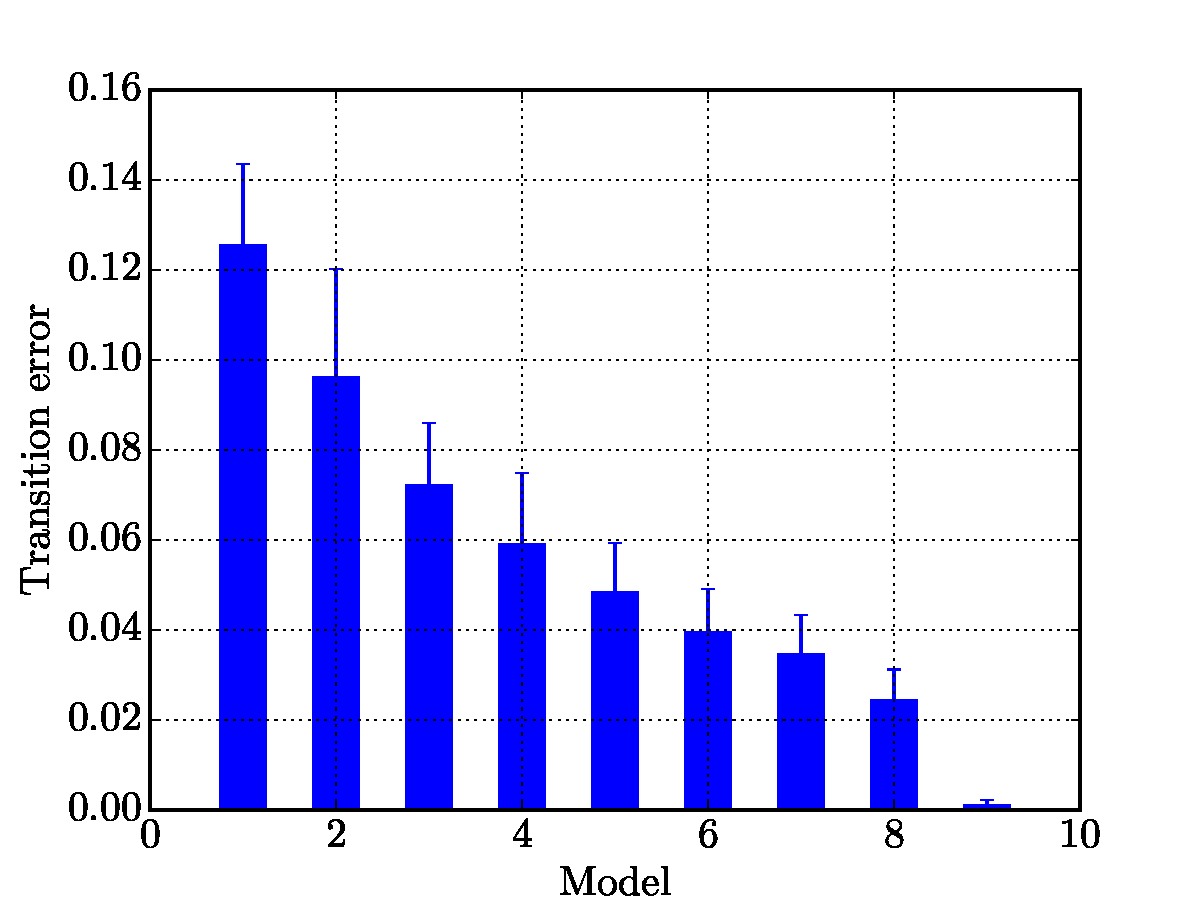
\includegraphics[width=\textwidth]{results/mc3_performance_distances}
        \caption{Model series III}
        \label{fig:mc3-performance-distance}
    \end{subfigure}
    \hfill
    \begin{subfigure}{0.48\textwidth}
    	\centering
        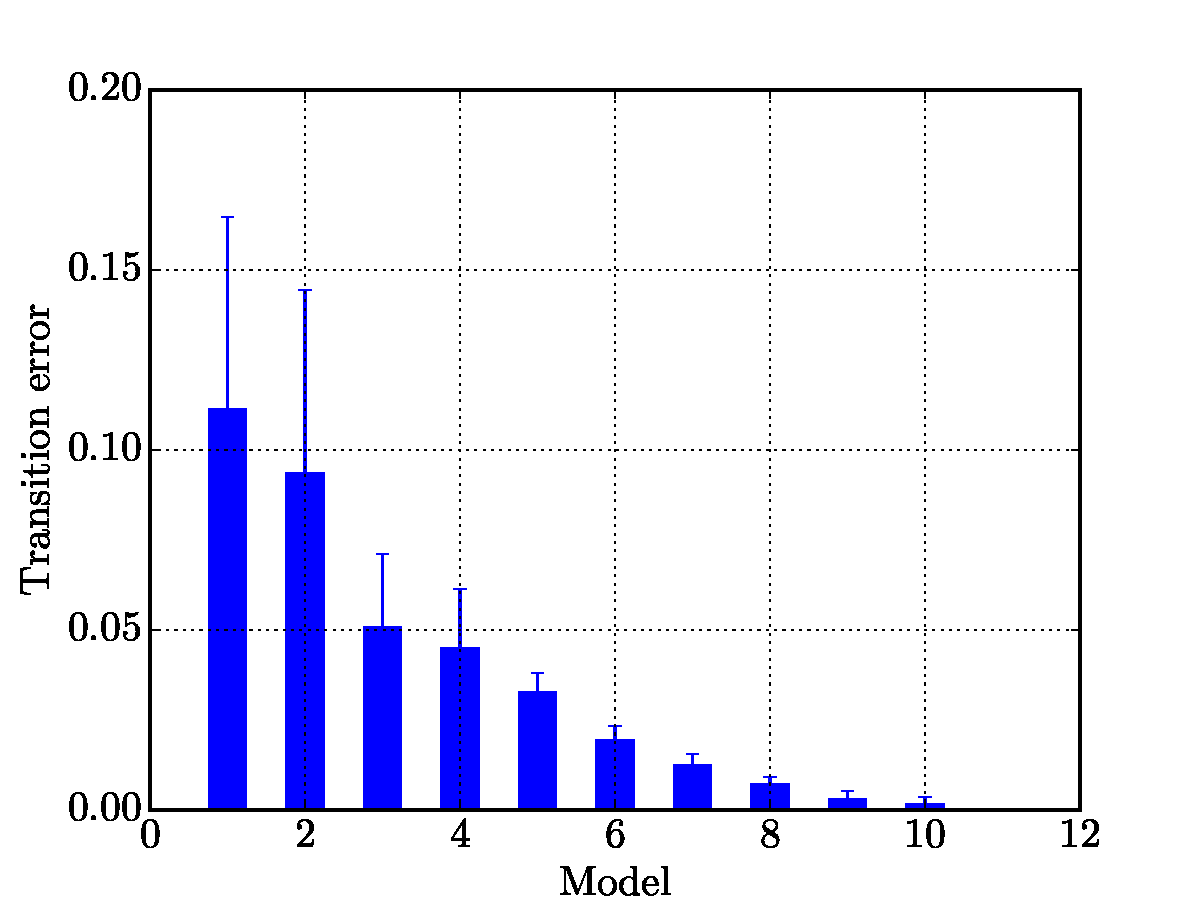
\includegraphics[width=\textwidth]{results/mc4_performance_distances}
        \caption{Model series IV}
        \label{fig:mc4-performance-distance}
    \end{subfigure}
    \begin{subfigure}{0.48\textwidth}
    	\centering
        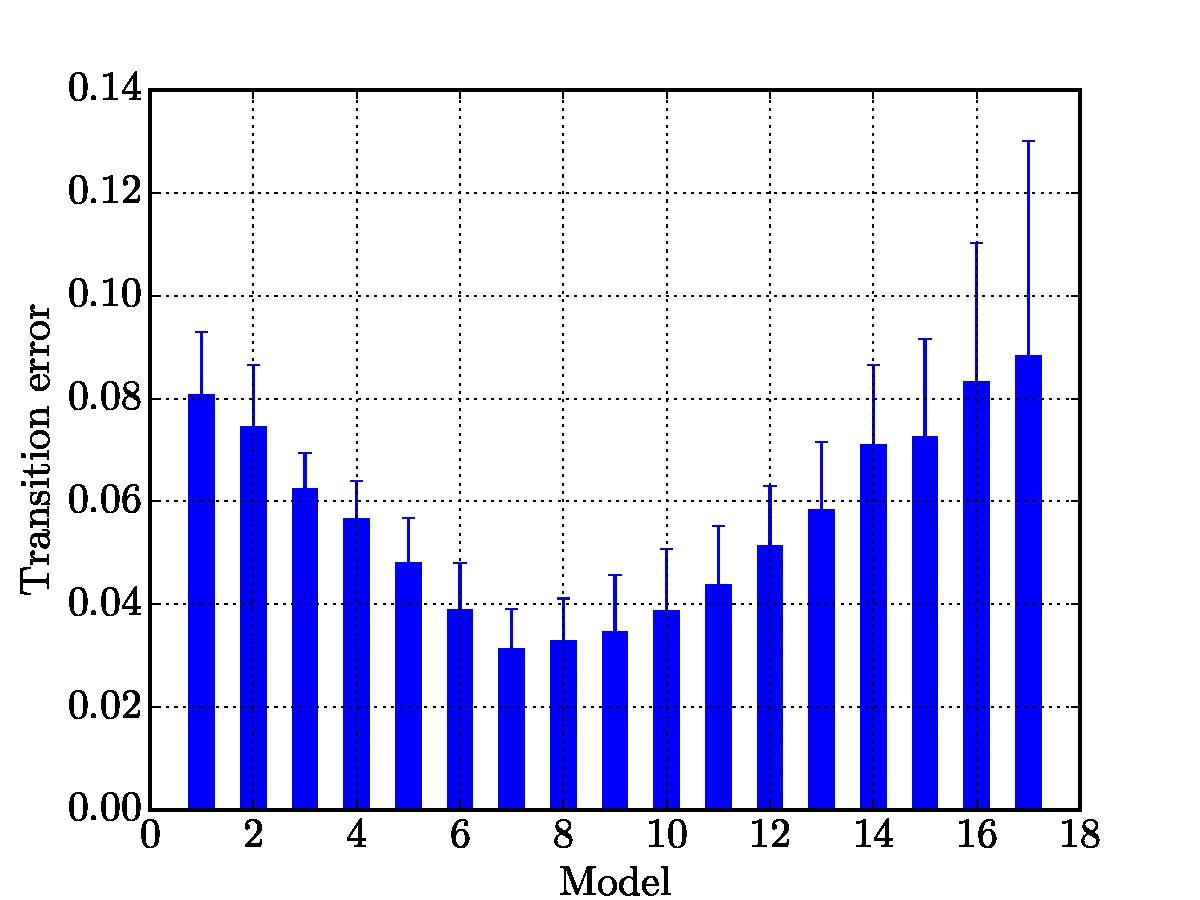
\includegraphics[width=\textwidth]{results/mc5_performance_distances}
        \caption{Model series V}
        \label{fig:mc5-performance-distance}
    \end{subfigure}
    \hfill
    \begin{subfigure}{0.48\textwidth}
    	\centering
        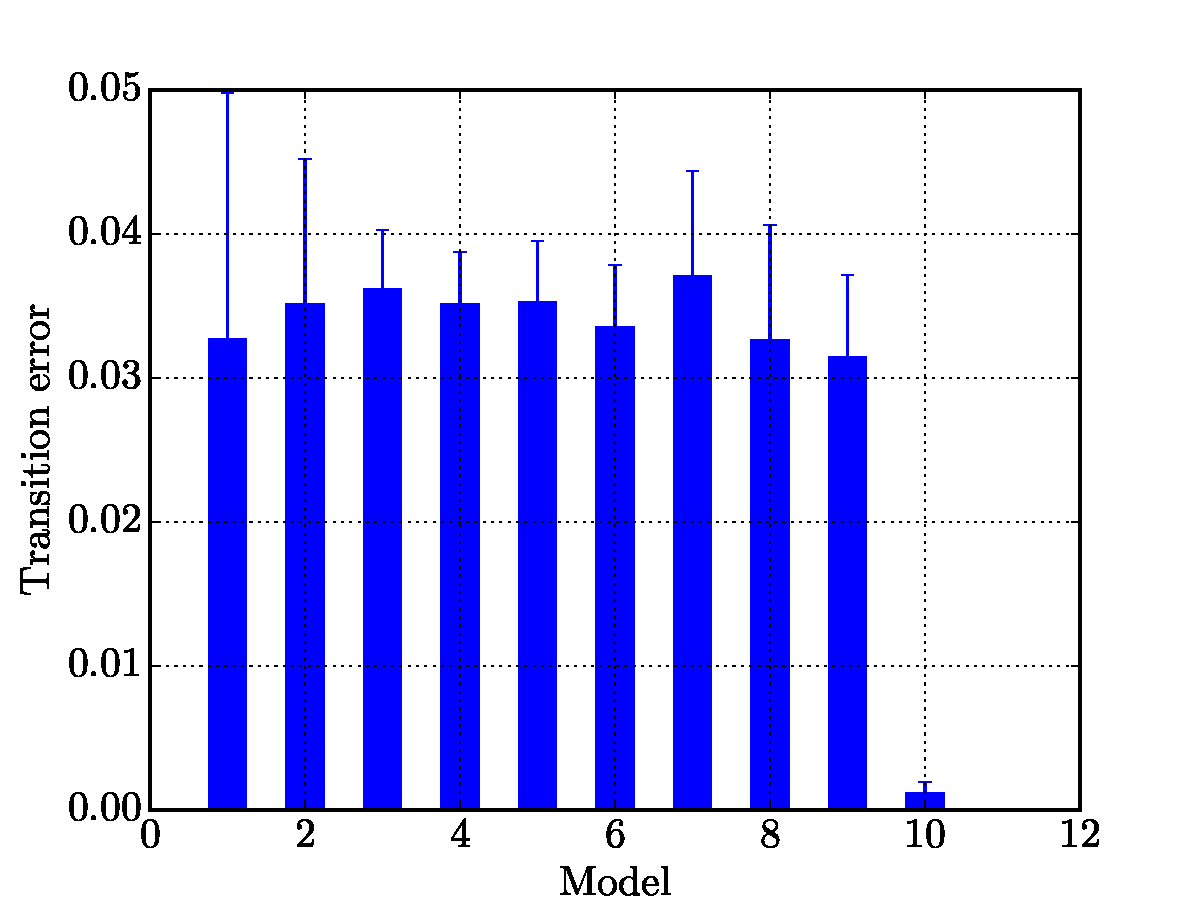
\includegraphics[width=\textwidth]{results/mc6_performance_distances}
        \caption{Model series VI}
        \label{fig:mc6-performance-distance}
    \end{subfigure}
    \caption[Performance of four Markov model series]{Performance of the four Markov model series from figure \ref{fig:mc-models-collection}. Model series III was divided into $9$ models, model series IV into $11$ models, model series V into $17$ models and model series VI into $11$ models. All four series follow the predicted behavior according to the \acs{ip}-hypothesis. The variance, the Kullback-Leibler divergence and the Gini coefficient, do not hold for prediction in cases \textbf{b)}, \textbf{c)} and \textbf{d)}, since every information and concentration measure is equal within every model series, while the performance differs significantly.}
    \label{fig:mc-series-performance}
\end{figure}

Model series IV, shown in figure \ref{fig:mc4-models}, separates the states $A$ \& $D$ and $B$ \& $C$ and join them step by step again. The interesting aspect of this approach is that the stationary distribution is absolutely equal for every model in this series, such that $\bm\pi = \left( \frac{1}{4}, \frac{1}{4}, \frac{1}{4}, \frac{1}{4} \right)^T$. At that point the predictors, namely the variance, Kullback-Leibler divergence and Gini coefficient, are the same for every model and would predict no differences in performance. On the other hand, the \acs{ip}-hypothesis predicts a change in performance. In the beginning, the probability to switch between the right and the left side is very small. Therefore, if one side is active, the chance increases that the other side will be active spontaneously. The more both sides are connected again, the better the performance should become. Figure \ref{fig:mc4-performance-distance} shows a clear decay in the \acs{mse} $\varepsilon_M$, which strongly supports the \acs{ip}-hypothesis. The down side of this result is, that the information and concentration measures do not longer hold as predictors. The information, contained in the stationary distribution is obviously not sufficient to predict the behavior.

Series V is more complex. In figure \ref{fig:mc5-models} the construction of the models is shown. It starts with a model where all four states are quite disconnected. It is expected that the performance is low in this case. The last model of this series equals the first model of the previous series. The model transforms from four separated parts to two separated parts. Comparing the performance of the first models and the last models in figure \ref{fig:mc4-performance-distance}, the error is quite similar. Therefore, it seems not very important if the chain is separated in four parts or in two parts. It seems to be more important how strongly the different parts are connected. Interestingly for the middle part, the error decreases. The middle model has a probability of $p_{x_i x_i} = 0.4$ for the self loop and $p_{AD} = p_{BC} = 0.4$. Probably the self loop increases the probability that the states can change between the right and the left side, since in some cases it stays in the same state and has another chance to switch. The first model suffers from a strong disconnection between all states. For those `islands' the self loop is not helpful. The last model has no self loops any more, which separates the the sides, as it was observed in the model series above. Note that the stationary distributions are the same for all models again, where each state has equal probability.

The last example, model series VI, is shown in figure \ref{fig:mc6-models} and again, all models in this series have the same distribution as before. In this case, the first model starts, where the third series was in its middle. At that point the performance was relatively good. The last model was already used before in many cases and is already known as a model which can be learned with high precision. It is predicted from what was observed before, that the self loop in the first models increase the probability that the states can switch the sides. The more the self loop probability is decreased, the more the direct connection between the two sides increase at the same time. This behavior should compensate the decrease in the self loops. It should result in a relatively similar performance for all models. Indeed, figure \ref{fig:mc6-performance-distance} shows that all models have a relatively constant and low error, where the last model is a little bit outstanding. Comparing this outlier model for example with \ref{fig:mc3-performance-distance}, indicates that this effect already happened before. A possible explanation is given in appendix \ref{sec:appendix:close}.

In conclusion, the \acs{ip}-hypothesis holds for all tested model series. In the following, the implementation of the \acl{ip} mechanism from equation \eqref{eq:hip-ind} is tested for different parameters to come closer to an understanding of how \acs{ip} works.

\paragraph{Influence of parameter $\bar H^\IP$}

\begin{figure}[!t]
    \centering
    \begin{subfigure}{0.48\textwidth}
    	\centering
        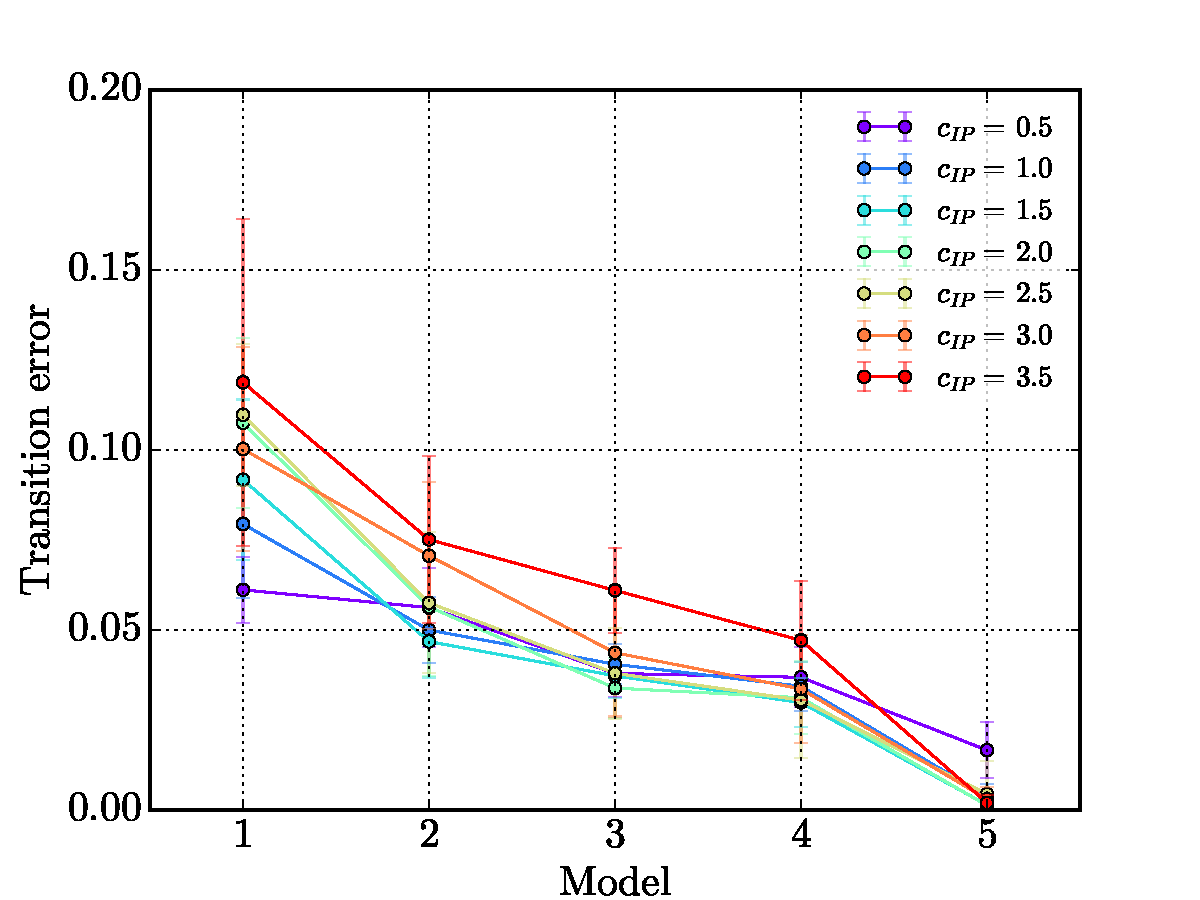
\includegraphics[width=\textwidth]{results/h_ip}
        \caption{}
        \label{fig:hip-allmodels}
    \end{subfigure}
    \hfill
    \begin{subfigure}{0.48\textwidth}
    	\centering
        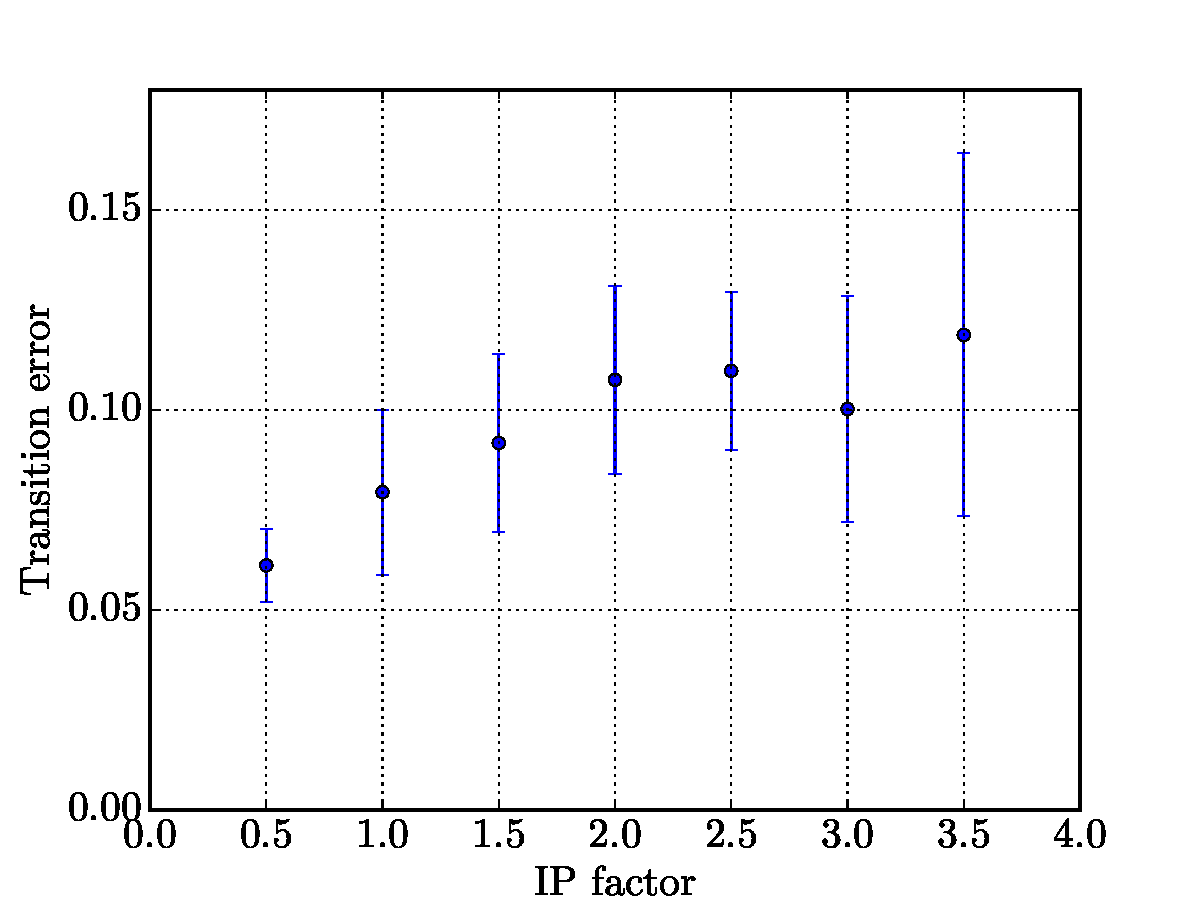
\includegraphics[width=\textwidth]{results/h_ip_model1}
        \caption{}
        \label{fig:hip-model1}
    \end{subfigure}
    \begin{subfigure}{0.48\textwidth}
    	\centering
        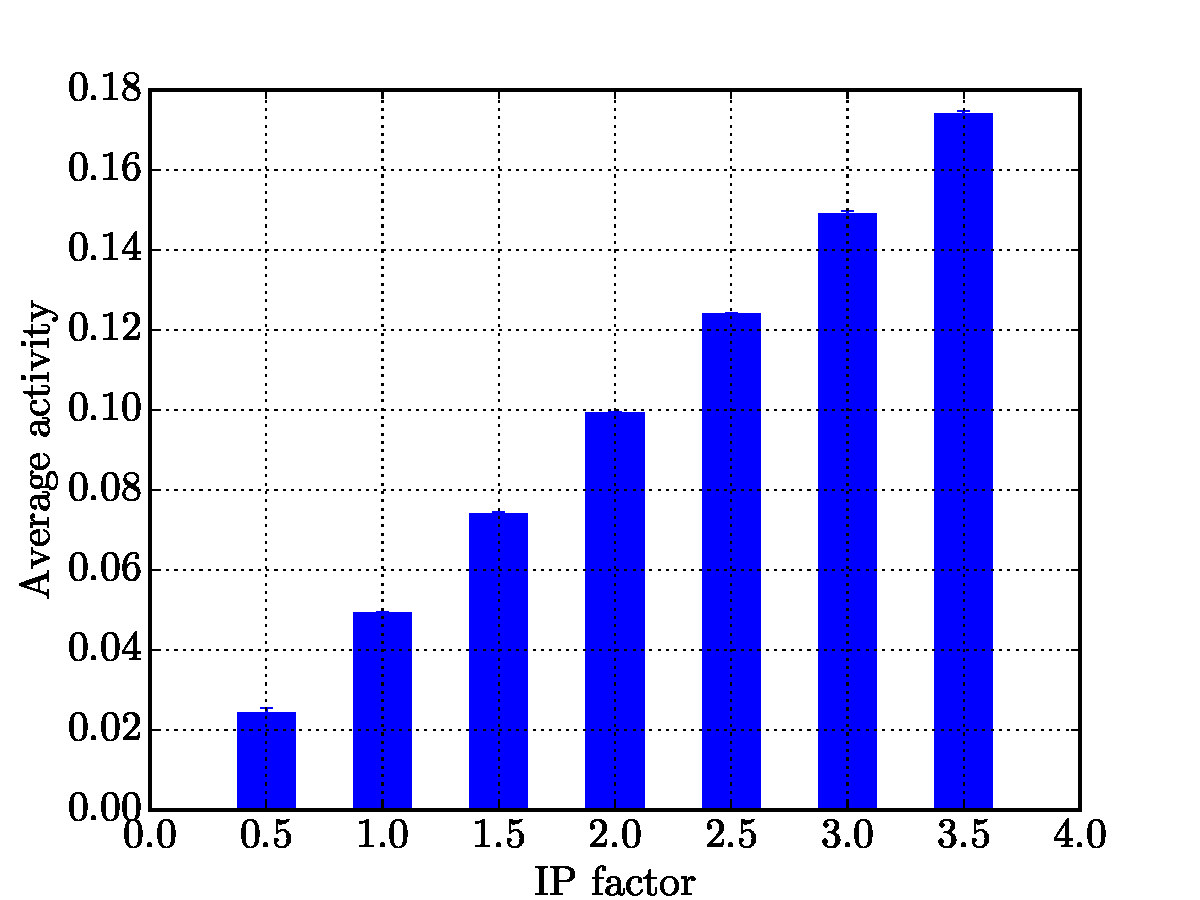
\includegraphics[width=\textwidth]{results/h_ip_activity_model1}
        \caption{}
        \label{fig:hip-activity-model1}
    \end{subfigure}
    \hfill
    \begin{subfigure}{0.48\textwidth}
    	\centering
        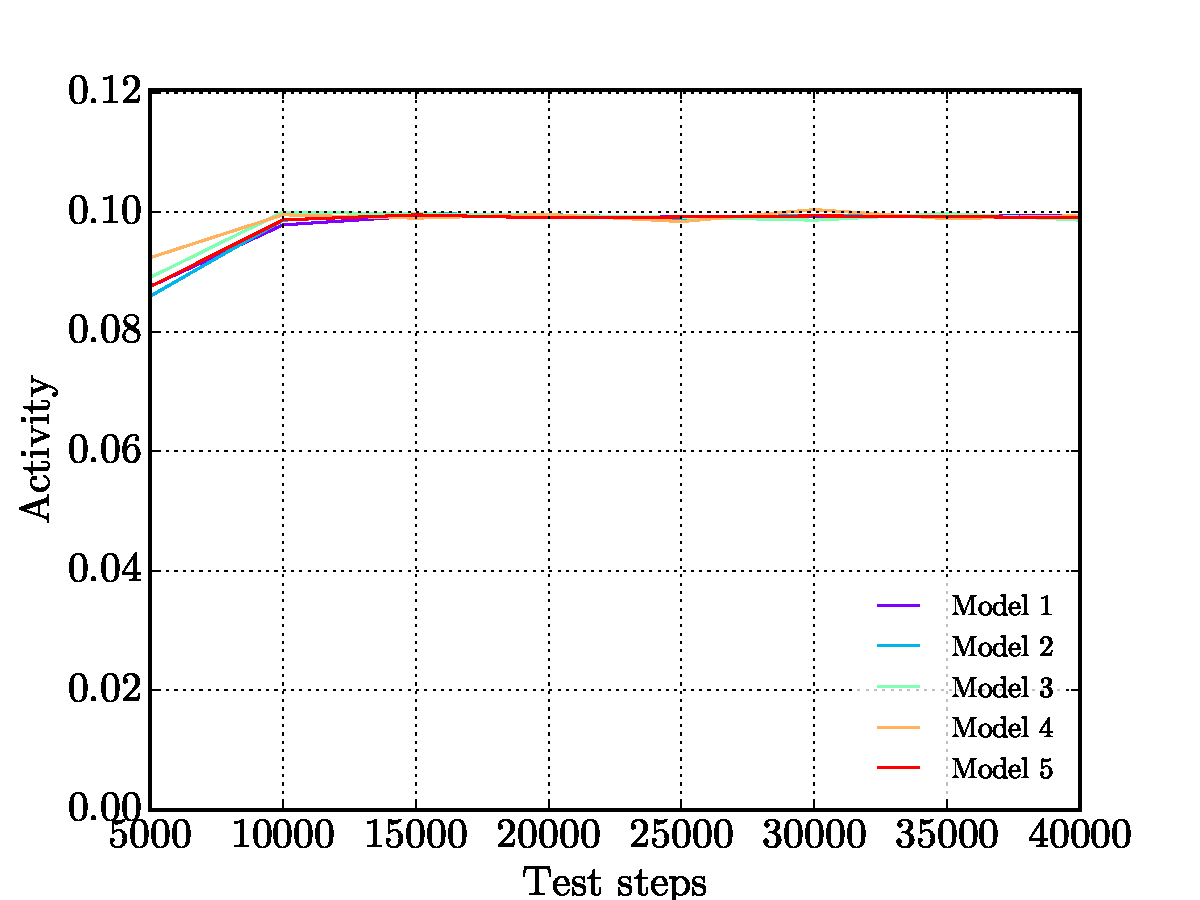
\includegraphics[width=\textwidth]{results/h_ip_test_traces_activity}
        \caption{}
        \label{fig:hip-activity-trace}
    \end{subfigure}
    \caption[Influence of the IP target rate]{Influence of the target rate on model series II, divided into $5$ models. The target rate factor $c_\IP$ was varied from $0.5$ to $3.5$ in steps of $\Delta c_\IP = 0.5$. \textbf{a)} shows the behavior for all models, where the performances of the first models seem to be influenced by the target rate. In \textbf{b)} a further investigation of the very first model was done, since effects are expected to be most clear for that model. It shows that the target rate has an effect on the performance for that model, where $p$-values are given in table \ref{tb:hip-ttests}. The average activity of the network for the first model is plotted in \textbf{c)}, showing that the target rate directly influences the activity in the network. In plot \textbf{d)} the activity for $c_\IP = 2.0$ is shown over the whole testing phase for all models. After a short burn in phase, the activity stays very constant. Note that this plot bases only on a single simulation. In all cases, errorbars indicate standard errors.}
    \label{fig:hip-influence}
\end{figure}

If the \acl{ip} is responsible for the performance differences between the models, then a change of the parameters of the \acs{ip} mechanism should be reflected in the performance of the models. $\bar H^\IP = 2\cdot N^U/N^E$ is the main factor inducing spontaneous activity. The lower the target rate $\bar H^\IP$, the less spontaneous activity is present and vice versa. Models, where specific states are less probable, should profit from a lower target rate. Those states can stay silent for a longer time until \acl{ip} will spontaneously activate them. Since the \acs{ip} is the only source for activity in the testing phase, it is somehow problematic to change the parameter. The \acs{ip} mechanism directly changes the average activity in the network. It cannot be excluded that it is the activity level in general rather than the threshold of the mechanism which influences changes in performance. For the simulation a parameter $c_\IP$ was used, such that $\bar H^\IP = c_\IP \cdot N^U/N^E$ where $c_\IP = 2$ is the default value.

However, the results with different $c_\IP$ values are shown in figure \ref{fig:hip-influence}. It was applied to the systematic model series II from figure \ref{fig:mc2-models}. For simplicity of the presentation of the results in the plots, the series was created with just $5$ models in opposite to results shown in figure \ref{fig:mc2-kl}, where the series was applied with $9$ models. The first plot in figure \ref{fig:hip-allmodels} shows the performance of all $5$ models and all $c_\IP$ values. As expected from the results before, the error decreases when state $A$ is less isolated. In those models, where state $A$ is highly isolated, the \acs{ip} target rate influences the performance of the models. For evaluation, the first model was chosen. This model has the lowest probability to reach state $A$ and therefore the target rate should have the highest influence to that model. In figure \ref{fig:hip-model1} the performance results for the first model are shown, depending on the \acs{ip} factor $c_\IP$. It seems that there is a positive correlation between the parameter and the error $\varepsilon_M$, at least between $c_\IP = 0.5$ and $c_\IP = 2.0$. In table \ref{tb:hip-ttests}, t-tests between all errors value were applied, showing that the intuition is correct. The main effect happens before $c_\IP = 2.0$, afterwards no significant changes can be observed. This results supports the \acs{ip}-hypothesis, even though the effects seem to decay very fast with further models.

\begin{table}[!t]
\centering
\begin{tabular}{c|ccccccc}
$c_\IP$ & $1.0$ & $1.5$ & $2.0$ & $2.5$ & $3.0$ & $3.5$ \\
\hline
$0.5$ & \makecell{$\mathbf{1.08\cdot 10^{-3}}$\\ \starsSS} & \makecell{$\mathbf{2.46\cdot 10^{-6}}$\\ \starsSSS} & \makecell{$\mathbf{1.12\cdot 10^{-9}}$\\ \starsSSS} & \makecell{$\mathbf{6.61\cdot 10^{-12}}$\\ \starsSSS} & \makecell{$\mathbf{1.37\cdot 10^{-6}}$\\ \starsSSS} & \makecell{$\mathbf{3.44\cdot 10^{-6}}$\\ \starsSSS} \\
$1.0$ & & \makecell{$0.085$\\ \starsNS} & \makecell{$\mathbf{3.62\cdot 10^{-4}}$\\ \starsSSS} & \makecell{$\mathbf{4.01\cdot 10^{-5}}$\\ \starsSSS} & \makecell{$\mathbf{0.014}$\\ \starsS} & \makecell{$\mathbf{1.41\cdot 10^{-3}}$\\ \starsSS} \\
$1.5$ & & & \makecell{$\mathbf{0.040}$\\ \starsS} & \makecell{$\mathbf{0.011}$\\ \starsS} & \makecell{$0.310$\\ \starsNS} & \makecell{$\mathbf{0.025}$\\ \starsS} \\
$2.0$ & & & & \makecell{$0.750$\\ \starsNS} & \makecell{$0.395$\\ \starsNS} & \makecell{$0.343$\\ \starsNS} \\
$2.5$ & & & & & \makecell{$0.236$\\ \starsNS} & \makecell{$0.433$\\ \starsNS} \\
$3.0$ & & & & & & \makecell{$0.139$\\ \starsNS} \\
\end{tabular}
\vspace{5pt}
\caption[p-values of performance differences between $\bar H^\IP$ values]{$p$-values of performance differences for simulations with different target rate factors $c_\IP$ for model $1$. Bold values indicate significant differences with $p \le 0.05$.}
\label{tb:hip-ttests}
\end{table}

Figure \ref{fig:hip-activity-model1} shows the average activity for the first model, depending on the target rate. It is clear from that plot that $\bar H^\IP$ directly influences the amount of activity, which is defined as the number of spiking excitatory neurons $n_{\text{spiking}}(t) = |\ \{ i \in \{1, ..., N^E\} \,:\, x_i(t) = 1\} |$ divided by the total number of excitatory neurons $N^E$ at a specific point in time $t$. Additionally, for a fixed $c_\IP$, the activity is very stable and independent of the model, as shown in figure \ref{fig:hip-activity-trace}. It shows the activity over the testing phase for $c_\IP = 2.0$ for a single simulation. Note that this activity is not averaged. The activity differences could potentially influence the performance directly. To exclude effects from the amount of activity in the networks, noise could be implemented to hold a specific level of activity. This approach is considered in the discussion in section \ref{sec:discuss-ip}. 

However, even though the effects are not very strong and possibly influenced by the activity, in tendency, they support the \acs{ip}-hypothesis.

\paragraph{Influence of parameter $\sigma^\IP$}

\begin{figure}[!b]
	\centering
	\includegraphics[width=0.85\textwidth]{results/h_ip_range}
	\caption[Influence of the IP target rate range]{Variation of \acs{ip} target rate range $\sigma^\IP$ applied to model series II, divided into $5$ models. The target rate range was varied from $0.0$ to $0.03$ with steps of $\Delta \sigma^\IP = 0.05$. Error bars indicate standard errors. The performance is independent from the chosen target rate range for all models.}
	\label{fig:hip-range}
\end{figure}

\textcite{hartmann2015s} have shown that the network performs more robust if the target rate is not the same for every neuron. Therefore, in this thesis the parameter $\sigma^\IP$ was introduced in section \ref{sec:ip-mod} and chosen as $0.01$, pursuant to their suggestion. The parameter determines the range, how much a target rate of a specific neuron can differ from the average target rate $\bar H^\IP$. According to \textcite{hartmann2015s}, the performance should decrease if $\sigma^\IP$ is lower than $0.01$ or even zero. The latter case with $\sigma^\IP = 0$ corresponds to the rule \textcite{lazar2009sorn} used in the initial \acs{sorn}. Beside reproducing the behavior for $\sigma^\IP < 0.01$, it also remains to show what happens if $\sigma^\IP$ is increased above $0.01$ and to evaluate the results in context of the \acs{ip}-hypothesis.

To keep it comparable with the variation of the $\bar H^\IP$ parameter, also the systematic model series II from figure \ref{fig:mc2-models} was applied, divided into $5$ models. Figure \ref{fig:hip-range} shows the  performance of all $5$ models for all $\sigma^\IP$ values. The differences in the performance are not significant ($p > 0.05$) for all models, except one, where the difference between $\sigma^\IP = 0.02$ and $\sigma^\IP = 0.03$ in the first model is significant with $p = 0.035$. But since the significance level is low and all other $20$ comparisons for the first model alone are non-significant, the results from \textcite{hartmann2015s} could not be reproduced. Contrary to their findings, the present findings suggest no effect below $\sigma^\IP < 0.01$, nor is an effect above $\sigma^\IP > 0.01$. The result suggests that the initial \acs{ip} rules from \textcite{lazar2009sorn} is sufficient. Regarding the \acs{ip}-hypothesis, the $\sigma^\IP$ parameter seems to have no or at best a very small influence on the less probable states. Since the arguments of \textcite{hartmann2015s} for introducing $\sigma^\IP$ are plausible, perhaps further research is necessary to understand in which cases a variation of the parameter for the neurons can increase the robustness. A suggestion for another approach is given in the discussion section, in subsection \ref{sec:discuss-ip}.

\paragraph{Other parameters}

Two other aspects should be considered: the learning rate $\eta_\IP$ and the connectivity of the network.

First, $\eta_\IP$ is the learning rate of the \acl{ip}. The higher the learning rate, the faster the network reaches its target rate $\bar H^\IP$. It should not influence the performance of the models, since the burn in phase was always excluded from evaluation. However, the effect of $\eta_\IP$ regarding the burn in phase is considered in appendix \ref{sec:appendix:eta}.

Beside effects from the \acl{ip}, it is also necessary that the neurons are adequately connected. It could be that this assumption does not hold. Under some conditions, the structure of the network may be rather good, under others rather bad. An approach to test if such effects possibly occur, is to vary the connectivity of the network. It is the average number of connections between the excitatory neurons, denoted by $\lambda^W = \rho \cdot N^E$, where $\rho = 0.1$ by default. If $\rho$ is changed, the number of average connections changes. According to the appendix section of \textcite{lazar2009sorn} a sparse network with about $10\%$ of connections performs best. It means that every neuron is connected with $10\%$ of the other excitatory neurons in the network. If the number of connections is too high, there is a higher risk that the activity in the network grows without bounds. In context of the \acs{ip}-hypothesis, it is probably worth to vary the connectivity $\rho$ again in the setting of the Markov chain approach. The results are shown in appendix \ref{sec:appendix:connectivity}. It was possible to reproduce former results and a connectivity of $10\%$ seems to fit well, also in context of the \acs{ip} hypothesis. If the connectivity is too low or too high, the error increases.





\section{Discussion}

\ACL{sorn}s are a promising approach in modeling brain processes. \acs{sorn} extends randomly initialized reservoir networks with binary threshold neurons by using three biologically motivated plasticity mechanisms. It has already been shown that this self-organizing network outperforms static reservoir networks and is able to reproduce experimental findings, shown in section \ref{sec:prop-sorn}. \textcite{lazar2009sorn} stated that many basic mechanisms, like plasticity mechanisms, are more and more researched. Even though those mechanisms still lack a deep understanding, it is highly interesting how they work together in a balanced system. The hope is to get a deeper understanding of basic processes of dynamic non-linear systems, like the brain. 

Since the number of neurons in the network is relatively small, in a scale of hundreds, the applications are limited to sensory or short-term processes. Indeed, when \acl{stdp} was active in the testing phase, the network tends to forget the stored information by time. It should be possible to build larger networks using \acs{sorn}, for example in combination with cell assemblies. At present, cell assemblies are often build with static reservoir networks, but first dynamic approaches already exist \parencite{dasgupta2015self, tetzlaff2015use}.

However, this thesis focuses on a small sized network and its properties. The combination of the plasticity rules led to the interesting finding, that different input patterns highly influence how well the network is able to store and reproduce this input. Furthermore, it was hypothesized that \acl{ip} plays in important role for those results.

\subsection{Perspectives on SORN}

There are severals mathematical perspectives to interpret \acs{sorn}. Three variants could be collected.

\begin{itemize}
\item Trajectory in high dimensional space: The (spontaneous) activity in the network, with its $N^E$ neurons, can be seen as a trajectory in an $N^E$-dimensional space. This perspective has similarities with kernels. The input is transformed in a high dimensional time-dependent feature space, which was already discussed in section \ref{sec:res-net}.
\item \acl{mcmc} sampling: If the time-dependent input pattern is modeled with a Markov chain, the network learns from Markov chain samples. Furthermore, in testing phase, the network reproduces those samples.
\item Statistical estimator: Again, if \acs{sorn} is trained, using a distribution for the input neurons, the network can be seen as an estimator for this distribution. The parameters of the network determine the quality of the estimator. If the underlying Markov chain is unknown, it can be estimated by the (spontaneous) activity patterns of the network.
\end{itemize}

Regarding the sampling perspective, the samples from the Markov chain could be biased while training. According to the law of large numbers, after a long time the average converges to the Markov distribution. But in finite time steps, it is possible to have large runaways. Therefore, it is not guaranteed that the network was trained with a perfect Markov chain. This effect could be stronger in those networks, where some states are repeated very often. To put it in other words, in testing phase, the network does not reproduce the Markov chain, it reproduces the \emph{samples} from the training phases, which were samples from the Markov chain. However, since the results are averaged over $\Nsim$ runs and the standard error was calculated, this influence is assessable.

\subsection{Reverse learning effect}

\textcite{hartmann2015s} applied different probabilities to $8$ input states. States $A$, $B$, $C$ and $D$ occurred with a probability between $\frac{0.1}{4} = 0.025$ and $\frac{0.9}{4} = 0.225$ for each state. In contrary, states $E$, $F$, $G$ and $H$ were active with the reverse probability between $\frac{0.9}{4}$ and $\frac{0.1}{4}$. The probabilities were changed in steps of $0.1$. In figure \ref{fig:reverse-effect} the results are shown. Between $0.2$ and $0.8$, the network was able to reproduce the initial probabilities with a small amount of over representation. But at $0.1$/$0.9$, the effect was reversed and the variance increased. \textcite{hartmann2015s} argued that this effect is due to `pathological network dynamics', while a specific explanation was missing. It is suggested that the \acs{ip}-hypothesis is able to explain the reverse effect. Probably, the states were changing fast enough and avoiding distorting spontaneous activity in the range between $0.2$ and $0.8$. After that, it is likely that the threshold becomes smaller than zero, before the state is activated again according to the rule.

\begin{figure}[!t]
    \centering
    \begin{subfigure}[t]{0.48\textwidth}
    	\centering
        \includegraphics[width=\textwidth]{discussion/reverse-effect}
        \caption{States $A$, $B$, $C$ \& $D$ and $E$, $F$, $G$ \& $H$  were learned with probabilities between $0.1$ and $0.9$. At the extreme points, a reverse effect in the representation was observed \parencite[figure 4c]{hartmann2015s}. It can possibly be explained with \acl{ip}.}
        \label{fig:reverse-effect}
    \end{subfigure}
    \hfill
    \begin{subfigure}[t]{0.48\textwidth}
    	\centering
        \includegraphics[width=\textwidth]{discussion/ex-to-ex}
        \caption{The fraction of excitatory-to-excitatory connections, where $w_{ij} > 0$ during plastic training, stabilizes after about $20,000$ steps \parencite[figure 1d]{hartmann2015s}. It is assumed to correspond to the error decay in the first $20,000$ steps of training.}
        \label{fig:ex-to-ex}
    \end{subfigure}
    \caption[Reverse learning effect and fraction of excitatory-to-excitatory connections]{Reverse learning effect and fraction of excitatory-to-excitatory connections from \textcite{hartmann2015s}.}
    \label{fig:hartmann-figs}
\end{figure}

\subsection{Biological plausibility}

The question arises if the differences in the learning performance are due to \acs{sorn} alone or if there are indications that this behavior can also be observed in experiments where responses from mammal brains are recorded. In psychology, an experimental design, called \emph{oddball paradigm}, is often used for recording the neural behavior of time-dependent stimulus patterns. It consists of a \emph{standard} stimulus, which is repeated very often, and a \emph{deviant}, which breaks the previous stimuli. If the electrophysiological or magnetophysiological activity of the brain is recorded, a deviant elicits an \acfi{erp} or more specific a \acfi{mmn}. The electro- or magnetophysiological activity differs significantly from normal activity when a deviant stimulus is presented \parencite{naatanen1978early}.

The processes, underlying the \acs{mmn} mechanism, is assumed to be pre-attentive and on a sensory memory level \parencite{tiitinen1994attentive}. While the \acs{mmn} was obtained with simple stimulus rules, \textcite{paavilainen2007preattentive} and \textcite{bendixen2008rapid} were able to show that also more complex stimulus rules can be learned and detected by the brain. Such a rule is shown in figure \ref{fig:oddball-rule}. The learning of those complex rules is not accessible to attentive processing, which emphasizes that the detection mechanisms is connected to processing on sensory level. As already stated above, \acs{sorn} has also characteristics of a sensory or short-term memory. Thus, a parallel between those experiments with humans and the simulation can be drawn. Furthermore, in a more broad perspective, the difference between standard and deviant stimuli can be seen as stimuli which are more probable or less probable, respectively. The input patterns can therefore be modeled as Markov chains, which was done by \textcite{mill2011neurocomputational}. They found that the way the deviants, or less probable states, are represented in the network, highly depends on the parameters of the system, which was also found in this thesis.

\begin{figure}[!t]
	\centering
	\includegraphics[width=\textwidth]{discussion/oddball-rule}
	\caption[Complex rule used in oddball paradigm]{Complex rule with auditory stimuli used in oddball paradigm \parencite[figure 1]{paavilainen2007preattentive}. Long tones are followed by high tones (high frequency $f$) and short tones are followed by low tones. $S$ indicates a standard stimuli, fitting to the rules, $D$ indicates a deviant, breaking the rule.}
	\label{fig:oddball-rule}
\end{figure}

To the best of the authors knowledge, there are no experimental findings which either clearly supports the exact findings, nor rejects it. However, there is a lot of evidence that less probable stimuli are processed in a special way. In future research, it would be an interesting approach to use the oddball paradigm to train different stimuli patterns to the brain using Markov chains. Results from such an experiment would probably reveal if the effect from the simulation also appears in natural networks.

Another biological relation can be found regarding the plastic training. In the results section, figure \ref{fig:mc1-training} shows that the network needs about $20,000$ steps of plastic training, until the performance becomes stable and further training does not influence the performance any more. Interestingly, there seems to be a parallel to the observation that the fraction of excitatory-to-excitatory connections stabilizes after some time. The fraction designates how many weights stay with a weight of $w_{ij} > 0$ during plasticity training. Many weights, which are not necessary for the input pattern, decay to zero or close to zero, due to \acs{stdp}. This effect is known to occur in natural networks \parencite{yasumatsu2008principles}. In figure \ref{fig:ex-to-ex} a plot from \textcite{hartmann2015s} is shown. It takes about $20,000$ steps of training until the stable fraction was reached. This corresponds to the training time of the network and possibly explains the ceiling effect of training steps. As long as non-necessary connections exist, the input pattern cannot be reproduced very well. A ceiling is reached, when the fraction stabilizes. At that point no further increase in performance should be possible.

As already mentioned in section \ref{sec:prop-sorn}, \textcite{zheng2013network} extended a \acs{sorn} with structural plasticity. After every step, with a low probability, new connections were established. With this mechanism it should be possible to extend the learning phase slightly. It could possibly also reduce the effects due to the \acs{ip} mechanism. Furthermore, while initializing the connections, a stochastic component to the connectivity of every neuron could be added. The connectivity $\lambda^W$ would stay the same as before, but it would become the mean connectivity per neuron instead of a fixed connectivity per neuron. A stochastic component with a specific distribution could add variation to every neuron.

\subsection{Markov chains}

Directly connected to the former suggestion, it would be interesting to apply multi-state Markov chains. Currently, only one state is active at a specific point in time. This holds for the plastic and no-plastic training as well as for the testing phase, where only one state is classified for each step. But in more complex rules, a stimulus can have more than one property. For example in the experiments from \textcite{paavilainen2007preattentive} and \textcite{bendixen2008rapid}, the auditive stimuli were different in their pitch \emph{and} in their length. Therefore, it would be interesting to define an input cluster for low and high tones as well as an input cluster for short and long tones. At a specific point in time always two clusters are active: low/short, low/long, hight/short, hight/long. Using such a Markov chain would enable the network to possibly reproduce the experimental findings.

According to the \acs{ip}-hypothesis, also the number of states $n$ of the Markov chain should be important. In the present thesis, only Markov chains with $n=4$ states were tested. But it can be predicted that if the number of states increase, the performance should decrease, due to \acl{ip}. If only one state is active at a time and many states are available, it takes possibly a long time until the current state will be activated again. Therefore, spontaneous activity will activate neurons in different clusters of the network and the classification will be at least more ambiguous. Markov chains with $n > 4$ should be tested in combination with $k > 1$ in the $k$-nearest neighbor classification algorithm (see below) in order to observe if the ambiguous behavior happens as predicted or not.

Another aspect is the prediction problem. The stationary distribution was only appropriate in some cases. A better predictor could possibly be derived from the transition matrix directly, since it contains much more information than the stationary distribution. A clustering algorithm for Markov chains, as it was developed by \textcite{van2001graph}, could possibly be an interesting candidate. If some states have a high probability to each other, but a low probability to the others, the chain ends up in lower performance, due to \acl{ip}. This structure could be reflected by a clustering algorithm.

\subsection{Classification}

In the current network simulation, the classification was done with an algorithm which is similar to a $k$-nearest neighbor algorithm with $k = 1$. The distance between an activity pattern in the testing phase and every activity patterns in the no-plastic training phase was calculated. The activity pattern from the no-plastic training phase with minimum distance was used for classification. An extension to this algorithm could be a $k$-nearest neighbor algorithm with $k > 1$, such that $k$ closest activity patterns from the no-plastic training phase are taken for classification. The majority of appearing states would be the classified state. This has two advantages:

\begin{itemize}
\item It is easier to evaluate ambiguous classifications. In appendix \ref{sec:appendix:hamming} the classification method was evaluated. While the hamming threshold criterion was able to exclude ambiguous states, it is not able to classify which state is the second closest. With $k > 1$ it is very easy to classify specific input patterns as ambiguous and to get information about which states are involved in that case.
\item It allows classification of two or more states. If a multi-state Markov chain would be used, it is necessary to classify which states are currently active. A classification with $k = 1$ only considers one activity pattern. Therefore, $k>1$ is necessarily needed to classify multiple states. To be precise, $k$ needs to be at least as high as the number of simultaneously active states.
\end{itemize}

\subsection{IP mechanism}
\label{sec:discuss-ip}

\begin{figure}[!b]
	\centering
	\includegraphics[width=0.75\textwidth]{discussion/beta}
	\caption[Beta distribution]{Beta distribution which can be used for $\varepsilon_i^\IP$, instead of a uniform distribution. The blue line shows the probability density function of a Beta distribution, where $\alpha = \beta = 3$. The distribution is centralized and divided by a scaling factor of $5$. The red line is the probability density function of a uniform distribution with $a = -0.01$ and $b = 0.01$, as it was already used in \textcite{hartmann2015s} and in this thesis. The same results from a Beta distribution with $\alpha = \beta = 1$, which is centralized and divided by $5$ again.}
	\label{fig:beta-dist}
\end{figure}

Regarding the \acs{ip} mechanism, the distribution for the target rate range, introduced in equation \eqref{eq:hip-ind}, could be modified. For stability reasons the target rate $H^\IP$ is not fixed \parencite{hartmann2015s}. A term $\varepsilon_i^\IP$ was added, introduced in section \ref{sec:ip-mod}, which is uniformly distributed with $\varepsilon_i^\IP \sim \text{Uni}[a,b] = \text{Uni}[-\sigma^\IP,+\sigma^\IP] = \text{Uni}[-0.01,0.01]$. $\sigma^\IP$ was already systematically changed, shown in figure \ref{fig:hip-range}. Since it was not possible to reproduce the previous results, perhaps another approach could be interesting. Possibly, if $\varepsilon_i^\IP$ is sampled from another distribution, the results would change. A uniformly distributed $\varepsilon_i^\IP$ has the advantage that it has no infinite tails. Therefore, there are no outliers or, in other words, the range of the outliers can easily be controlled. But on the other hand, the uniform distribution does not concentrate its probability mass around the expectation value, like a normal distribution would do. An interesting candidate would be a Beta distribution which can be centralized and scaled to fit to the requirements. It has the advantage, that is has finite tails and a concentration around the expectation value if the parameters are chosen in an appropriate way with $\alpha = \beta > 1$. Note that the uniform distribution is just a special case of the Beta distribution with $\alpha = \beta = 1$. An example for a suitable Beta distribution is shown in figure \ref{fig:beta-dist}. It is compared to a uniform distribution.

Finally, the variation of the target rate $\bar H^\IP$ in section \ref{sec:ip-hyp} lacks of the activity interaction. The higher $\bar H^\IP$, the higher is the activity in the network and vice versa. To keep the overall activity at a specific level, noise could be implemented. Additional activation can be sampled by a normal distribution with zero expectation value and some variance for every neuron. After every step, this additional activation is added to the actual activation of all neurons. The network would loose its deterministic character in favor of a stable average firing rate. The tricky task is to find a variance for that distribution, which would be able to provide the desired activity level.

\subsection{Conclusion}

\acs{sorn} seems to be an attractive approach for neural simulations, since it allows to research on dynamic behavior of networks. In previous work, simulations showed that \acs{sorn} performs very well and is able to reproduce biological findings \parencite{lazar2009sorn, zheng2013network,  aswolinskiy2015rm, hartmann2015s}. The input of those simulations was chosen in relation to specific biological experiments. In the present approach the input patterns were generalized using \acl{mcmc}. The network was trained with samples from systematically chosen Markov chains. The performance was measured with a \acl{mse} between the initially chosen transition matrix from the Markov chain and the learned transition matrix, calculated by the occurring pattern of states in the network.

It was shown that the performance of the network depends on the chosen Markov chain. If the states of the Markov chain are very regular, which means that the probability between the states is relatively equal, the performance was very high, significantly higher than the performance of static reservoir networks. On the other hand, if the states are irregular and the probability of some states differ a lot from others, the performance is low. It converges to the performance of a static reservoir network with increasing irregularity.

In order to find an explanation for this behavior, parameters and properties of the network were tested, such as the size of the network, the training time and the classification mechanism. It was finally suggested that the \acl{ip} plays an important role for the observed performance differences. The so called \acs{ip}-hypothesis suggests that those states which were not active for a longer time will spontaneously be active, due to the decreasing threshold of the \acs{ip} rule. This hypothesis was able to explain the behavior of many different series of Markov chains. Furthermore, when the target rate, the main parameter of the \acl{ip}, was decreased, the effect was reduced. That clearly shows the influence of the \acs{ip} mechanism on the observed differences between the models. Effects from other parameters could be excluded, like the target rate range, the \acs{ip} learning rate and the connectivity of the network.

Further improvements of the network and future research was discussed. It was suggested to improve the \acl{ip} by choosing another distribution for the target rate range. To validate the influence of the target rate, noise could be included when varying the target rate parameter, in order to keep the activity level stable. Furthermore, the classification mechanism could be extended to a $k$-nearest neighbor algorithm with $k>1$. Finally, in order to be able to reproduce more biological findings, a multi state Markov chain could be applied to \acs{sorn}.

In sum, the Markov chain approach unveiled an interesting behavior of the network, showing that \acs{sorn} does not outperform static reservoir networks in every case. The network behavior is not necessarily independent from its time-dependent input pattern. Further investigations showed that the \acl{ip} has a special role in the network regarding the observed effects. Finally it remains to be tested if indications for the present findings can be found by biological experiments.



%\acs{sorn} seems to be an attractive approach for neural simulations, since it allows to research on dynamic behavior of networks. The input, which is used to train a network, was generalized using Markov chains and the results have shown that a network behavior is not necessarily independent from its time-dependent input pattern, where \acs{ip} is suggested to be responsible for. If a specific event in a stimulus pattern with many possible events is highly probable, intuitively, every deviation from this likely event would be perceived as an `interesting' or `important' information. Otherwise, if all possible events in this stimulus pattern are highly regular, it would not take our attention too much, except we want to. If we just think of listening to a harmonic piece of music from a vinyl record, which is interrupted by a scratch from time to time, the single scratches would get our attention, unless the scratches are very often and more or less regular. In many experiments, like the oddball experiments introduced above, deviants could just be understood as very unlikely events and it was shown in several experiments that the brain reacts more intense to those unlikely events \parencite{paavilainen2007preattentive, bendixen2008rapid, bunzeck2006absolute}. Since there is a link between findings from oddball paradigm with deviants and findings in this thesis regarding learning performances with unlikely events, \acs{ip} is probably strongly connected to pre-attentive learning. This type of plasticity could be a low level mechanism which helps to implicitly process regular information. The processing of highly irregular evens is left for other mechanisms, possibly on a higher level. From an evolutionary perspective it makes sense to process regular information on a lower level rather than unlikely and possibly `dangerous' information. The latter needs our attention to be evaluated on a higher level, in order to take decisions and regulate emotions. According to this theory, \acs{ip} allows free capacity on higher levels for less probable and perhaps more important events, because low level mechanisms like \acs{ip} already perform easily predictable stimuli implicitly.






\section*{Appendix}
\addcontentsline{toc}{section}{Appendix}
\renewcommand{\thesubsection}{\Alph{subsection}}
\setcounter{subsection}{0}

% Proof source: https://archive.cnx.org/contents/48100338-6af8-4c8b-afed-e15fd821cae6@5/discrete-time-markov-chains-state-classifications

\subsection{Proof of null recurrent chain}
\label{sec:proof-null-recurrent}

\begin{figure}[!b]
	\centering
	\includegraphics[width=0.6\textwidth]{appendix/mcmc-null-recurrent}
	\caption[Null recurrent Markov chain]{An example for a null recurrent Markov chain. It was introduced in figure \ref{fig:recurrent} as an example of a null recurrent Markov chain.}
	\label{fig:null-recurrent}
\end{figure}

In section \ref{sec:markov-properties} several properties of a Markov chain were introduced. An example of a \emph{null recurrent} Markov chain was given in figure \ref{fig:recurrent}. The null recurrent property of that chain will be proven in this appendix section. As a reminder the chain is shown again in figure \ref{fig:null-recurrent}. Also remind the definition of the random variable $T_{x_i}$ in equation \eqref{eq:first-comeback}, which is the number of steps necessary to come back to state $x_i$ for the \emph{first time}. A state is recurrent if $\Pb(T_{x_i} < \infty) = 1$, which corresponds to equation \eqref{eq:recurrent} and null recurrent if $\E[T_i] = \infty$, which was defined in \eqref{eq:first-comeback-expect} and the following.

First, a homogen Markov chain is assumed and an infinite state space $S = \{x_1, x_2, x_3, x_4, ...\} = \{A, B, C, D, ...\}$ is given. $\Pb(T_{x_i} = t)$ will be denoted by $q_{x_i}^t$. It is the probability to come back to state $x_i$ for the first time after $t$ steps. Therefore, starting from state $A$, the probability to come back to state $A$ in only one step is

\begin{equation}
q_A^1 = \Pb(T_A = 1) = \Pb(X_1 = A | X_0 = A) = p_{AA} = 0.
\end{equation}

Since $A$ has no self-loop, it is impossible to come back to $A$ in just one step. For two steps, a non-zero probability exists:

\begin{equation}
\begin{split}
q_A^2 &= \Pb(T_A = 2)\\
&= \Pb(X_1 = B | X_0 = A) \cdot \Pb(X_2 = A | X_1 = B)\\
&= p_{AB} \cdot p_{BA} = 1 \cdot \frac{1}{2} = \frac{1}{2}
\end{split}
\end{equation}

Results are similar for $t=3$, $t=4$ and $t=5$ steps:

\begin{subequations}
\begin{equation}
q_A^3 = p_{AB} \cdot p_{BC} \cdot p_{CA} = 1 \cdot \frac{1}{2} \cdot \frac{1}{3} = \frac{1}{6}
\end{equation}
\begin{equation}
q_A^4 = p_{AB} \cdot p_{BC} \cdot p_{CD} \cdot p_{DA} = 1 \cdot \frac{1}{\cancel{2}} \cdot \frac{\cancel{2}}{3} \cdot \frac{1}{4} = \frac{1}{3} \cdot \frac{1}{4} = \frac{1}{12}
\end{equation}
\begin{equation}
q_A^5 = p_{AB} \cdot p_{BC} \cdot p_{CD} \cdot p_{DE} \cdot p_{EA} = 1 \cdot \frac{1}{\cancel{2}} \cdot \frac{\cancel{2}}{\cancel{3}} \cdot \frac{\cancel{3}}{4} \cdot \frac{1}{5} = \frac{1}{4} \cdot \frac{1}{5} = \frac{1}{20}
\end{equation}
\end{subequations}

It can easily be seen that $q_A^t$ follows a specific rule, namely

\begin{equation}
q_A^t = \frac{1}{t-1} \frac{1}{t},
\end{equation}

for all $t>1$. Note that it does not hold for $t=1$.

Using this rule, the probability to come back to state $A$ can be obtained by

\begin{equation}
\begin{split}
\Pb(T_A < \infty) &= \sum_{t=1}^\infty \Pb(T_A = t) = \sum_{t=1}^\infty q_A^t\\
&= 0 + \sum_{t=2}^\infty \frac{1}{t-1} \frac{1}{t} = \sum_{t=1}^\infty \frac{1}{t} \frac{1}{t+1}.
\end{split}
\end{equation}

With induction it can be shown that

\begin{equation}
\Pb(T_A < \infty) = \sum_{t=1}^\infty \frac{1}{t} \frac{1}{t+1} = \lim_{n \to\infty} \frac{n-1}{n} = 1.
\end{equation}

Hence, equation \eqref{eq:recurrent} is fulfilled and state $A$ is recurrent. It remains to show that the state is also null recurrent. In order to verify this, the expectation value can be calculated using

\begin{equation}
\begin{split}
\E[T_A] &= \sum_{t=1}^\infty t \cdot \Pb(T_A = t)\\
&= 0 + \sum_{t=2}^\infty t \cdot \frac{1}{t-1} \frac{1}{t} = \sum_{t=2}^\infty \frac{1}{t-1} = \sum_{t=1}^\infty \frac{1}{t} = \infty,
\end{split}
\end{equation}

where the last step follows from the harmonic series. It was possible to show that the expected number of steps, necessary to come back to state $A$ for the first time, are infinite. Equation \eqref{eq:first-comeback-expect} is fulfilled and state $A$ is null recurrent.

\hfill$\square$

\newpage

\subsection{Testing phase with STDP}
\label{sec:appendix:stdp}

\begin{figure}[!b]
    \centering
    \begin{subfigure}{0.48\textwidth}
    	\centering
        \includegraphics[width=\textwidth]{appendix/stdp_with_test_traces_distances}
        \caption{}
        \label{fig:stdp-with-trace}
    \end{subfigure}
    \hfill
    \begin{subfigure}{0.48\textwidth}
    	\centering
        \includegraphics[width=\textwidth]{appendix/stdp_with_performance_distances}
        \caption{}
        \label{fig:stdp-with-perf}
    \end{subfigure}
    \begin{subfigure}{0.48\textwidth}
    	\centering
        \includegraphics[width=\textwidth]{appendix/stdp_without_test_traces_distances}
        \caption{}
        \label{fig:stdp-without-test}
    \end{subfigure}
    \hfill
    \begin{subfigure}{0.48\textwidth}
    	\centering
        \includegraphics[width=\textwidth]{appendix/stdp_without_performance_distances}
        \caption{}
        \label{fig:stdp-without-perf}
    \end{subfigure}
    \caption[Performance with and without STDP in testing phase]{Performance with and without \acs{stdp} in testing phase. \textbf{a)} shows that the error increases quite fast in the testing phase with \acs{stdp}, compared to \textbf{c)}, where \acs{stdp} was switched off. \textbf{b)} and \textbf{d)} shows the performance at the end of the testing phase for both cases. As the error and the standard error is higher in the case with \acs{stdp}, the differences between the models are mainly maintained. Note that the testing phase was extended to $T_\test = 200,000$ steps and that the $y$-axis of the plots is fixed to $0.08$ for comparison. Error bars indicate standard errors.}
    \label{fig:stdp-with-without}
\end{figure}

The \acf{stdp} is responsible for the dynamics in the weights. It was applied while training to adjust the weights with respect to the time-dependent input patterns. Afterwards, while no-plastic training and while testing, \acs{stdp} was switched off in order to sustain the learned structure. In results, e.g. in figure \ref{fig:mc1-test_traces-transition}, it was shown that the static structure in the testing phase results in a constant performance. If \acs{stdp} is active in testing phase and, therefore, weights are further adapted, spontaneous activity should lead to random changes in the weights, which will increasingly occur independent from the initial Markov chain transitions. Subsequently, the stored state transitions should decay. The testing phase was extended to $T_\test = 200,000$ steps to be able to observe the process for a longer time and the model series II from figure \ref{fig:mc2-models} was used with $5$ models. 

Figure \ref{fig:stdp-with-trace} shows that the network `forgets' the stored information and the effect seems to be stronger for those Markov models, where errors were initially higher. The results can be compared to figure \ref{fig:stdp-without-test}, where also $T_\test = 200,000$ were simulated, but with \acs{stdp} switched off, as it was done in all previous simulations. The error increases quickly in the beginning and seems to maintain at a specific level. Interestingly, the differences between the models remain over the whole $200,000$ steps. Finally, figures \ref{fig:stdp-with-perf} and \ref{fig:stdp-without-perf} show the performance for both cases at the end of the testing phase. Those plots support the prior analysis. As the error and the standard error is higher in the simulation with \acs{stdp}, compared to the simulation without it, the differences between the models are basically maintained.

\newpage

\subsection{No-plastic training}
\label{sec:appendix:noplastic}

The length of the no-plastic training phase, which was introduced in section \ref{sec:train}, should have no influence on the performance. Its objective is to classify the current state of the network, when only spontaneous activity is in the network. Even if the input is still active in the no-plastic training phase, the main training effect should come from the plastic training phase, when the network adjusts the weights using \acs{stdp} and input is given for a long time of $T_\plastic = 50,000$ steps in most cases.

The number of steps in the no-plastic training phase $T_\noplastic$ was varied for model series II from figure \ref{fig:mc2-models} with $5$ models. As can be seen in figure \ref{fig:noplastic}, there is no influence on the performance of the models. The performance is independent from the number of no-plastic training steps. There are some slight differences in model $1$, but they are not significant ($p > 0.05$). Note that it is not possible to set the number of training steps below the number of steps to compare with. That actually means that necessarily $T_\noplastic > \tilde{T}_{\text{compare}}$, as already discussed in the methods section.

\begin{figure}[!b]
	\centering
	\includegraphics[width=0.85\textwidth]{appendix/noplastic_train}
	\caption[Influence of the length of the no-plastic training phase]{Influence of the length of the no-plastic training phase $T_\noplastic$. The parameter was chosen between $T_\noplastic = 10,000$ and $T_\noplastic = 90,000$. The length of the no-plastic training phase does not influence the performance of the models.}
	\label{fig:noplastic}
\end{figure}

\clearpage

\subsection{Hamming classification}
\label{sec:appendix:hamming}

\begin{figure}[p]
    \centering
    \begin{subfigure}{0.48\textwidth}
    	\centering
        \includegraphics[width=\textwidth]{appendix/hamming_freqs_model1}
        \caption{Model $1$}
        \label{fig:ham-freq-1}
    \end{subfigure}
    \hfill
    \begin{subfigure}{0.48\textwidth}
    	\centering
        \includegraphics[width=\textwidth]{appendix/hamming_freqs_model2}
        \caption{Model $2$}
        \label{fig:ham-freq-2}
    \end{subfigure}
    \begin{subfigure}{0.48\textwidth}
    	\centering
        \includegraphics[width=\textwidth]{appendix/hamming_freqs_model3}
        \caption{Model $3$}
        \label{fig:ham-freq-3}
    \end{subfigure}
    \hfill
    \begin{subfigure}{0.48\textwidth}
    	\centering
        \includegraphics[width=\textwidth]{appendix/hamming_freqs_model3}
        \caption{Model $4$}
        \label{fig:ham-freq-4}
    \end{subfigure}
    \begin{subfigure}{0.48\textwidth}
    	\centering
        \includegraphics[width=\textwidth]{appendix/hamming_freqs_model5}
        \caption{Model $5$}
        \label{fig:ham-freq-5}
    \end{subfigure}
    \caption[Histograms of minimum hamming distances for 5 models]{Histograms of minimum hamming distances for 5 models. The minimum hamming distances are normally distributed. The variances of the minimum hamming distances decrease if training is increased. The mean also decreases, as long as state $A$ is not to unlikely. Furthermore, the mean decreases if state $A$ is more and more equally connected to the other states and the states in the model becomes more regular.}
    \label{fig:ham-freqs}
\end{figure}

The purpose of this section is to evaluate the classification mechanism, based on the hamming distance. The systematic model series II was used for evaluation,, shown in figure \ref{fig:mc2-models} in results. The series was realized with $5$ models. The hamming distance calculation was introduced in section \ref{sec:state-classification}. In a first step, histograms were plotted, showing the frequencies of the smallest hamming distances for every step in the testing phase, where any testing phase step was compared with all comparison steps from the no-plastic testing phase. Results are shown in figure \ref{fig:ham-freqs}. There are three notable effects:

\begin{figure}[!t]
    \centering
    \begin{subfigure}{0.48\textwidth}
    	\centering
        \includegraphics[width=\textwidth]{appendix/hamming_distances_training_steps_with_thresholds}
        \caption{}
        \label{fig:ham-thesholds}
    \end{subfigure}
    \hfill
    \begin{subfigure}{0.48\textwidth}
    	\centering
        \includegraphics[width=\textwidth]{appendix/hamming_distances_training_steps_hamming}
        \caption{}
        \label{fig:ham-training-hamming}
    \end{subfigure}
    \caption[Performance results associated with hamming distances]{Performance results associated with hamming distances. In \textbf{a)} thresholds of $20,22,24$ and $26$ were applied. If the minimum hamming distance exceeded that threshold, the current pattern was classified as `unknown'. In the legend they are represented with the transparent lines for each model. They are compared to the default case, were no threshold was applied. In that case the threshold is infinity. It is represented by the opaque line for each model. In figure \textbf{b)}, the mean minimum hamming distance was calculated and divided by the maximum possible hamming distance $N^E$. The relative mean hamming distance can be used as a performance measure. Differences between the models are present and a training effect occurs. But since this measure is very robust and, therefore, effects are very small compared to the transition error, this performance measure was not used.}
    \label{fig:ham-thraining}
\end{figure}

\begin{itemize}
\item A Kolmogorov-Smirnov test was performed, showing that all minimum hamming distances are normally distributed ($p > 0.05$).
\item The more the model contains less probable states (model $1$ has fewest transition probability to state $A$, model $5$ is equal for every state), the higher is the mean of the minimum hamming distances in tendency.
\item The more the network was trained, the lower is the variance and the mean of the minimum hamming distances in tendency. This effect is stronger for models with states which occur with similar probabilities.
\end{itemize}

Furthermore, it was checked if the classification method has an influence on the performance. In section \ref{sec:state-classification} a parallel to the $k$-nearest neighbor algorithm with $k=1$ was drawn. The classification mechanism does only search for the one activity pattern which is closest. The hamming distance could be the same for activity patterns that belong to different Markov states. In that case, the algorithm just chooses the first one. It would be possible to apply a threshold which classifies states as `unknown' if the minimum hamming distance is too high. That is the case, if the state in the network is not very clear. It was checked if such a stricter rule, using a threshold, influences the behavior. Figure \ref{fig:ham-thesholds} shows that  this is not the case. The transparent lines show the performance of different thresholds. The opaque line represents a threshold of infinity, which equals no threshold at all, and therefore represents the algorithm which was used by default. If a threshold is applied, its performance seems to be very similar to the performance of the infinite threshold. Hence, the original algorithm seems to be very robust.

Finally, the relative mean hamming distance was calculated. The minimum hamming distances were averaged and divided by the maximum possible hamming distance $N^E$ in order to provide another performance measure. The better the model is learned, the lower should be the minimum hamming distance. Indeed, figure \ref{fig:ham-training-hamming} shows that the relative mean hamming distance behaves similar to the other performance measures. But the differences between the models and the decrease in performance, due to training, seems to be very low. Therefore, the relative mean hamming distance is not an appropriate performance measure. On the other hand, it shows again that the hamming distance is very robust between the models and regarding more or less training.

\newpage

\subsection{Models close to equal probabilities}
\label{sec:appendix:close}

In most cases, the `equal' model, where the probability of all available connections is $0.5$, was outstanding in performance. There was a drop between this model and the very next model, e.g. in figure \ref{fig:mc2-performance-distance}, \ref{fig:mc3-performance-distance} or \ref{fig:mc6-performance-distance} in the results section. In this section, starting from the `equal' model, the probabilities were varied in very small steps to be able to observe the behavior for very small changes. For evaluation, the model series II from figure \ref{fig:mc2-models} was adapted to a series which is shown in figure \ref{fig:mc2b-models}. This series was applied with $76$ steps between the left and right model. Therefore, the probabilities were changed in very small steps.

\begin{figure}[!h]
	\centering
	\includegraphics[width=0.85\textwidth]{appendix/mc2b_models}
	\caption[Model series close to equal probabilities]{Model series close to equal probabilities. This series is adapted from the model series II in figure \ref{fig:mc2-models}, where the starting probability is already chosen more close to the `equal' model. This series was divided into $76$ steps with very small probability changes.}
	\label{fig:mc2b-models}
\end{figure}

The results are shown in figure \ref{fig:mc2b-performance}. Starting from the right, were all probabilities are equal, the error starts to increase very fast. Small changes seem to influence the performance more strongly if the models are close to the `equal' model. The performance change of the models on the left side is small. Therefore, those models seem to be more robust to changes of the probabilities. Whereas the models on the right are very sensitive to changes of the probabilities.

\begin{figure}[p]
	\centering
	\includegraphics[width=0.85\textwidth]{appendix/mc2b_performance_distances}
	\caption[Performance of model series close to equal probabilities]{Performance of model series close to equal probabilities. $76$ models were applied and the probabilities were changed in very small steps. The network is sensitive to changes around the `equal' model (last model on the right) and becomes more robust towards the more unequal models (right to left).}
	\label{fig:mc2b-performance}
\end{figure}

\clearpage

\subsection{IP learning rate}
\label{sec:appendix:eta}

The \acs{ip} mechanism was suggested to explain the performance differences of the different input patterns, sampled from the Markov chains. The \acl{ip} rule is build with three parameters, introduced in equation \eqref{eq:hip-ind} in methods. $\bar H^\IP$ and $\sigma^\IP$ were already tested in section \ref{sec:ip-hyp} in results, but the impact of the learning rate parameter $\eta_\IP$ remains to be checked. The model series II from figure \ref{fig:mc2-models} was used and applied with $5$ models.

Figure \ref{fig:eta-small} shows that a very small $\eta_\IP = 0.0002$ increases the burn-in time in the testing phase. The network needs a long time until it finds a stable performance. If the parameter is very high, like in figure \ref{fig:eta-huge}, where $\eta_\IP = 0.002$, the performance starts to be stable after the first few steps in testing phase. This also happens for the default case with $\eta_\IP = 0.001$, shown in figure \ref{fig:eta-norm}.

\begin{figure}[!b]
    \centering
    \begin{subfigure}{0.48\textwidth}
    	\centering
        \includegraphics[width=\textwidth]{appendix/etaip_test_traces_distances_smallhip}
        \caption{$\eta_\IP = 0.0002$}
        \label{fig:eta-small}
    \end{subfigure}
    \hfill
    \begin{subfigure}{0.48\textwidth}
    	\centering
        \includegraphics[width=\textwidth]{appendix/etaip_test_traces_distances_hugehip}
        \caption{$\eta_\IP = 0.002$}
        \label{fig:eta-huge}
    \end{subfigure}
    \begin{subfigure}{0.48\textwidth}
    	\centering
        \includegraphics[width=\textwidth]{appendix/etaip_test_traces_distances}
        \caption{$\eta_\IP = 0.001$ (default)}
        \label{fig:eta-norm}
    \end{subfigure}
    \caption[Influence of the IP learning rate]{Influence of the \acs{ip} learning rate $\eta_\IP$ on the burn-in time in the beginning of the testing phase.}
    \label{fig:eta-ip}
\end{figure}

\clearpage

\subsection{Network connectivity}
\label{sec:appendix:connectivity}

As already mentioned at the end of results section \ref{sec:ip-hyp}, probably the connectivity could influence the performance, beside the \acl{ip}. The connectivity is defined by the number of connections of every neuron, which equals the number of weights with $w_{ij} > 0$ or --- under a biological perspective --- the number of synapses. Initially, every neuron is connected with $\rho = 0.1 \hat{=} 10\%$ of the other neurons. Since $N^E = 200$, every neuron has $\lambda^W = \rho \cdot N^E = 20$ synapses or weights greater zero. 

\begin{figure}[!b]
    \centering
    \begin{subfigure}{0.48\textwidth}
    	\centering
        \includegraphics[width=\textwidth]{appendix/connectivity_plastic}
        \caption{Plastic reservoir ($T_\plastic = 50,000$)}
        \label{fig:connectivity-plastic}
    \end{subfigure}
    \hfill
    \begin{subfigure}{0.48\textwidth}
    	\centering
        \includegraphics[width=\textwidth]{appendix/connectivity_static}
        \caption{Static reservoir ($T_\plastic = 0$)}
        \label{fig:connectivity-static}
    \end{subfigure}
    \caption[Variation of connectivity]{Variation of connectivity $\rho$. The left plot shows results for a plastic reservoir and the right plot for a static reservoir. For both holds that the more sparse the network is connected, the better the performance. Furthermore, the plastic reservoir outperforms the static reservoir network.}
    \label{fig:connectivity}
\end{figure}

\textcite{lazar2009sorn} showed in their appendix that the connectivity influences the performance of the network. In particular, they concluded that if the network is too dense, the activity `explodes'. To replicate the results in a context of Markov chain sampled input, model series II from figure \ref{fig:mc2-models} was divided into $5$ models. The results for different values of $\rho$ are shown in figure \ref{fig:connectivity}. On the left side the results for a \acs{sorn} with $T_\plastic = 50,000$ steps show that the performance is similar for $\rho \le 0.1$ and increases for $\rho > 0.1$. On the left side, a static reservoir is shown with $T_\plastic = 0$ steps. In that case, performance is increasing if $\rho$ increases. For $T_\plastic = 50,000$ steps and $\rho= 0.3$ the static reservoir network has very low performance in representing model $3$ and model $4$. \textcite{lazar2009sorn} suggested that this behavior is due to seizure-like bursts in the network, due to the high connectivity. Comparing both plots, a sparse connectivity increases the performance for both networks, plastic and static. Furthermore, the plastic network outperforms the static reservoir network. Both findings are in line with previous findings from \textcite{lazar2009sorn}.




\phantomsection
\addcontentsline{toc}{section}{References}
\printbibliography

\end{document}
